\section{Efficiency determination}\label{sec:efficiency}
\def\effTot{\ensuremath{\epsilon_{\mathrm{tot}}}\xspace}
\def\effAcc{\ensuremath{\epsilon_{\mathrm{acc}}}\xspace}
\def\effReco{\ensuremath{\epsilon_{\mathrm{Reco\&Sel}}}\xspace}
\def\effID{\ensuremath{\epsilon_{\mathrm{MuonID}}}\xspace}
\def\effTrigger{\ensuremath{\epsilon_{\mathrm{Trigger}}}\xspace}
The total efficiency \effTot is determined independently in each kinetic bin and multiplicity 
bin. The expression is as follows,
\begin{equation}
    \effTot = \effAcc \times \effReco \times \effID \times \effTrigger.
\end{equation}
The Monte Carlo samples for both prompt and non-prompt signals of \jpsi and \psitwos are divided according to the multiplicity binning schemes in Sec.~\ref{Ratio of Cross-Section Determination}. 
For different multiplicity regions based on division upon different multiplicity variables, efficiencies are calculated in the same way as follows, which is calculated in the same binning scheme for kinematic variables \pt and $y$. 
The truth-matching fail rates for both \jpsi and \psitwos are around $0.4\%$, which is negligible compared to the statistical 
and systematic uncertainties after division to get the ratio. And in the simulated sample, the efficiency of prompt components 
and components from $b$-hadron decay is calculated separately. Since we have already separated 
the data and MC in a multiplicity bin, the bin width of \pt and $y$ is not significantly small 
that the efficiency can be treated as constant in a certain kinetic bin, hence, all the efficiencies 
are corrected by reweighting the distribution of \pt-$y$ spectrum of MC to that of s-weighted data 
which contains only signal by sPlot method~\cite{Pivk:2004ty}. Also, the effect due to the difference in the distribution of 
multiplicity is corrected by reweighting the distribution of multiplicity variables of MC to that of 
s-weighted data which contains only signal. Since there are differences in the distribution of \pt-$y$ spectrum and multiplicity variables for prompt and non-prompt signals, 
before calculating efficiencies, we reweight the \pt-$y$ and multiplicity distributions separately for prompt and non-prompt signals, as shown in Figs~\ref{reweight}.
\begin{figure}[H]
    \begin{center}
      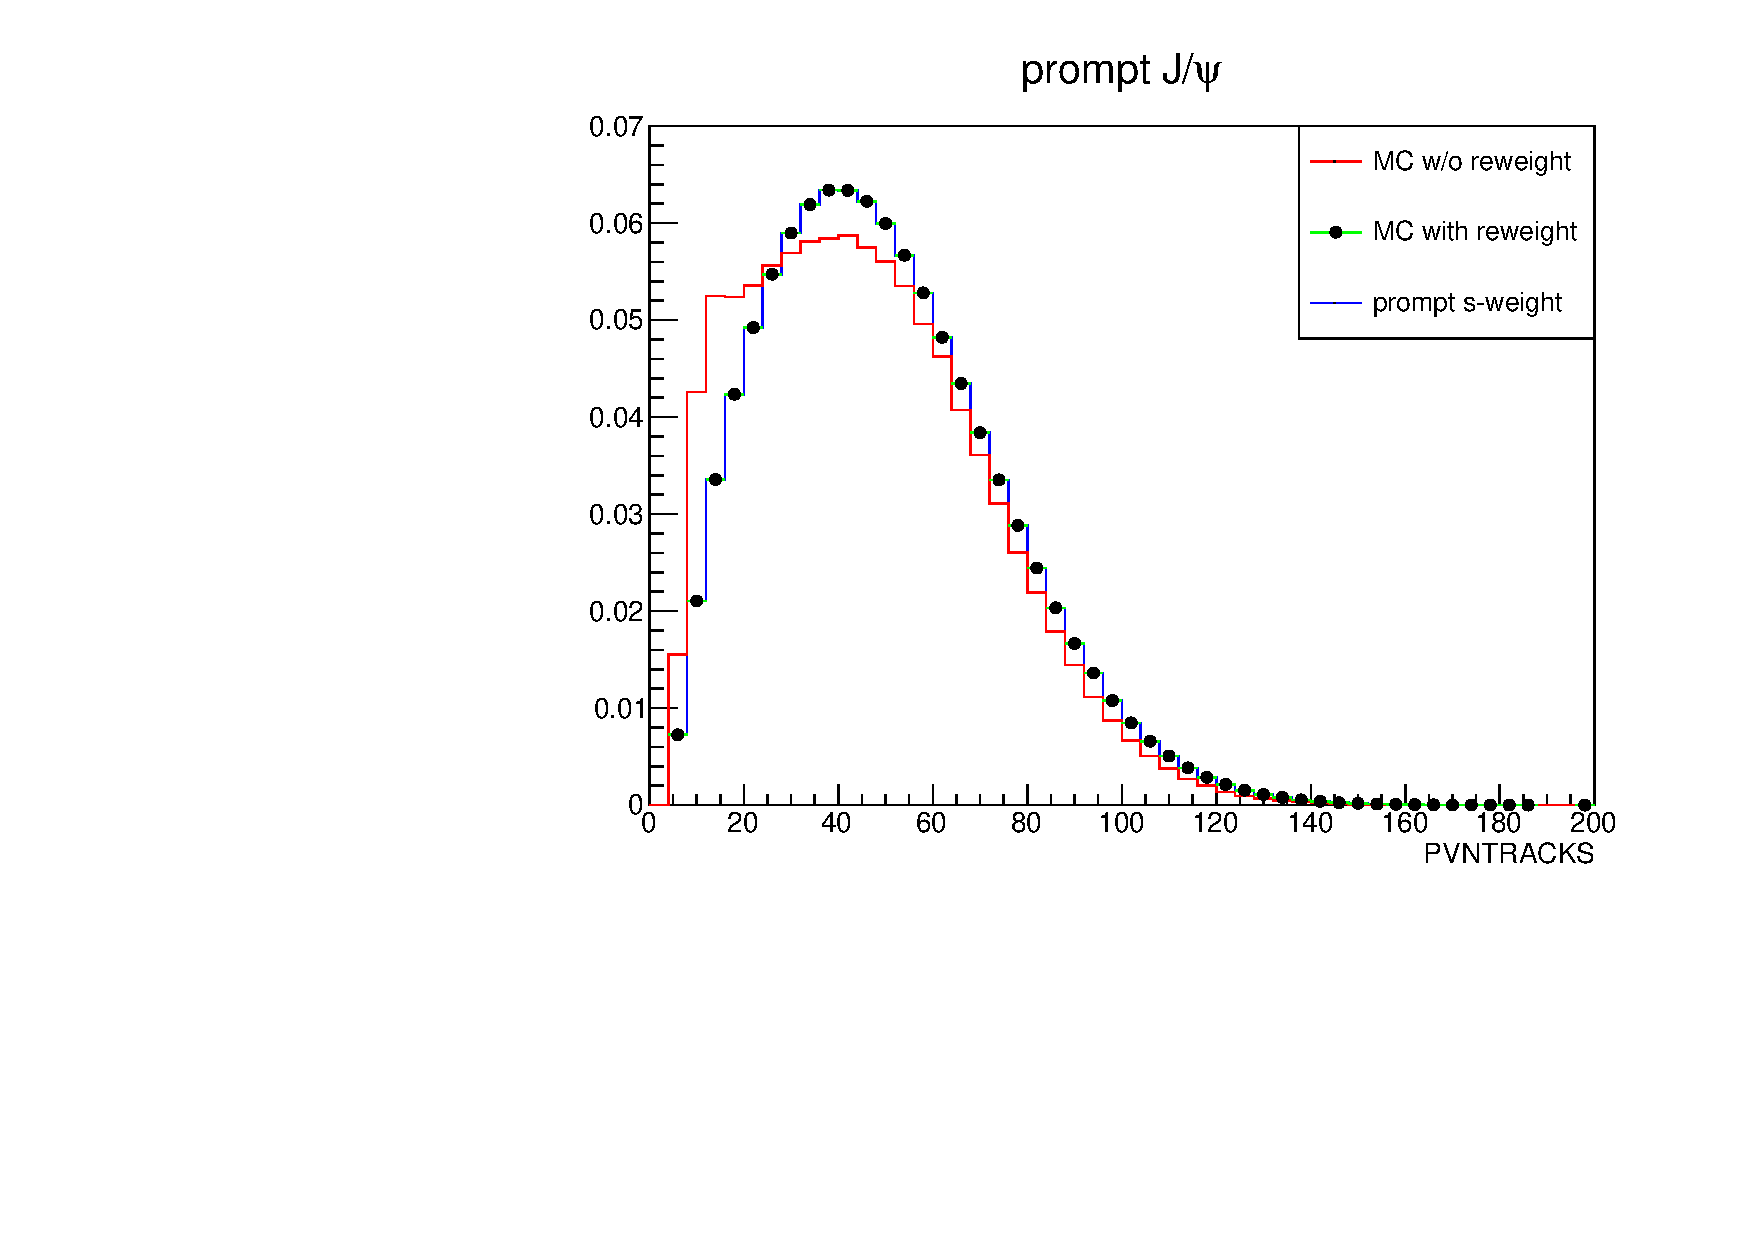
\includegraphics[width=0.25\linewidth]{pdf/Jpsi/reweight/np.pdf}
      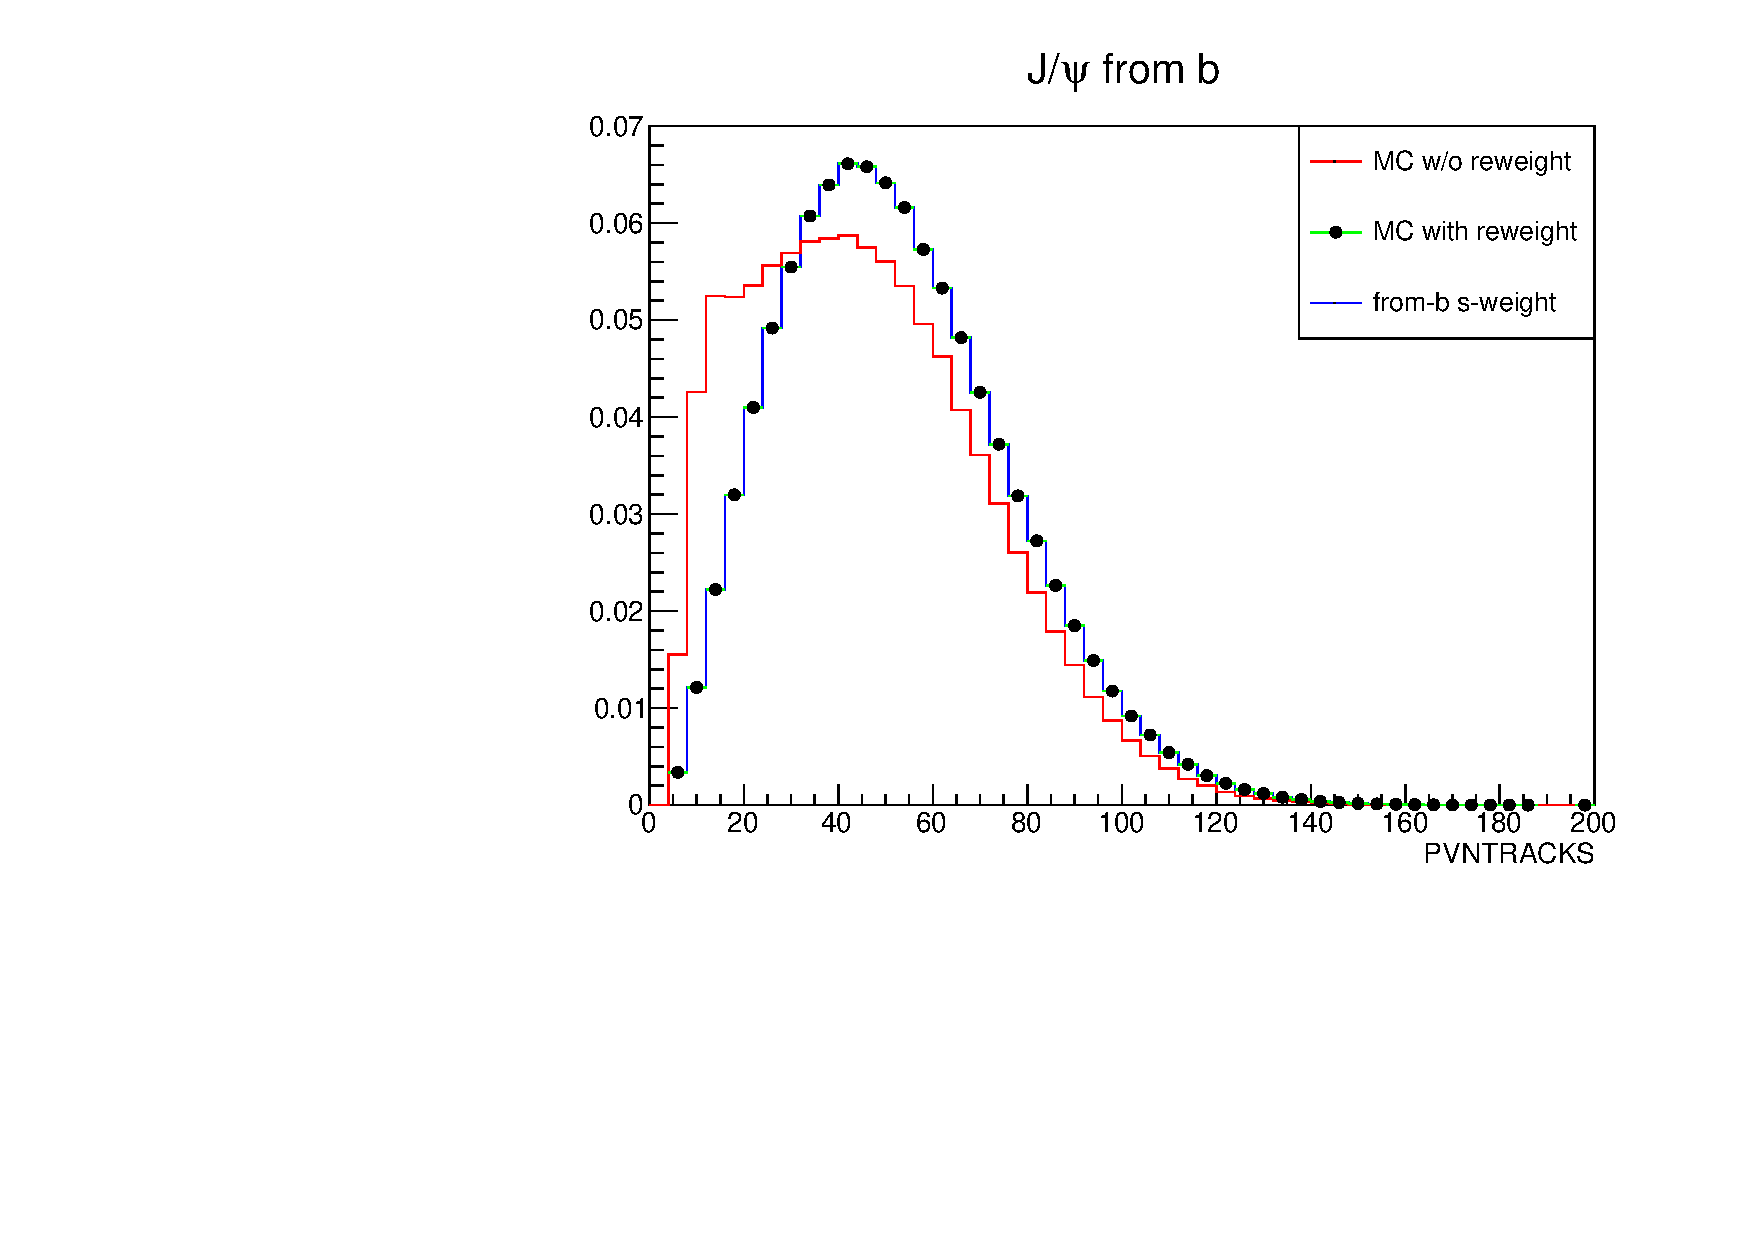
\includegraphics[width=0.25\linewidth]{pdf/Jpsi/reweight/nb.pdf}
      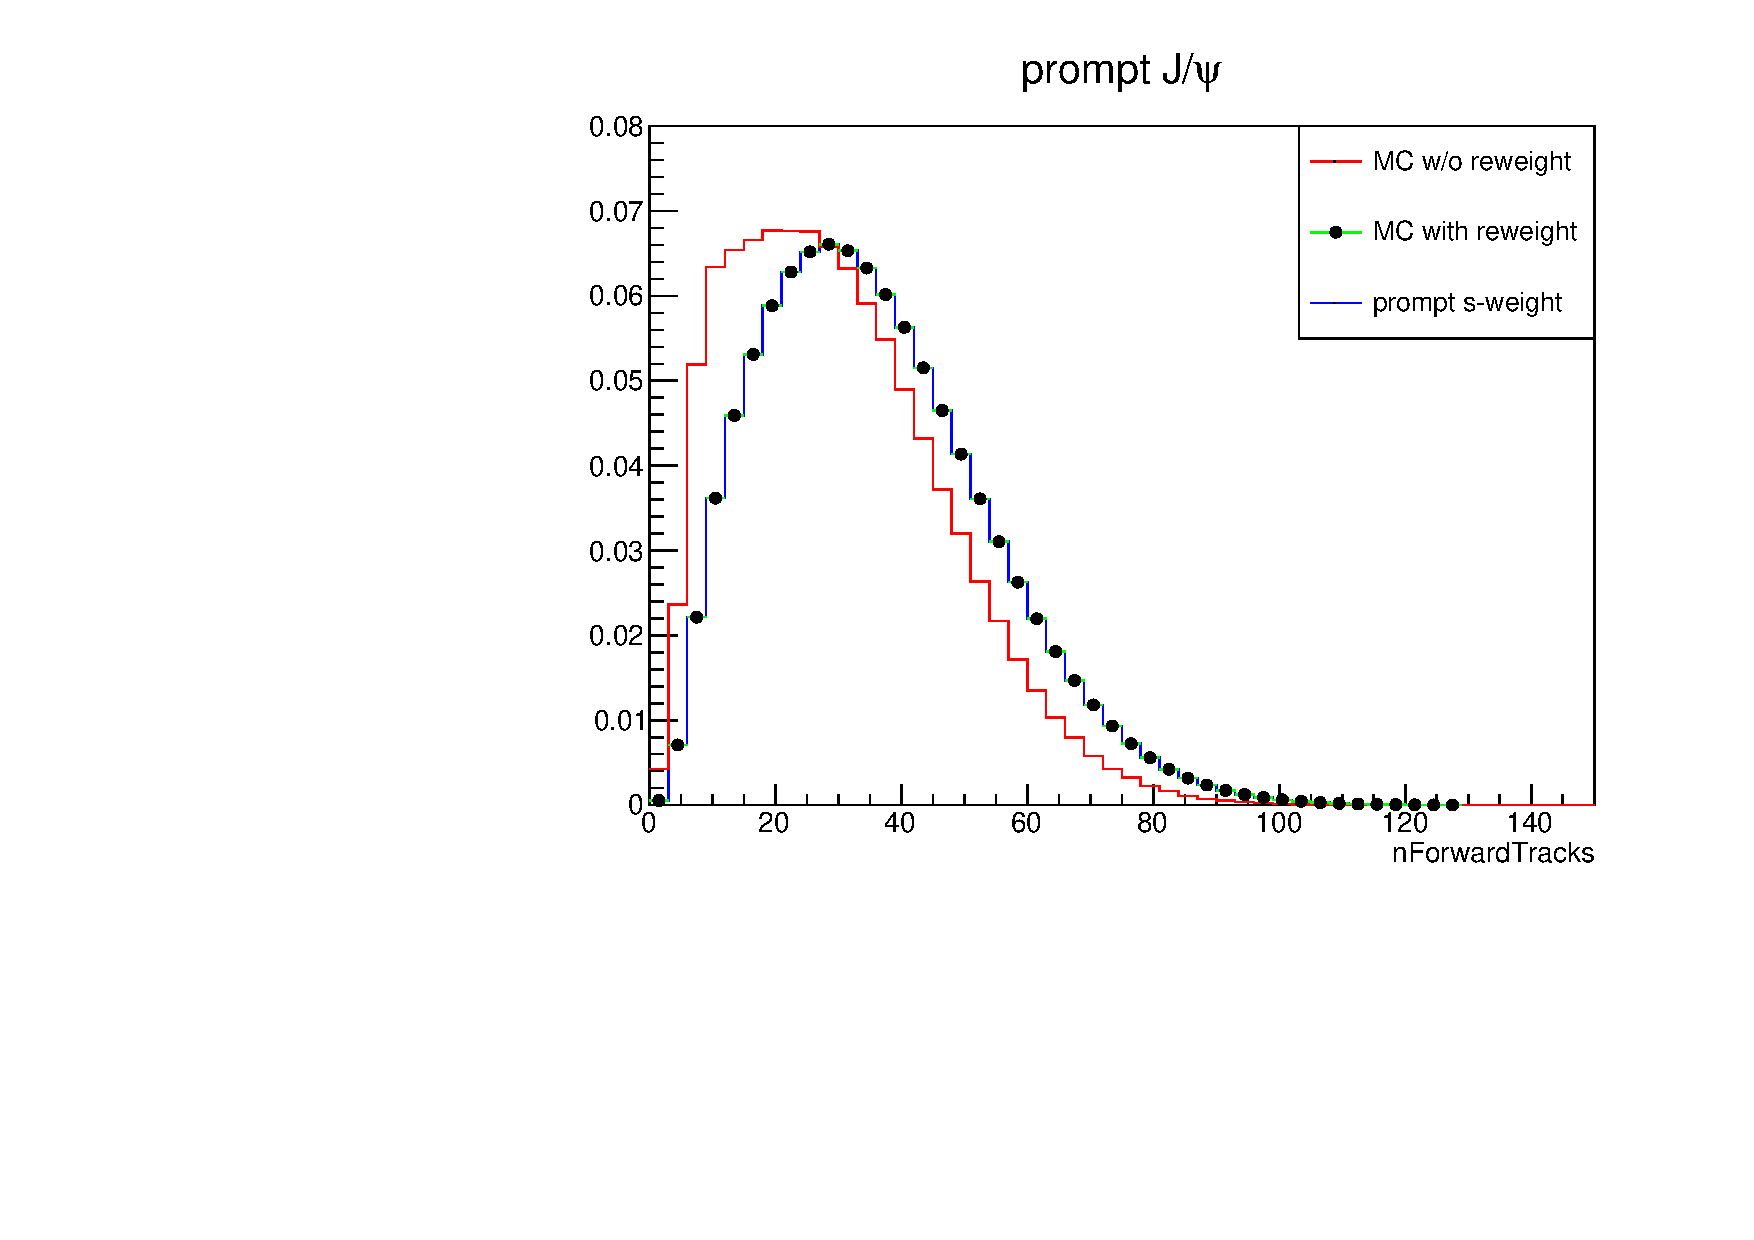
\includegraphics[width=0.25\linewidth]{pdf/Jpsi/reweight/npF.pdf}
      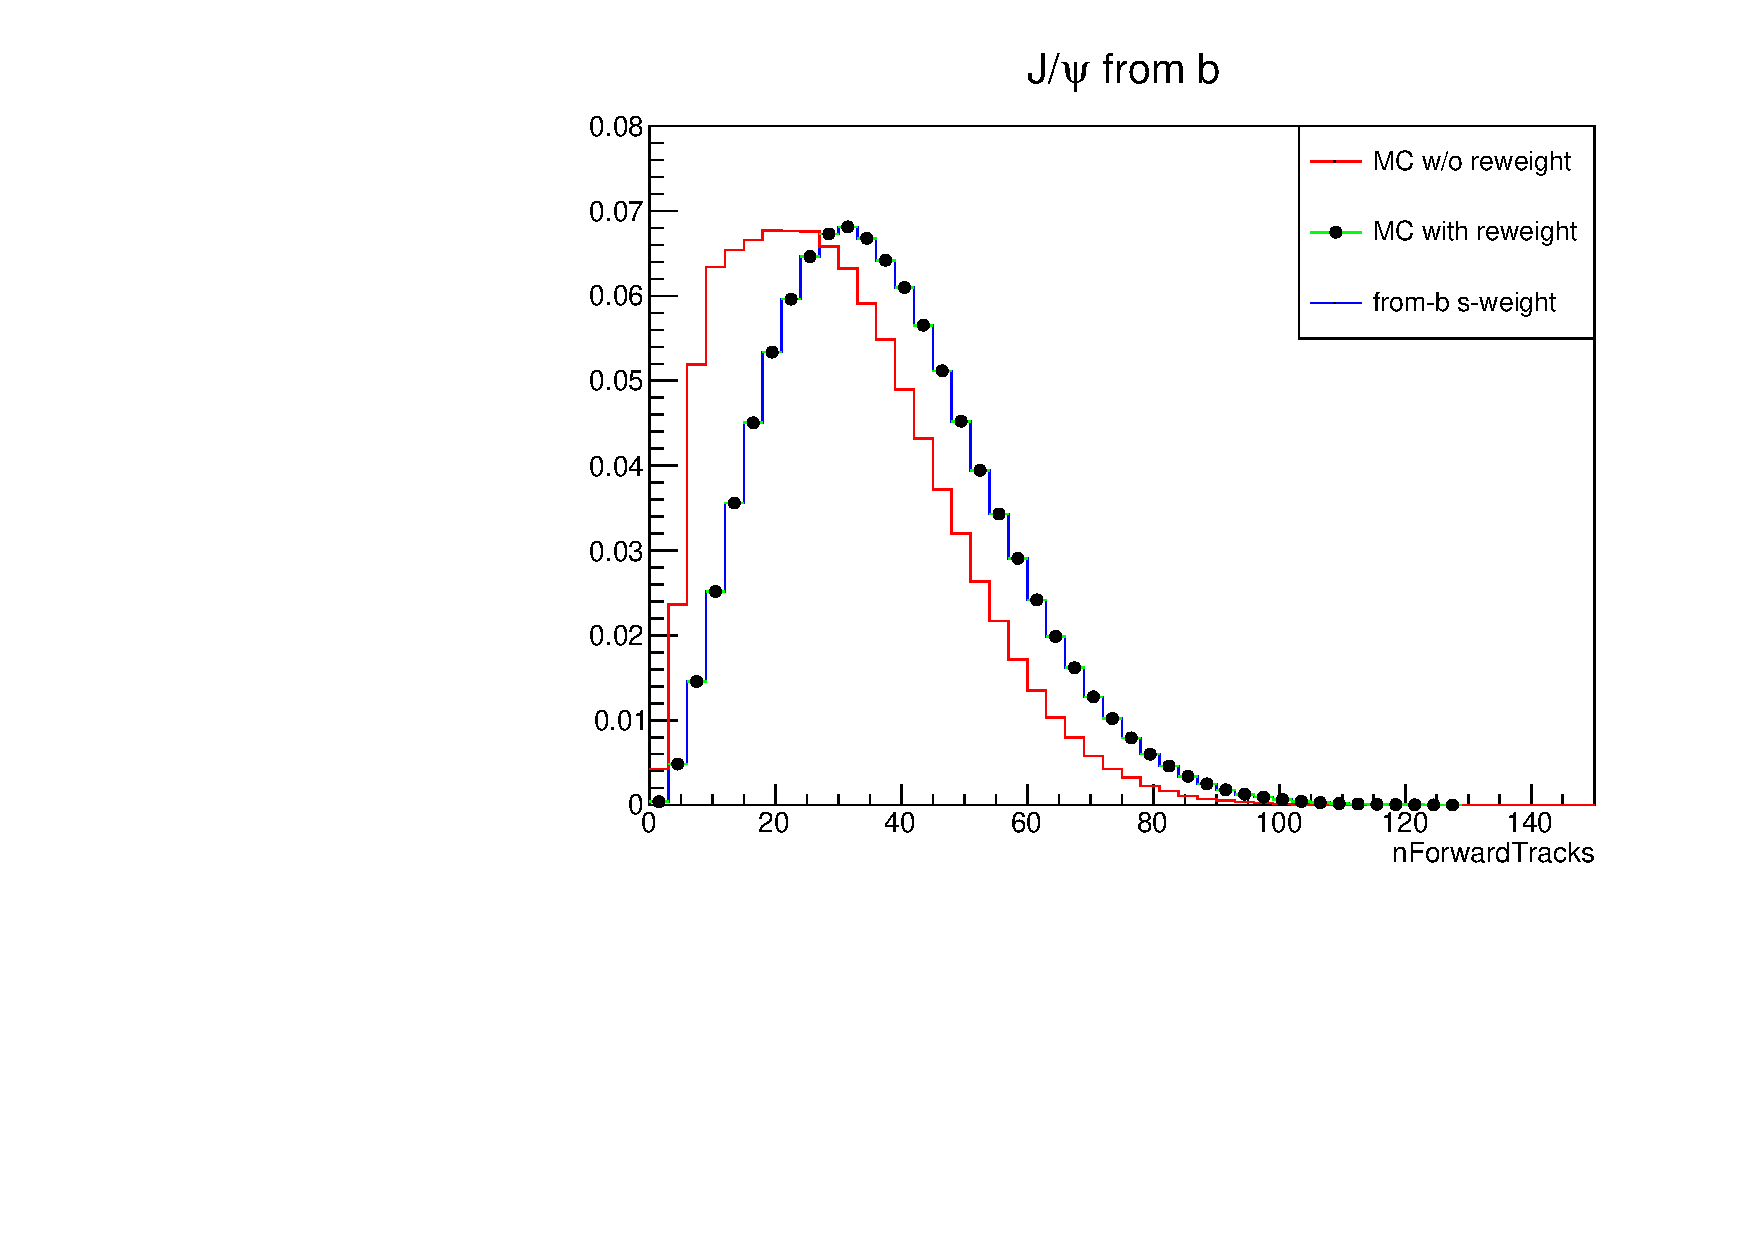
\includegraphics[width=0.25\linewidth]{pdf/Jpsi/reweight/nbF.pdf}
      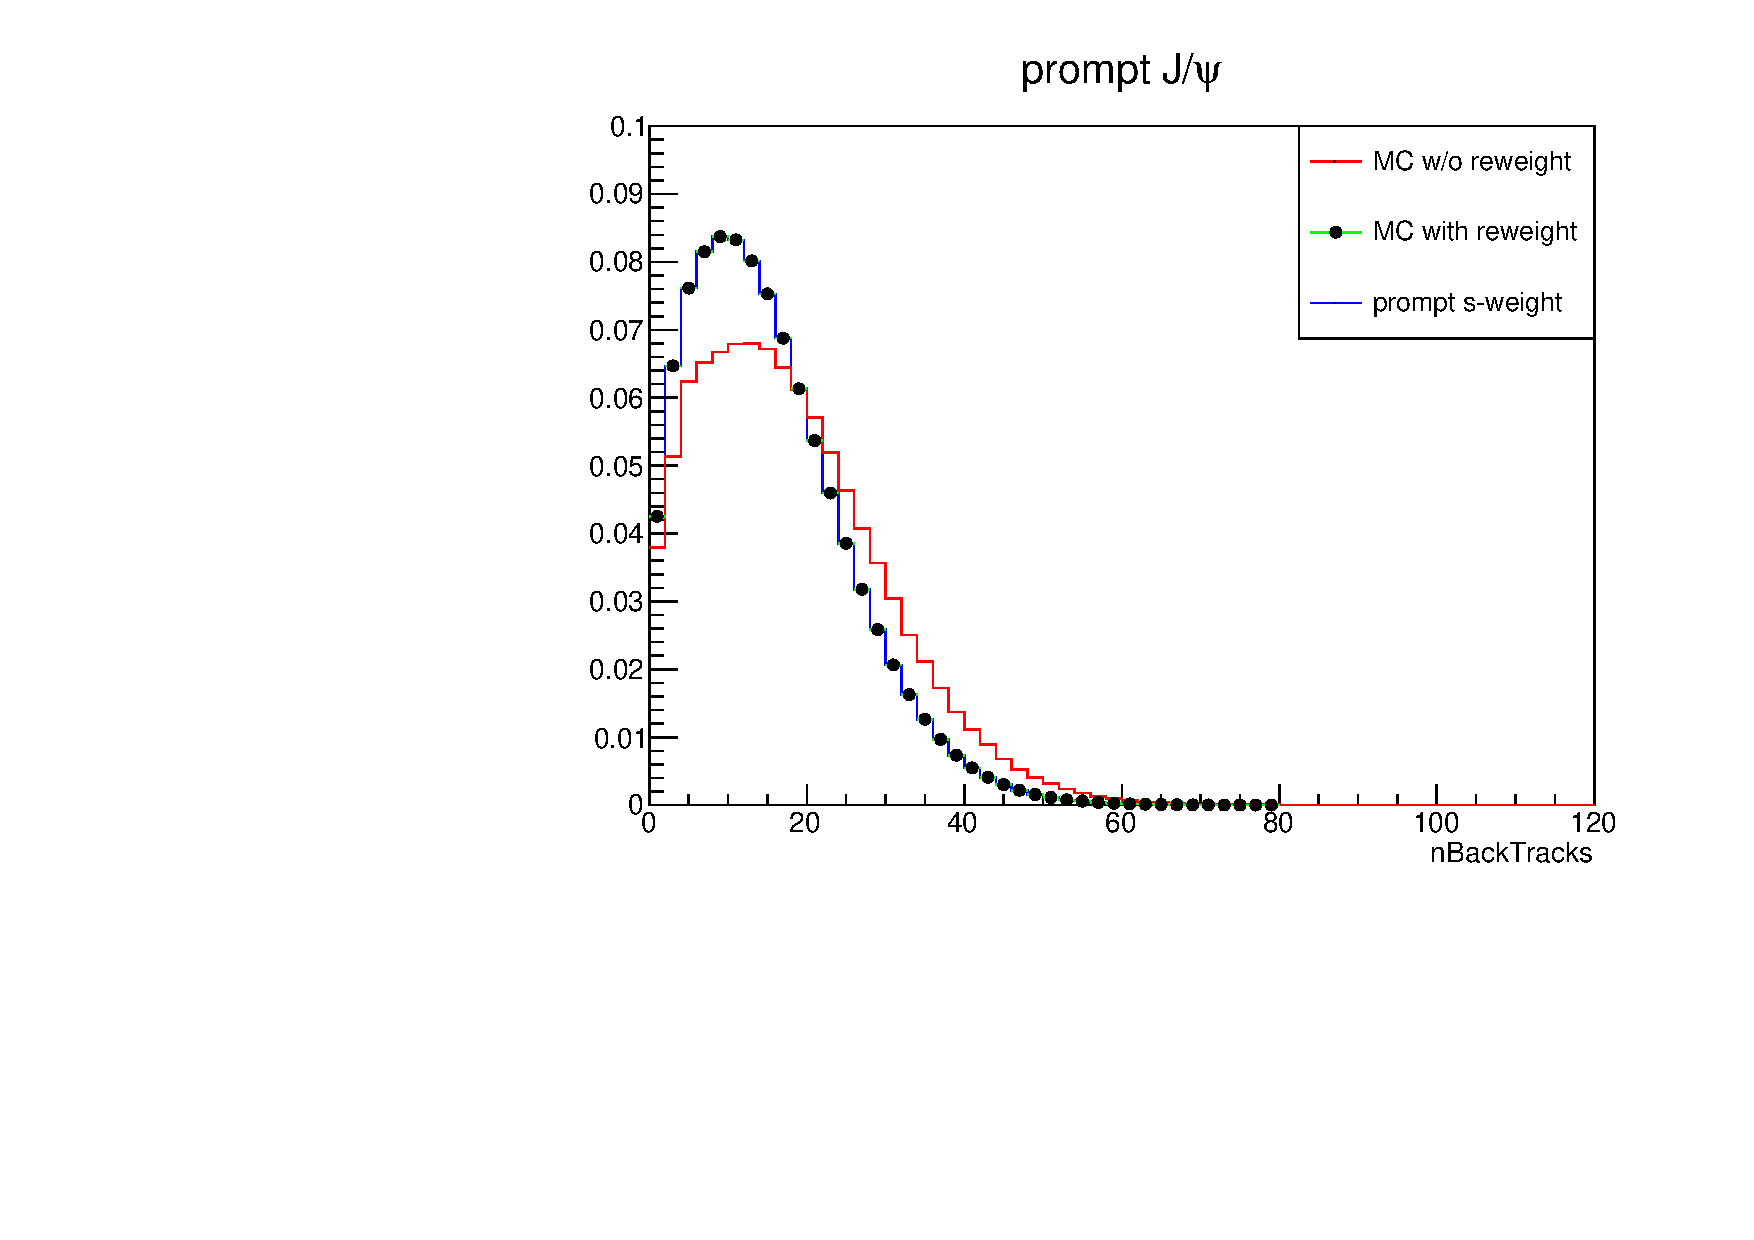
\includegraphics[width=0.25\linewidth]{pdf/Jpsi/reweight/npB.pdf}
      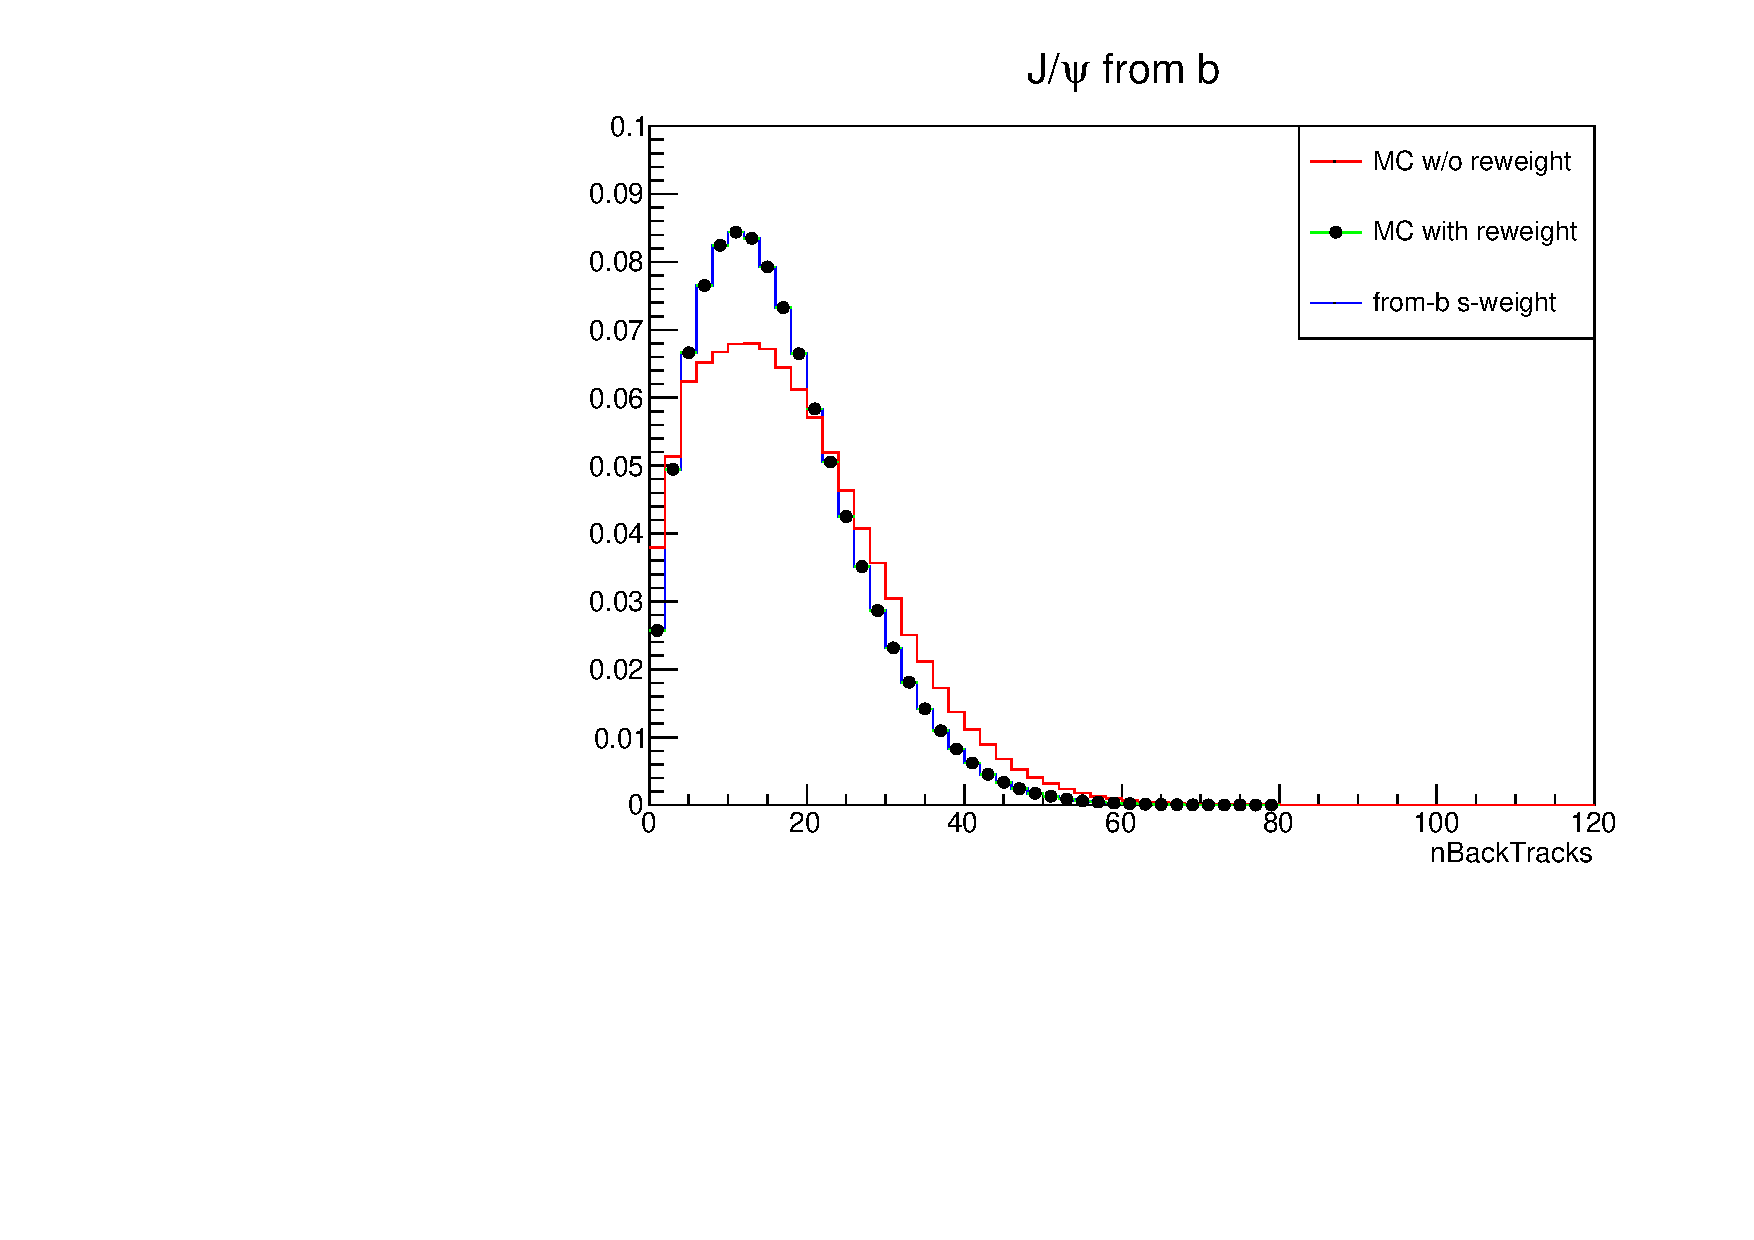
\includegraphics[width=0.25\linewidth]{pdf/Jpsi/reweight/nbB.pdf}
      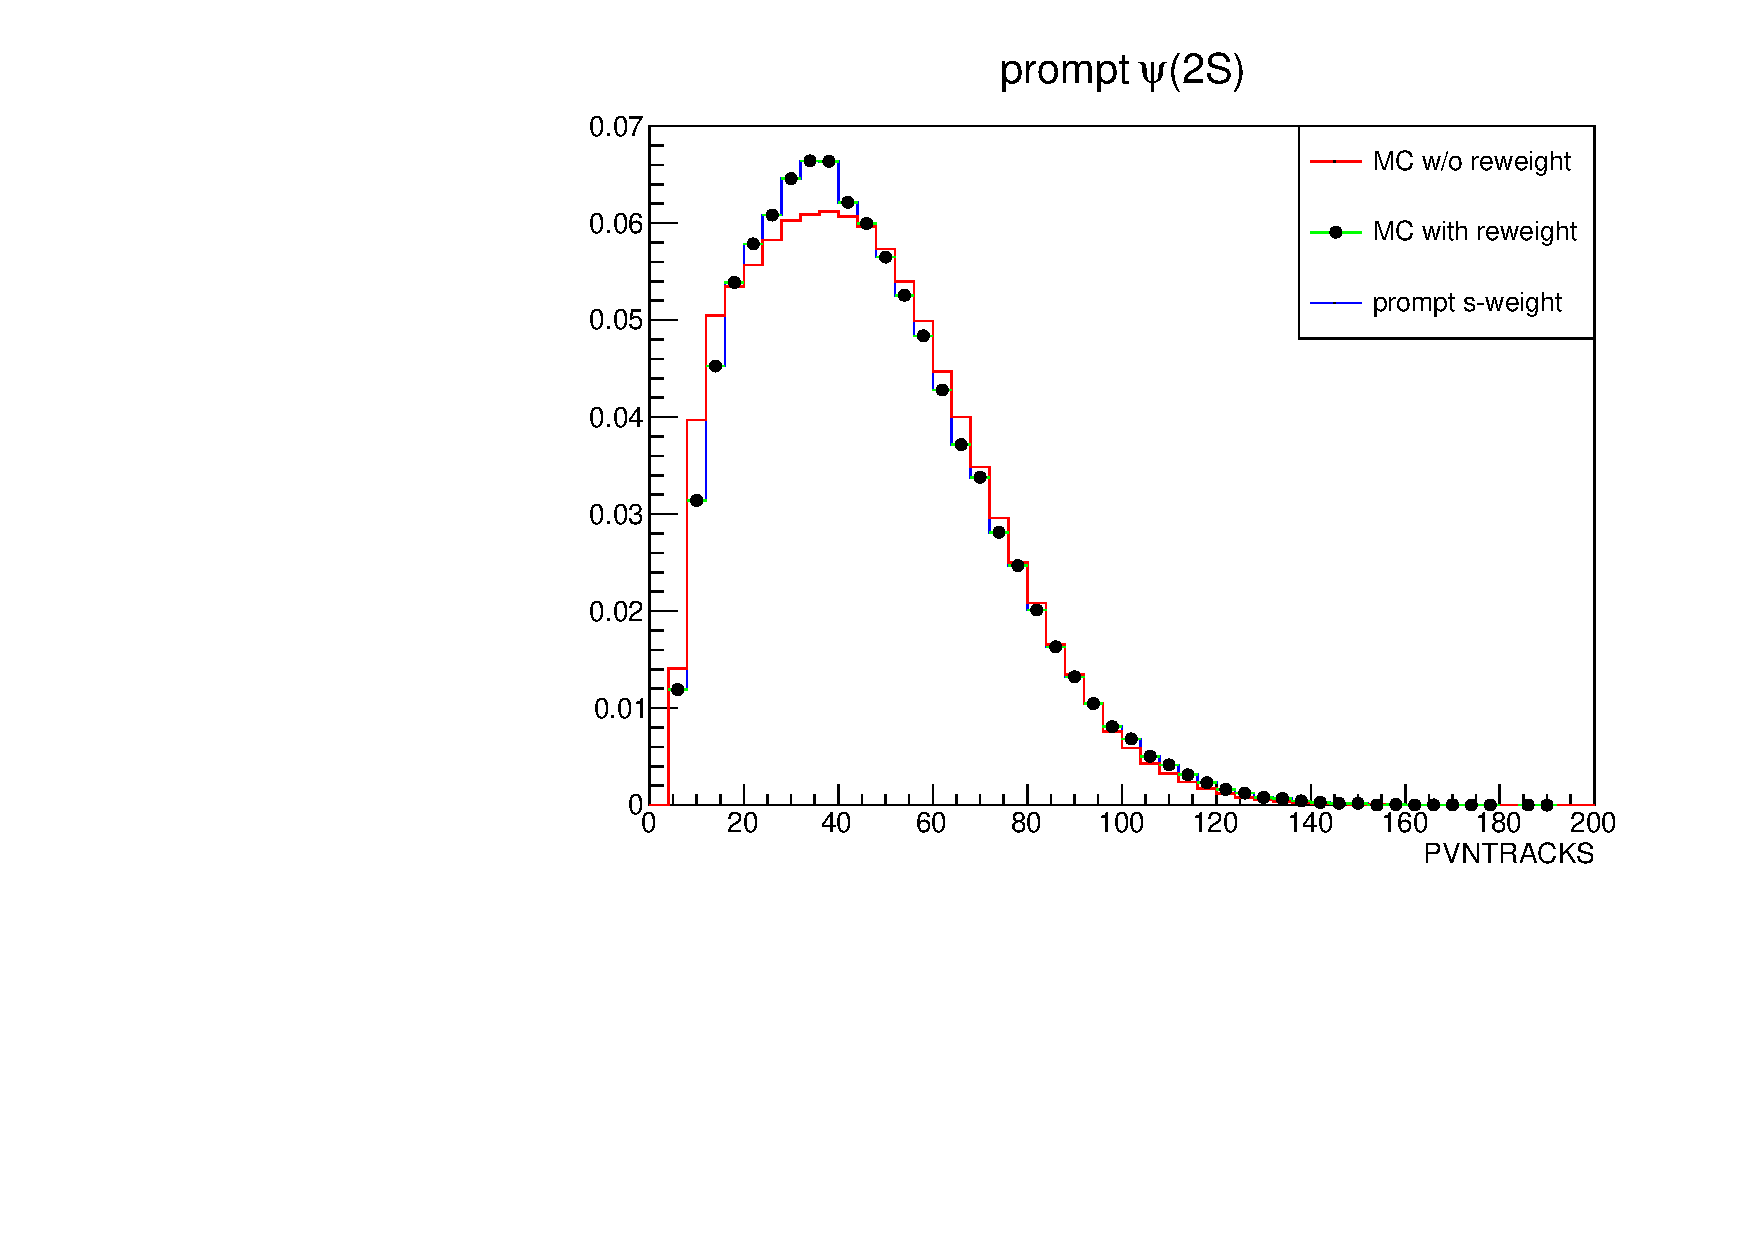
\includegraphics[width=0.25\linewidth]{pdf/Psi2S/reweight/np.pdf}
      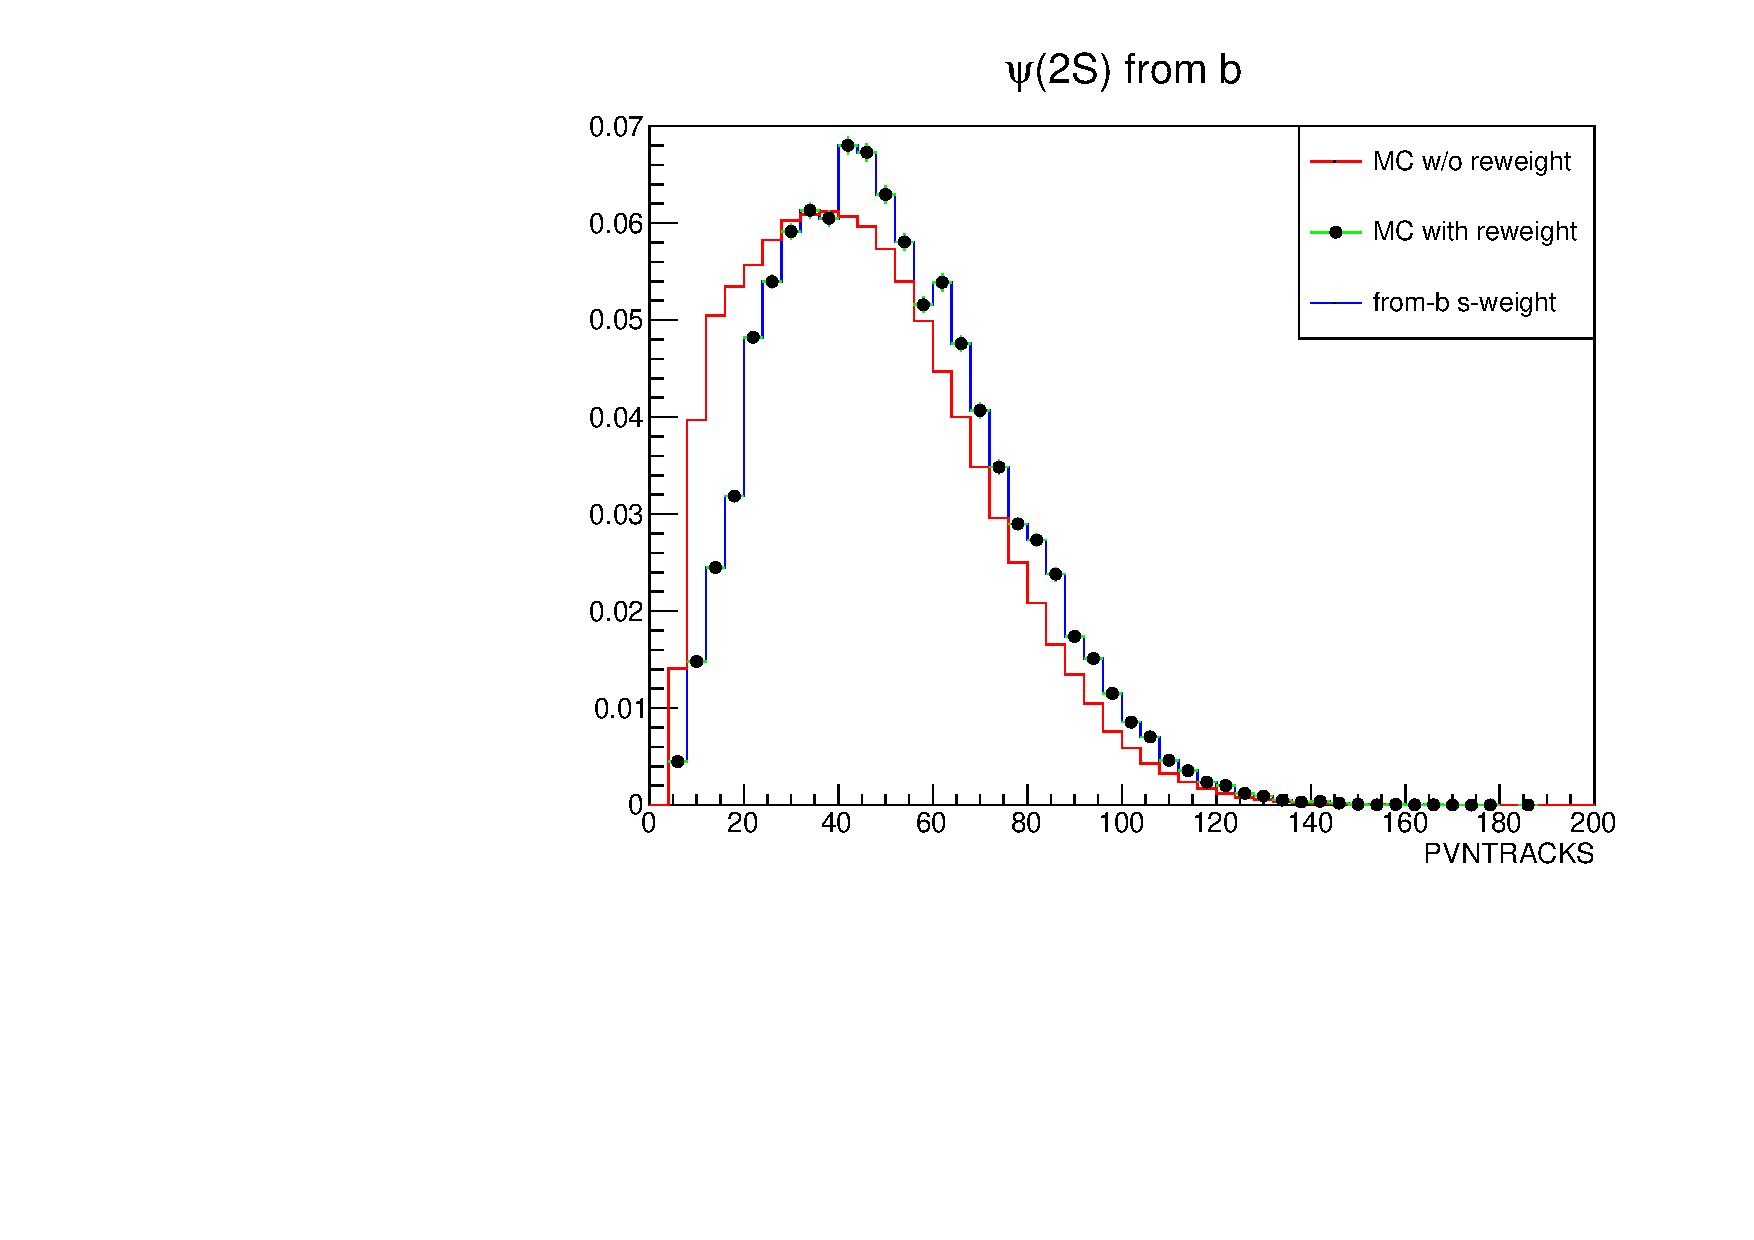
\includegraphics[width=0.25\linewidth]{pdf/Psi2S/reweight/nb.pdf}
      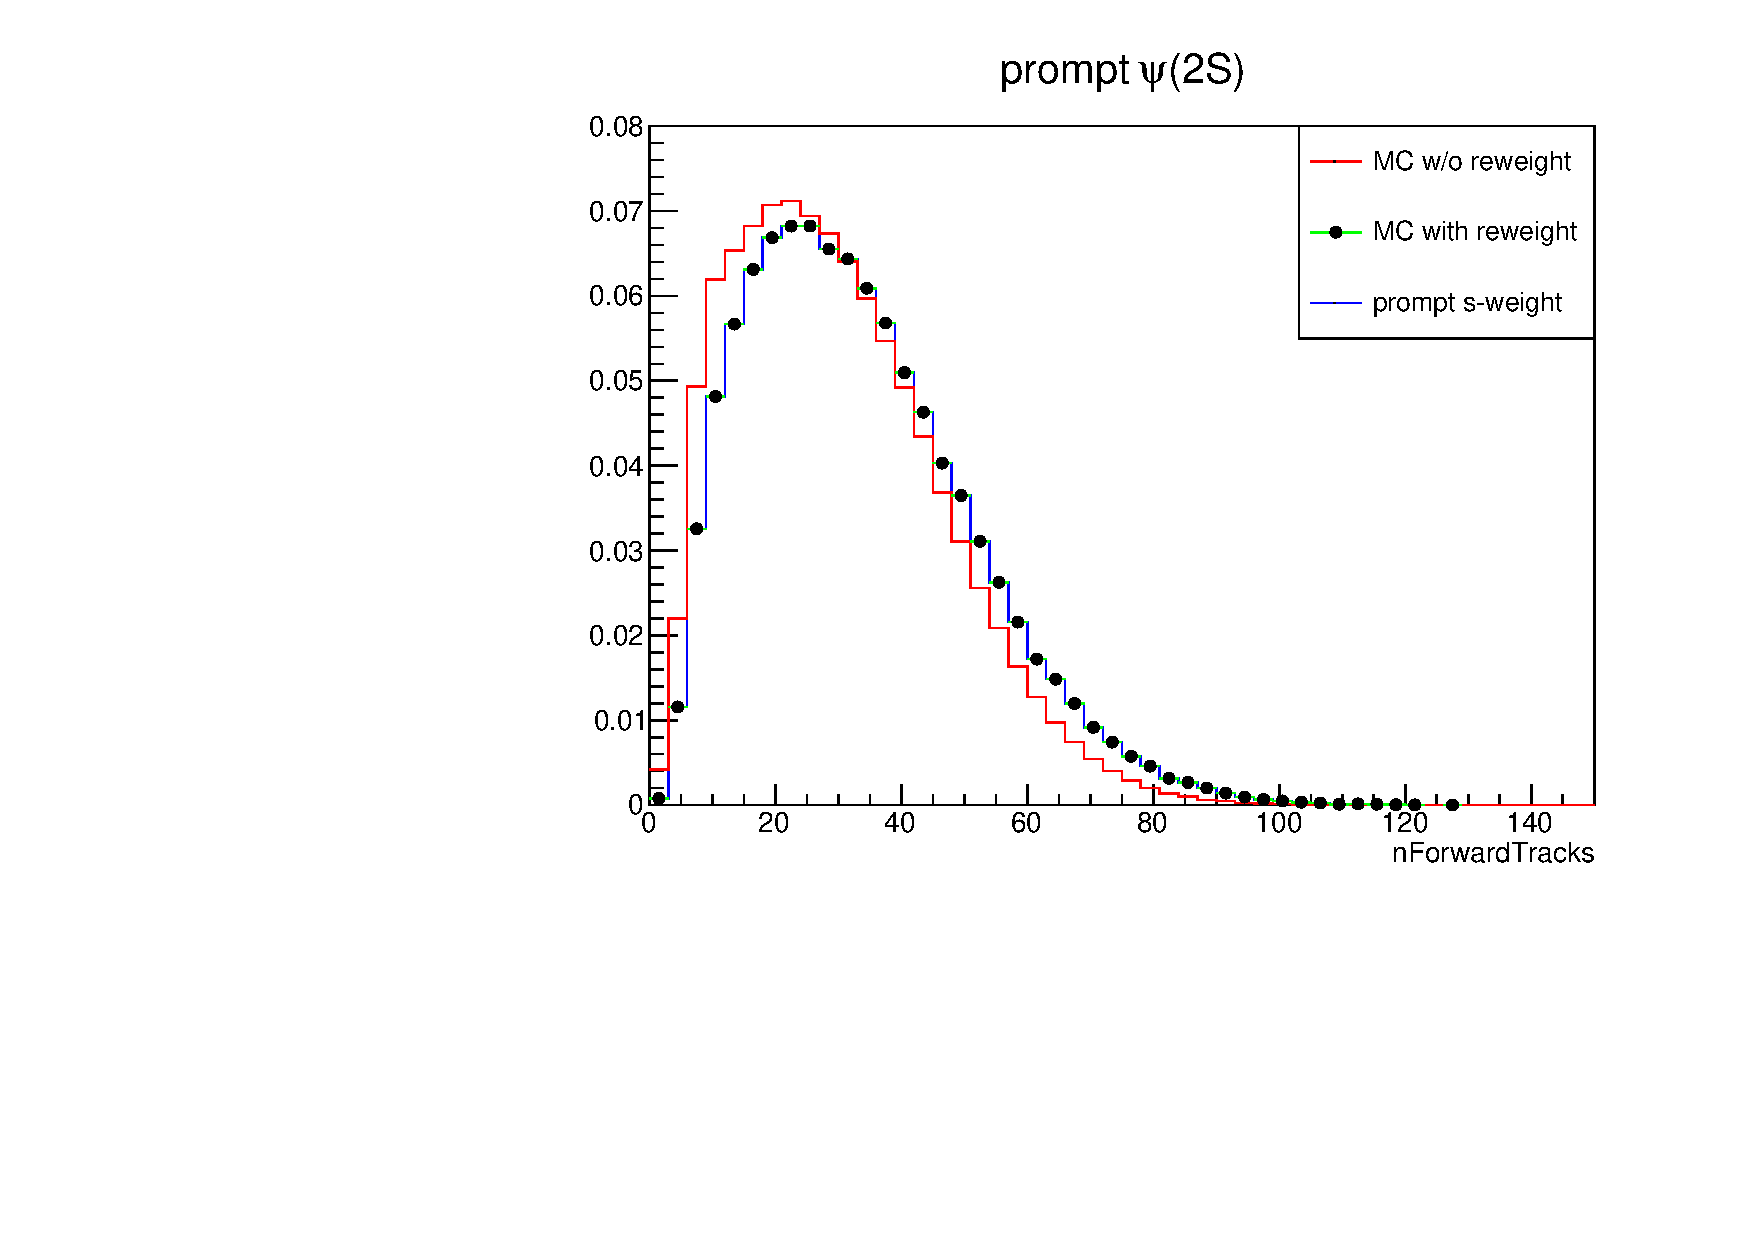
\includegraphics[width=0.25\linewidth]{pdf/Psi2S/reweight/npF.pdf}
      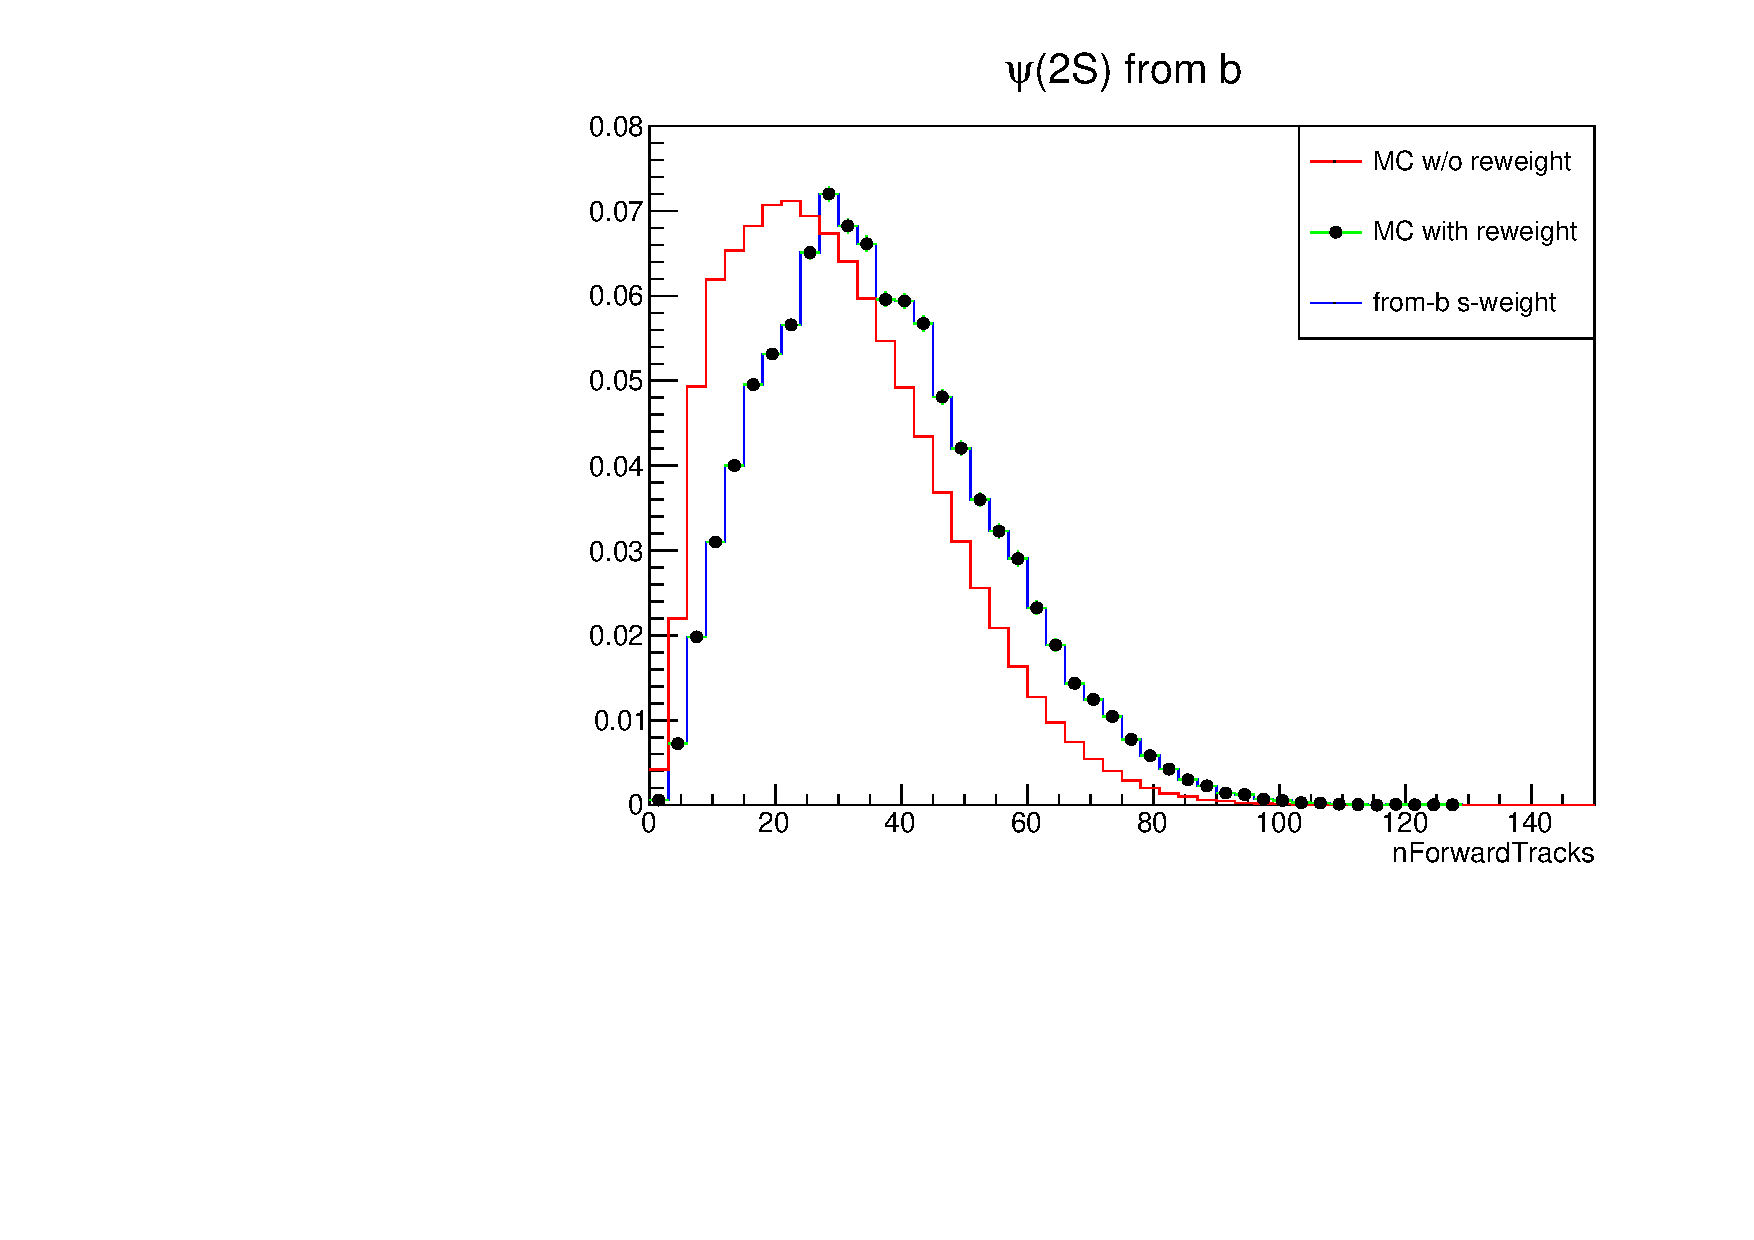
\includegraphics[width=0.25\linewidth]{pdf/Psi2S/reweight/nbF.pdf}
      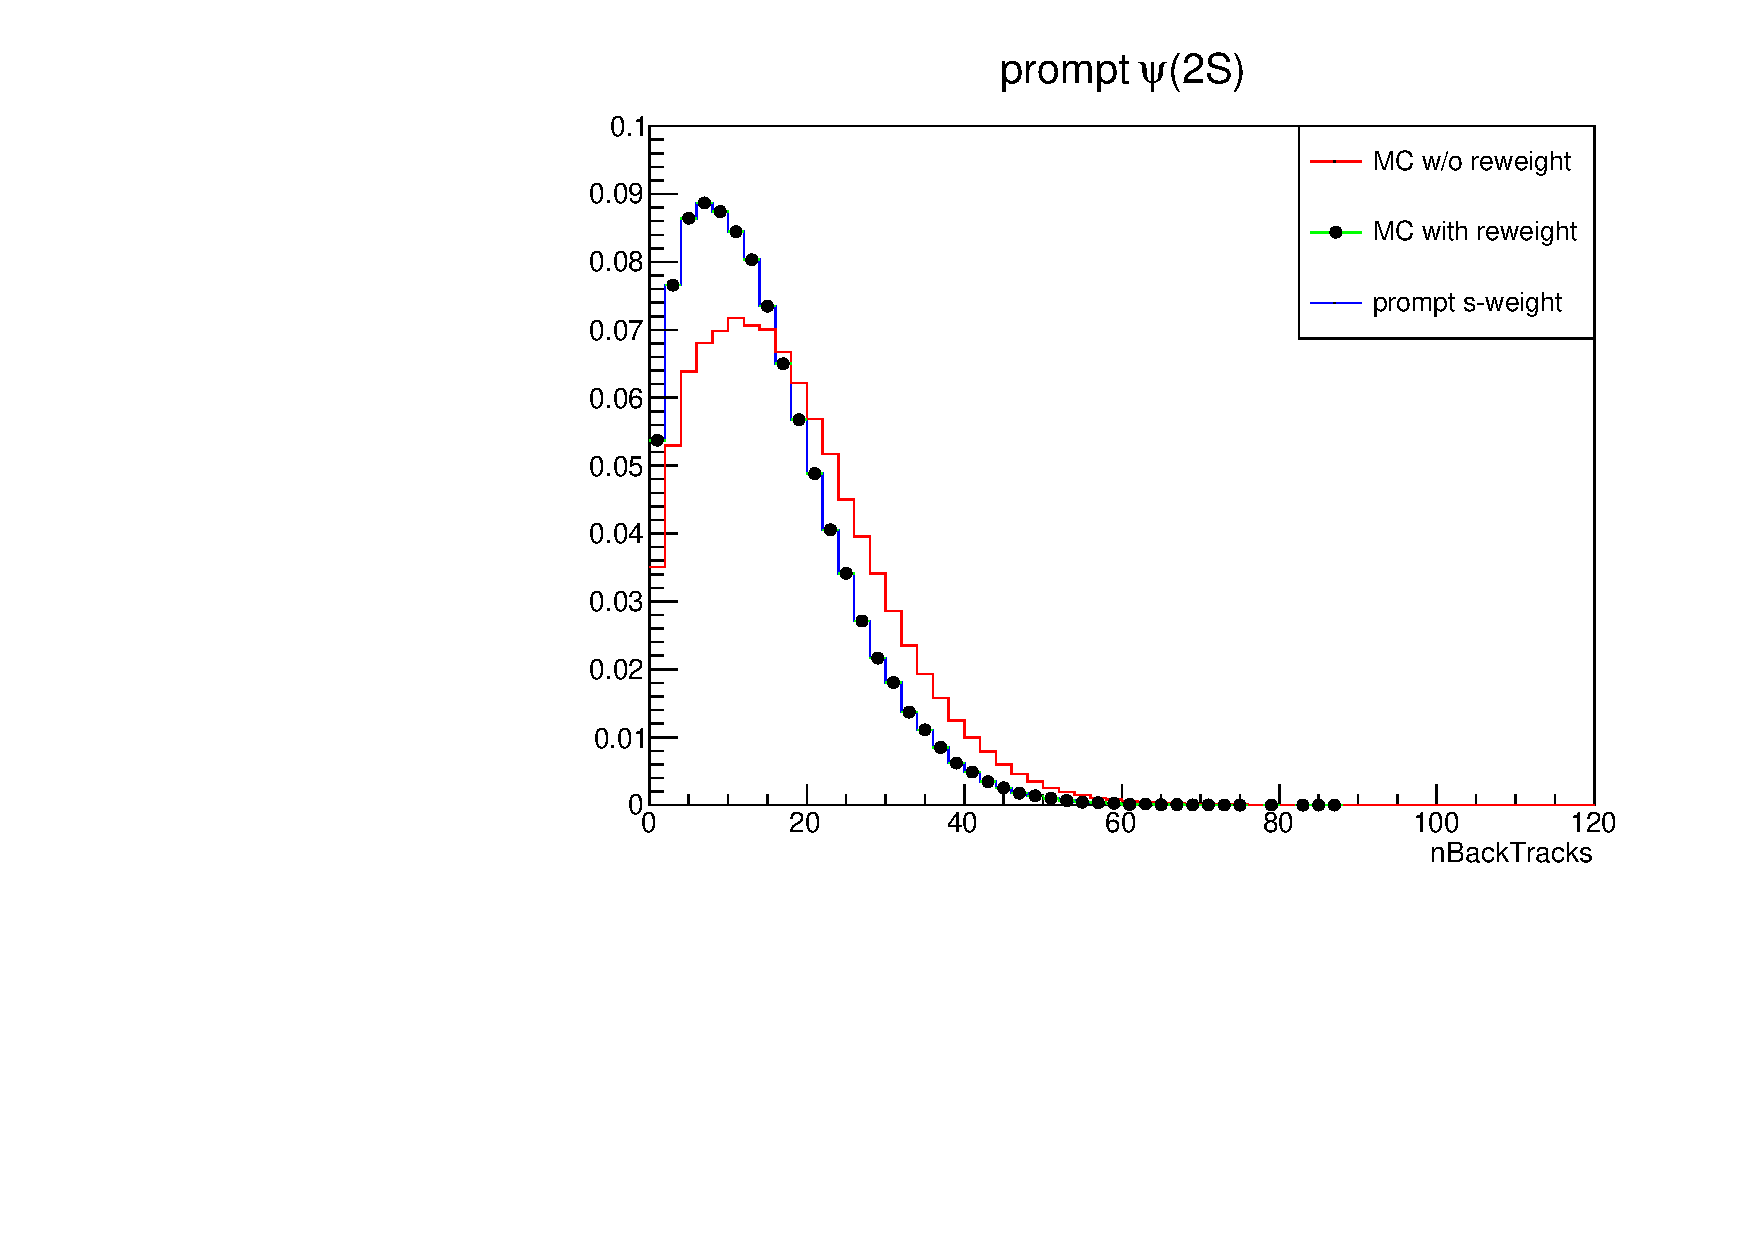
\includegraphics[width=0.25\linewidth]{pdf/Psi2S/reweight/npB.pdf}
      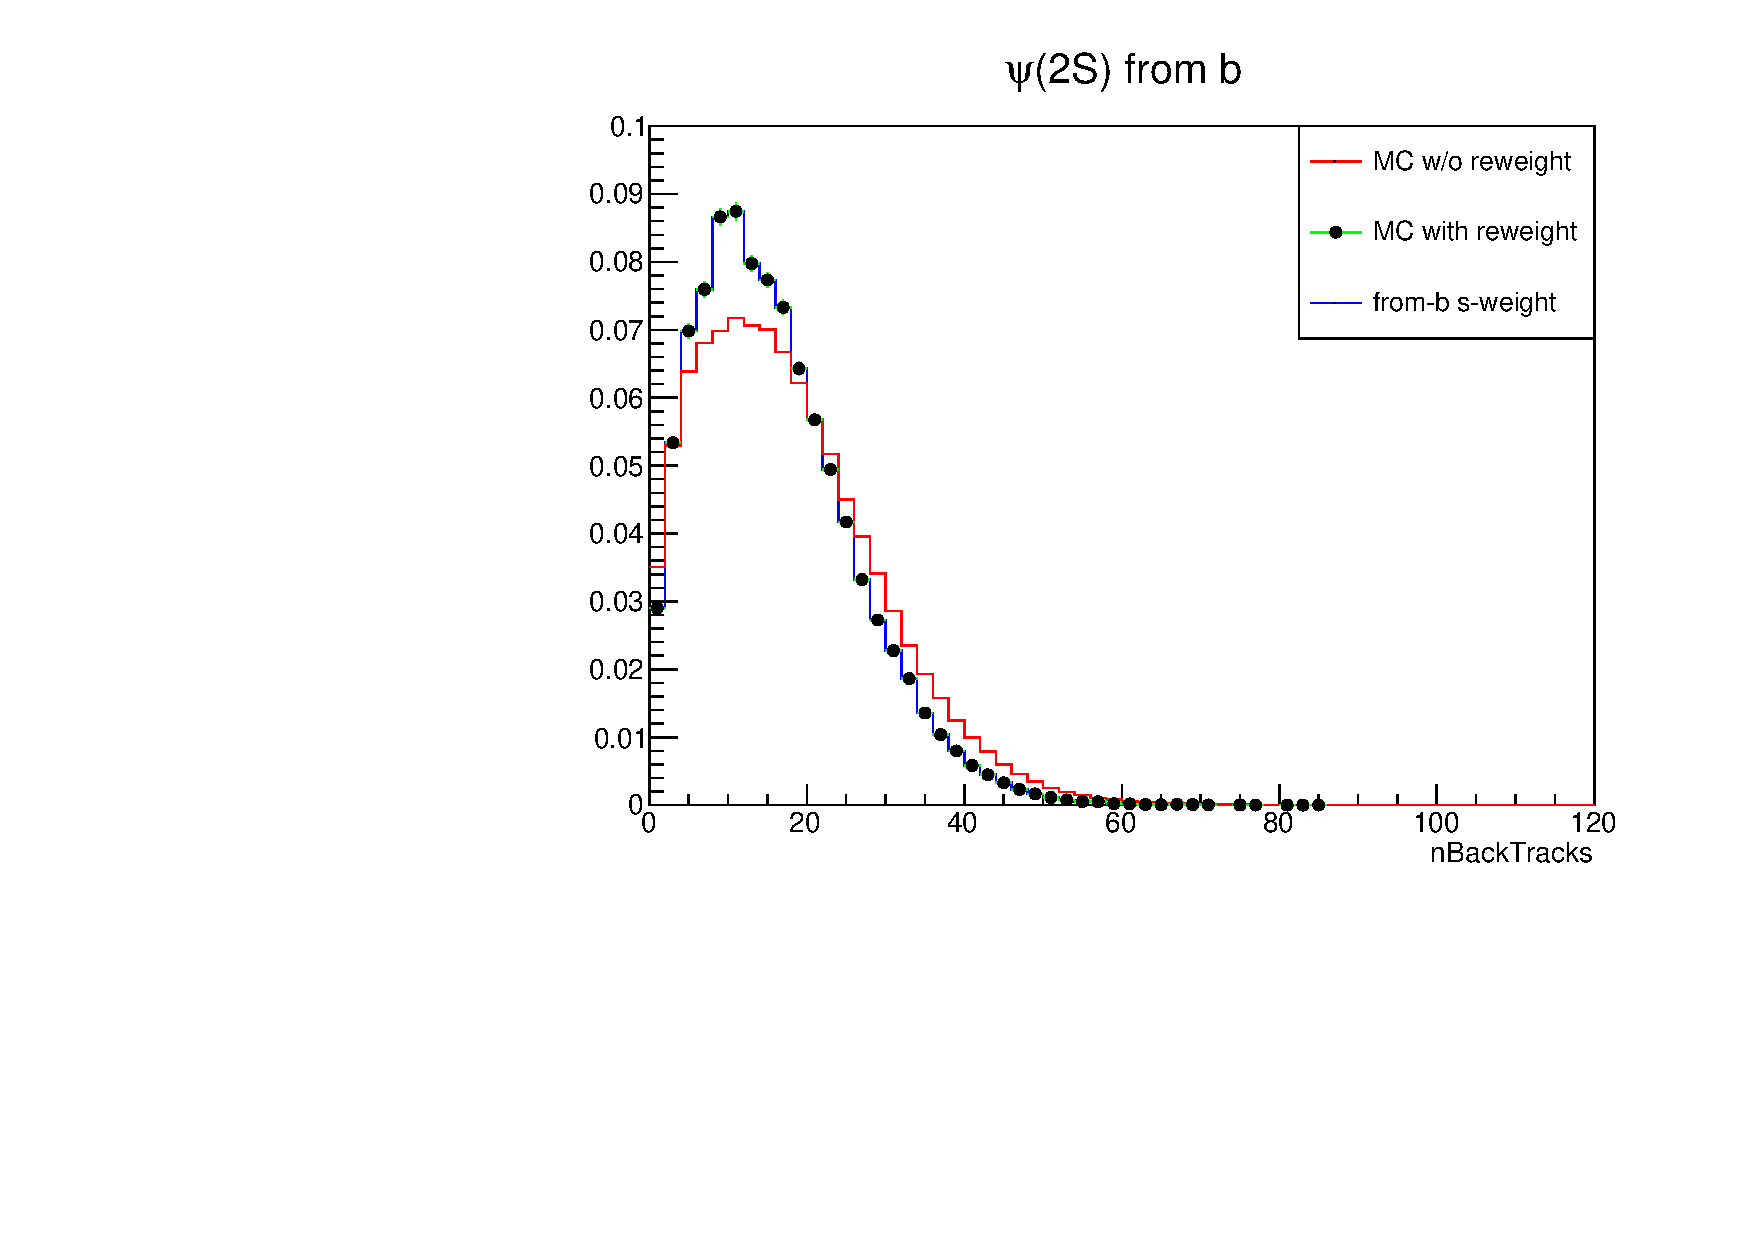
\includegraphics[width=0.25\linewidth]{pdf/Psi2S/reweight/nbB.pdf}
    \end{center}
    \caption{
      Reweight the multiplicity distribution to match MC to s-weighted data, the first two rows are reweight of \jpsi and the rest two rows are of $\psitwos$.}
    \label{reweight}
\end{figure}
For \jpsi \pt-$y$ reweight, the results cut in each $y$ region for $\jpsi$ is shown in Figs~\ref{JreweightPTY}. And the result for \psitwos is shown in Figs~\ref{PreweightPTY}.
\begin{figure}[h]
    \begin{center}
      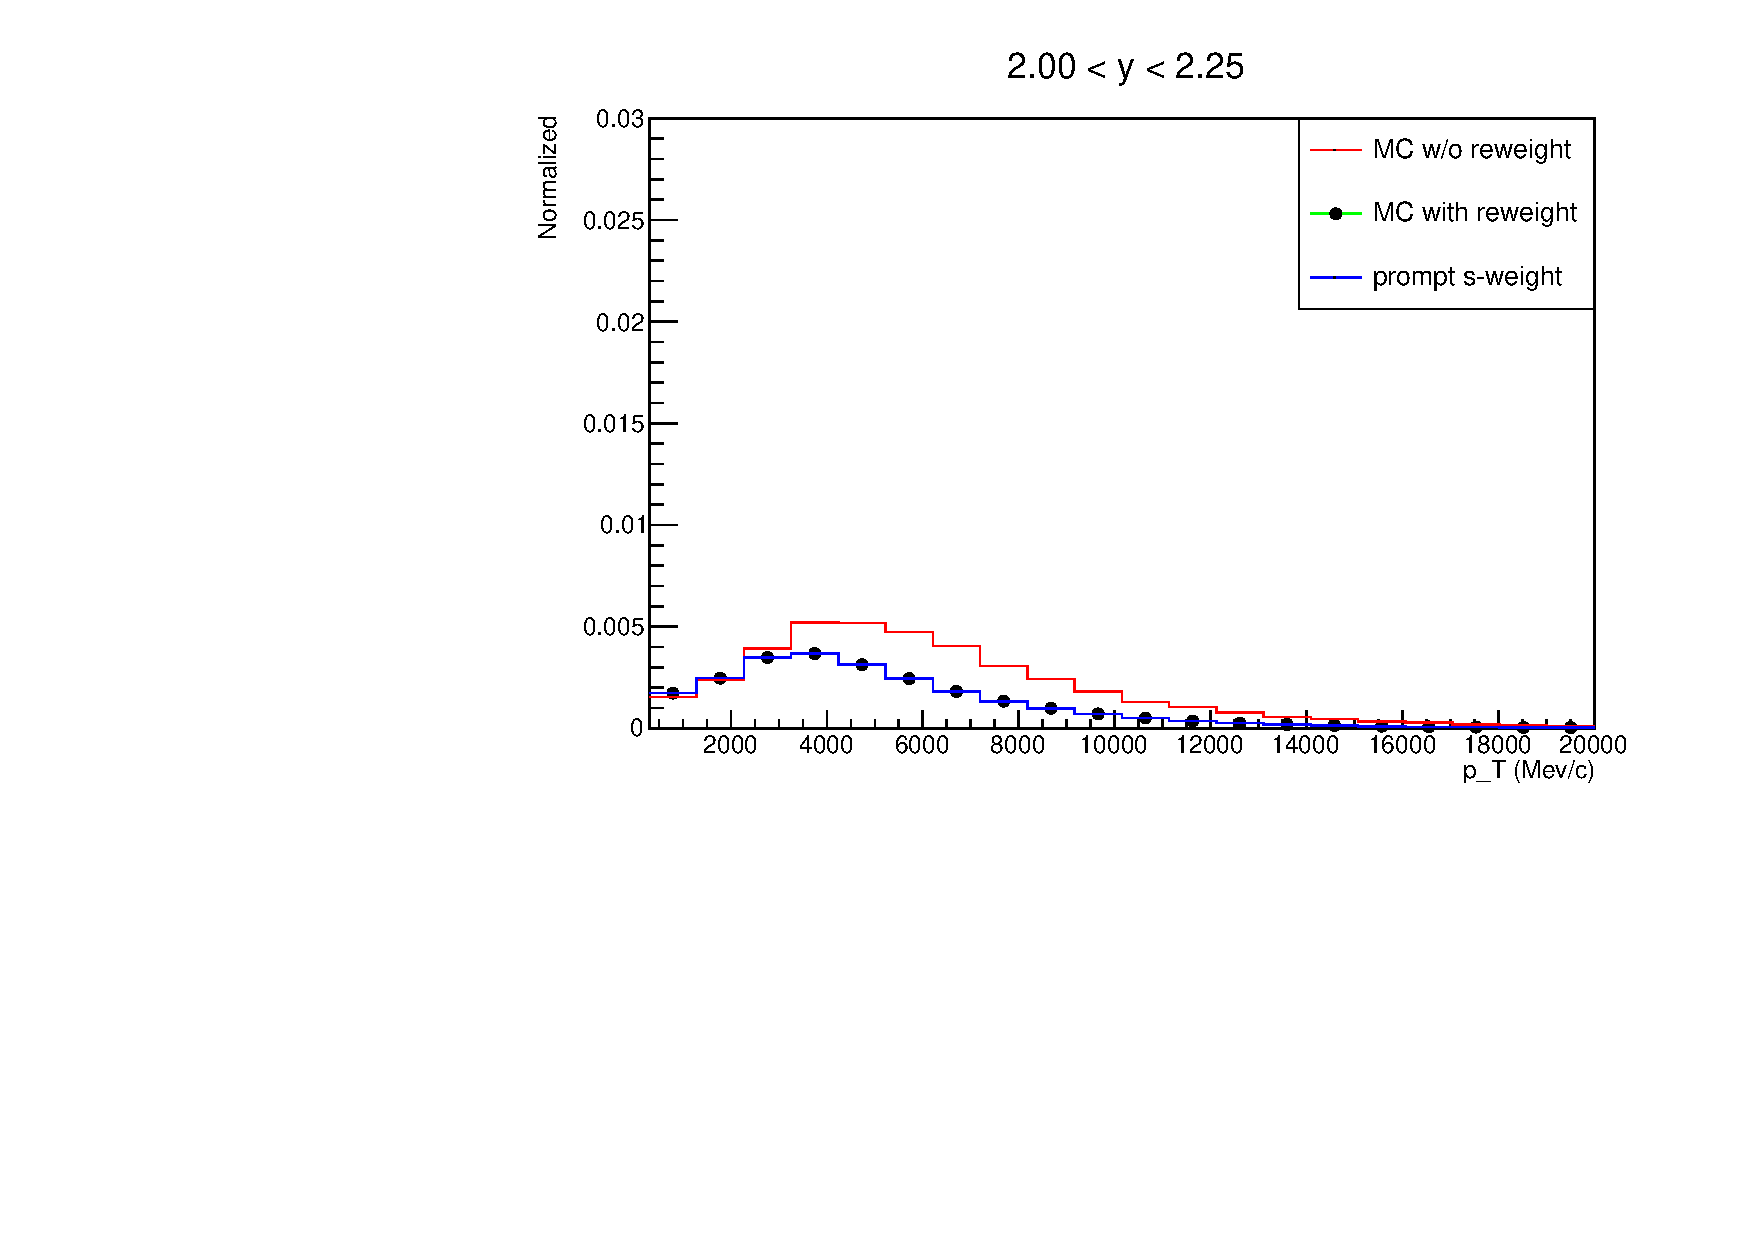
\includegraphics[width=0.19\linewidth]{pdf/Jpsi/reweight/Yp1.pdf}
      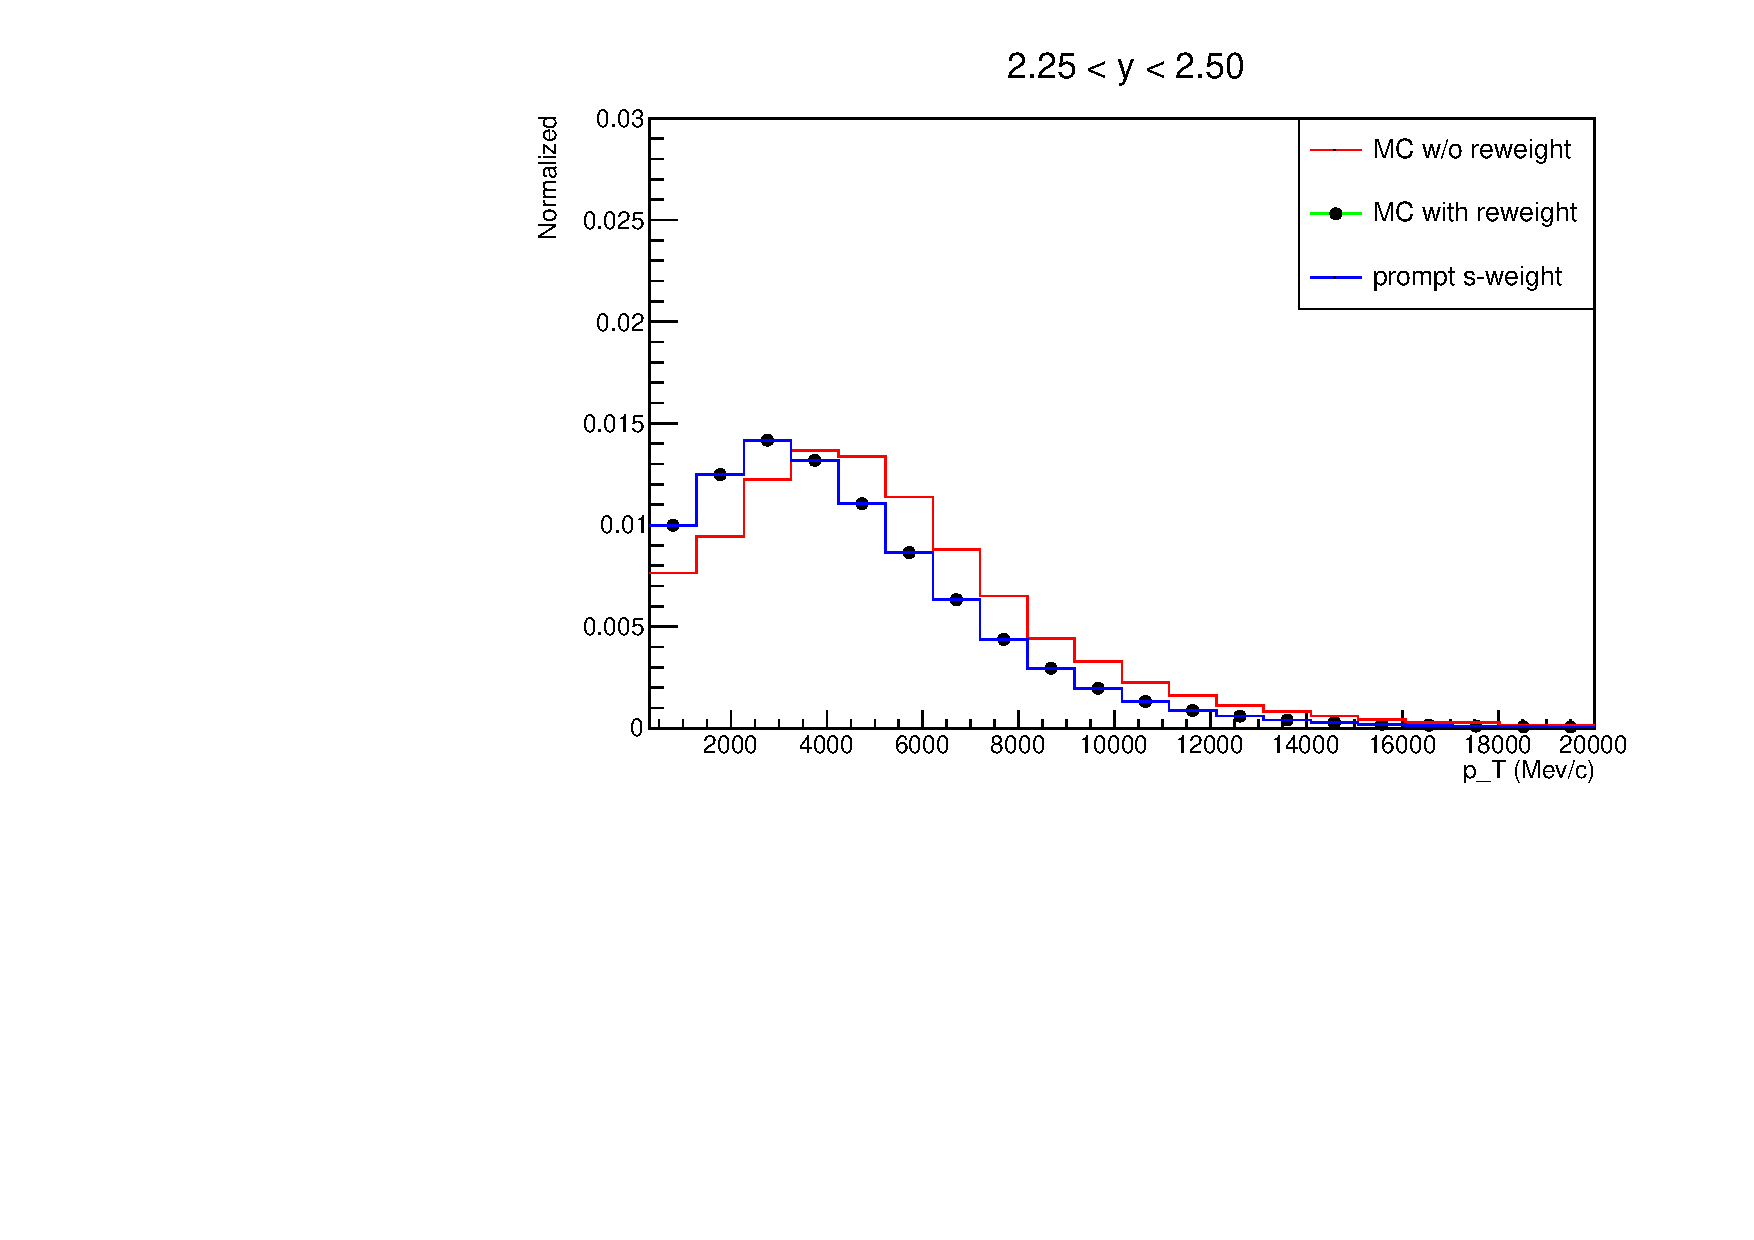
\includegraphics[width=0.19\linewidth]{pdf/Jpsi/reweight/Yp2.pdf} 
      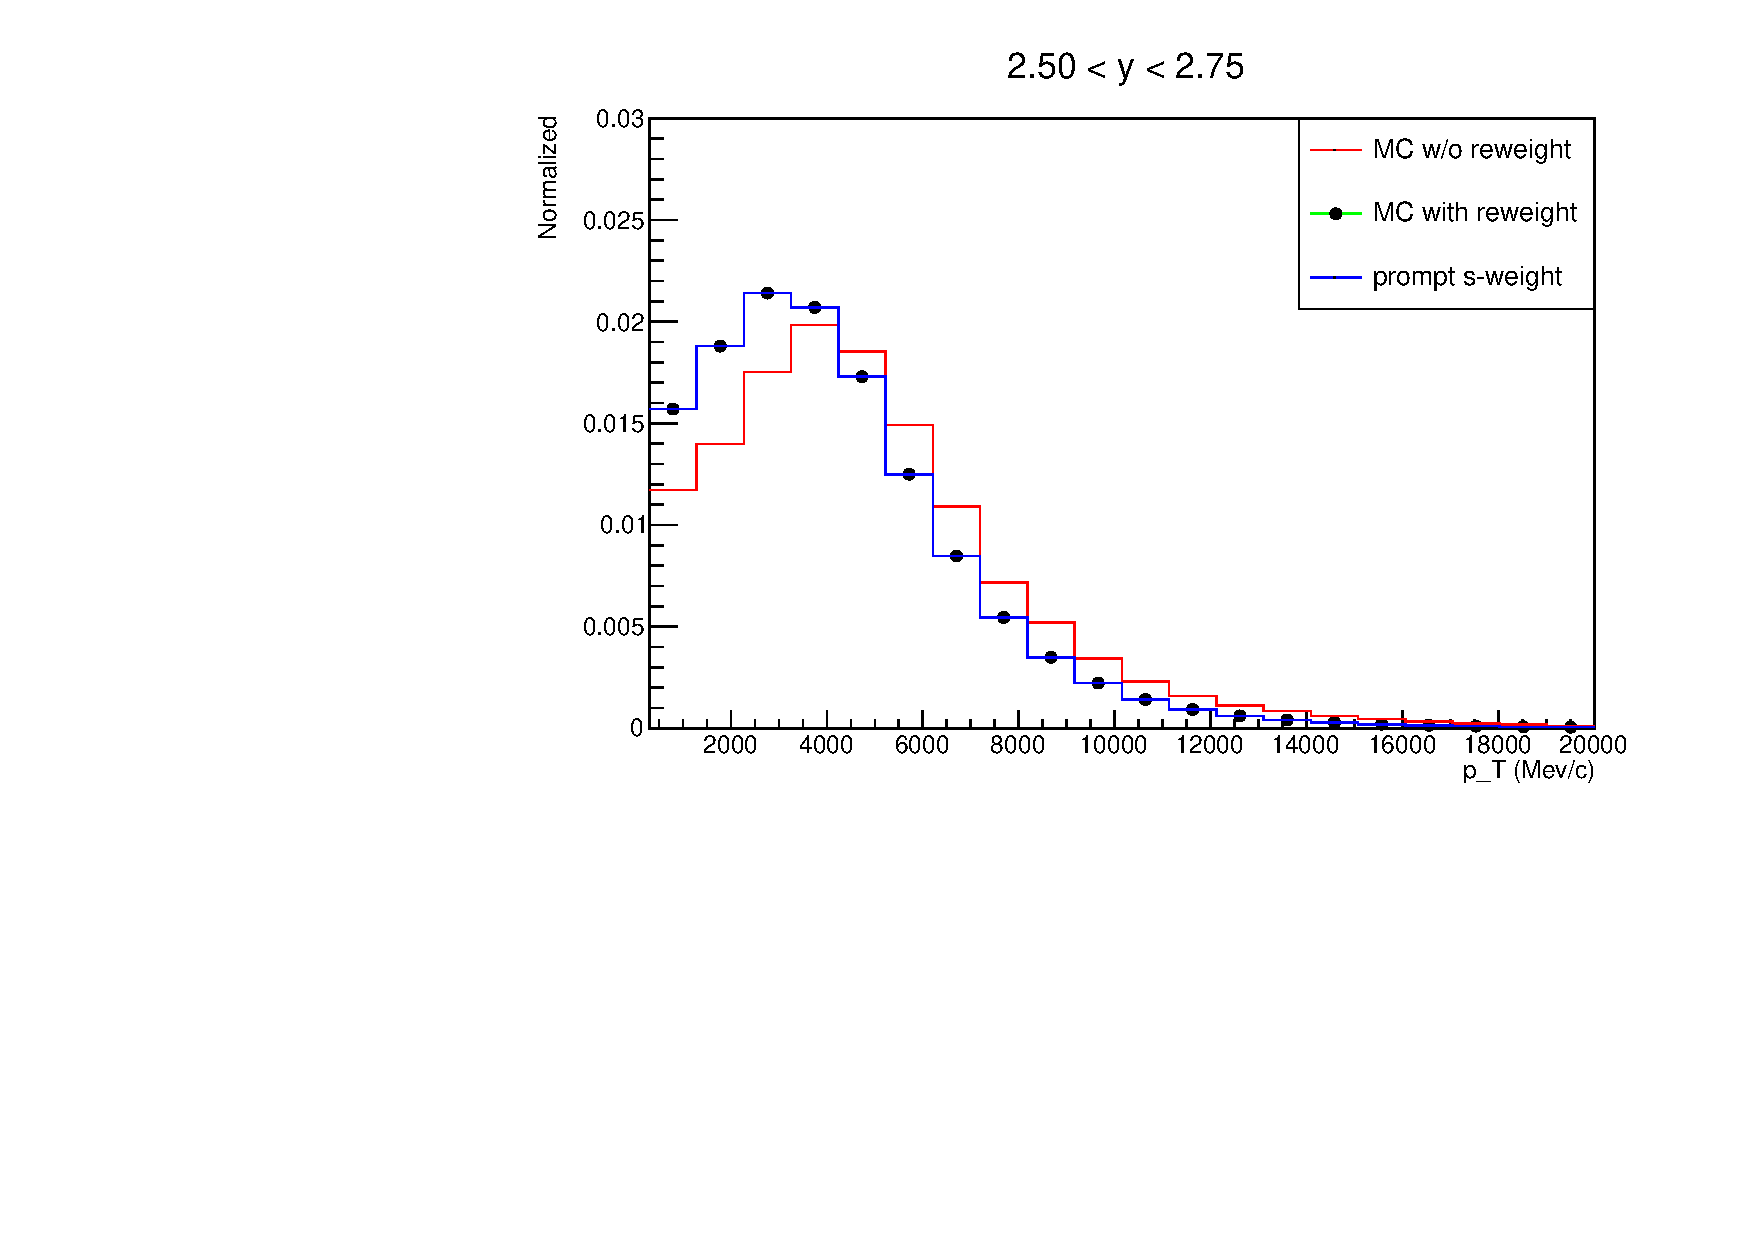
\includegraphics[width=0.19\linewidth]{pdf/Jpsi/reweight/Yp3.pdf}
      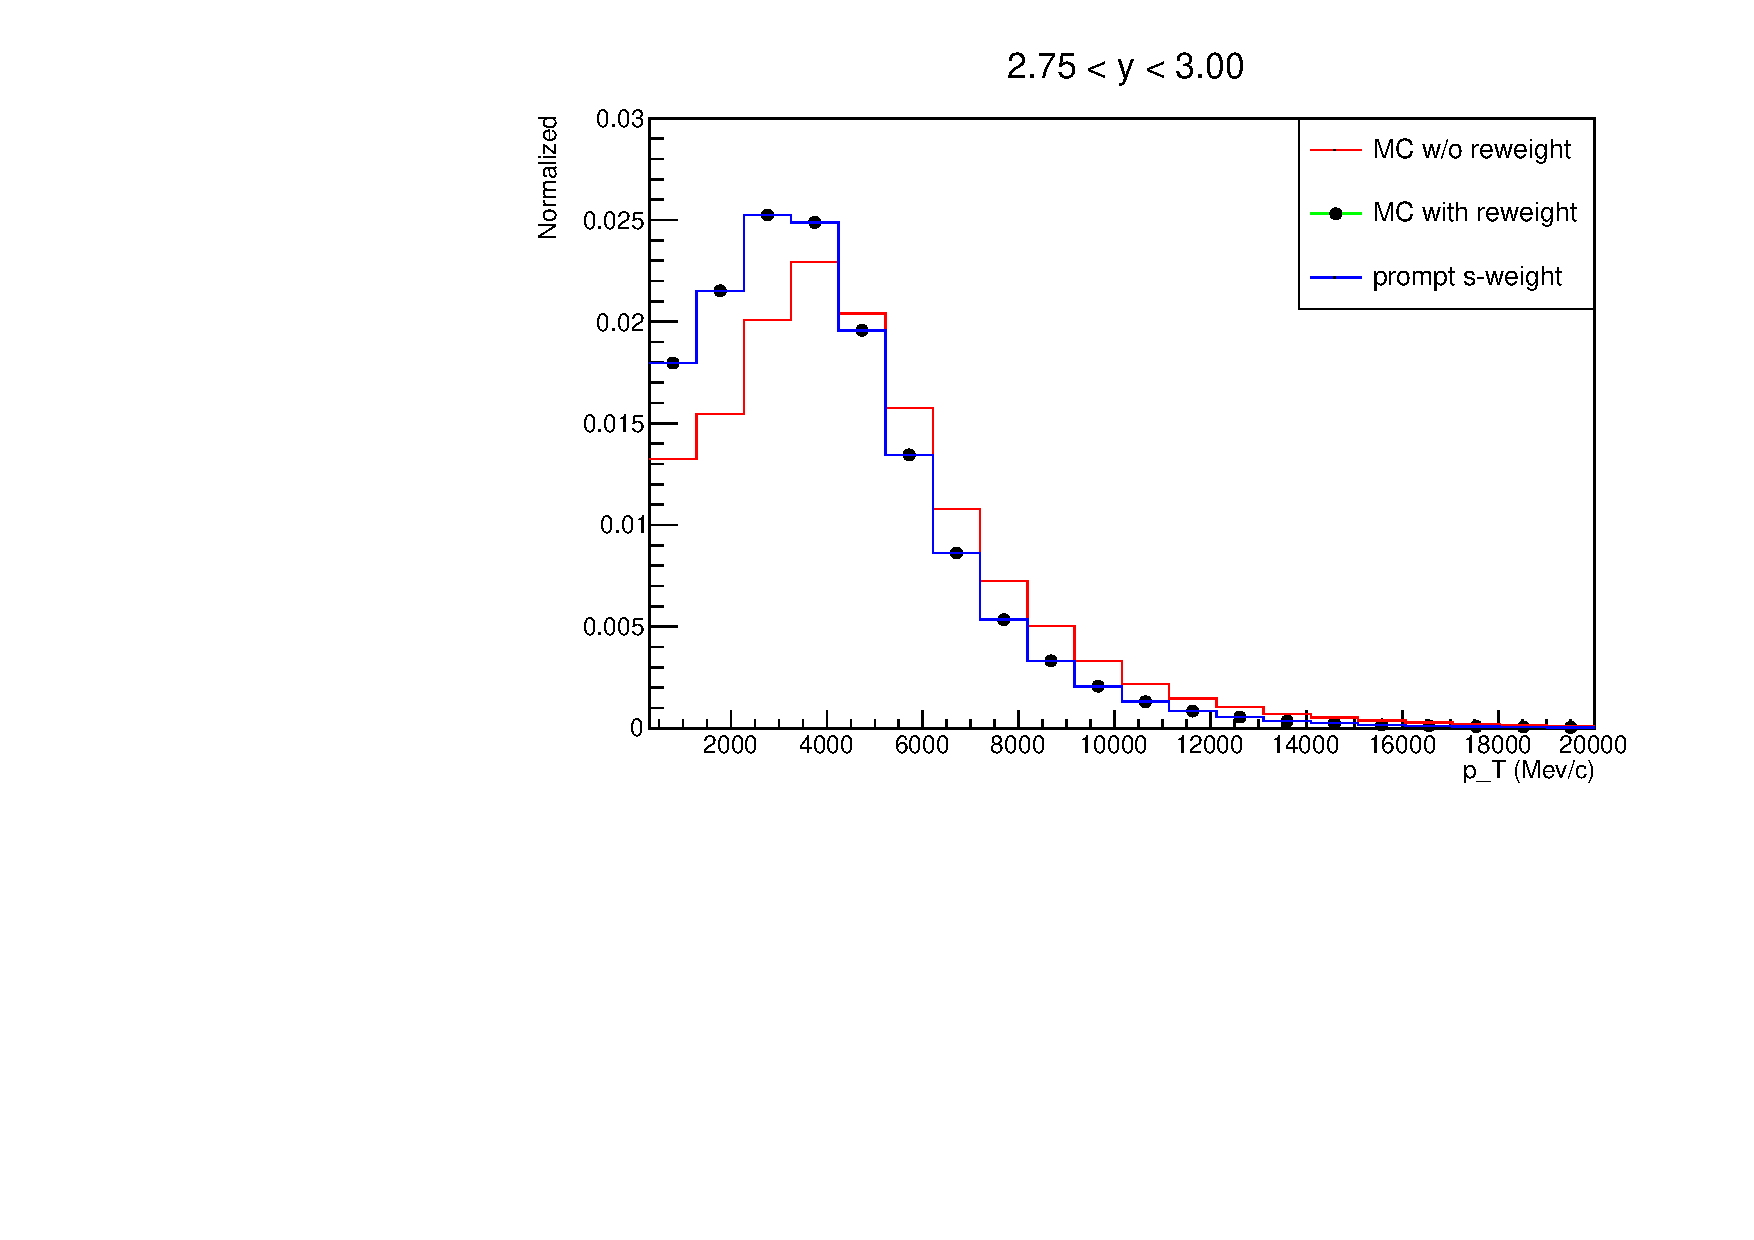
\includegraphics[width=0.19\linewidth]{pdf/Jpsi/reweight/Yp4.pdf}
      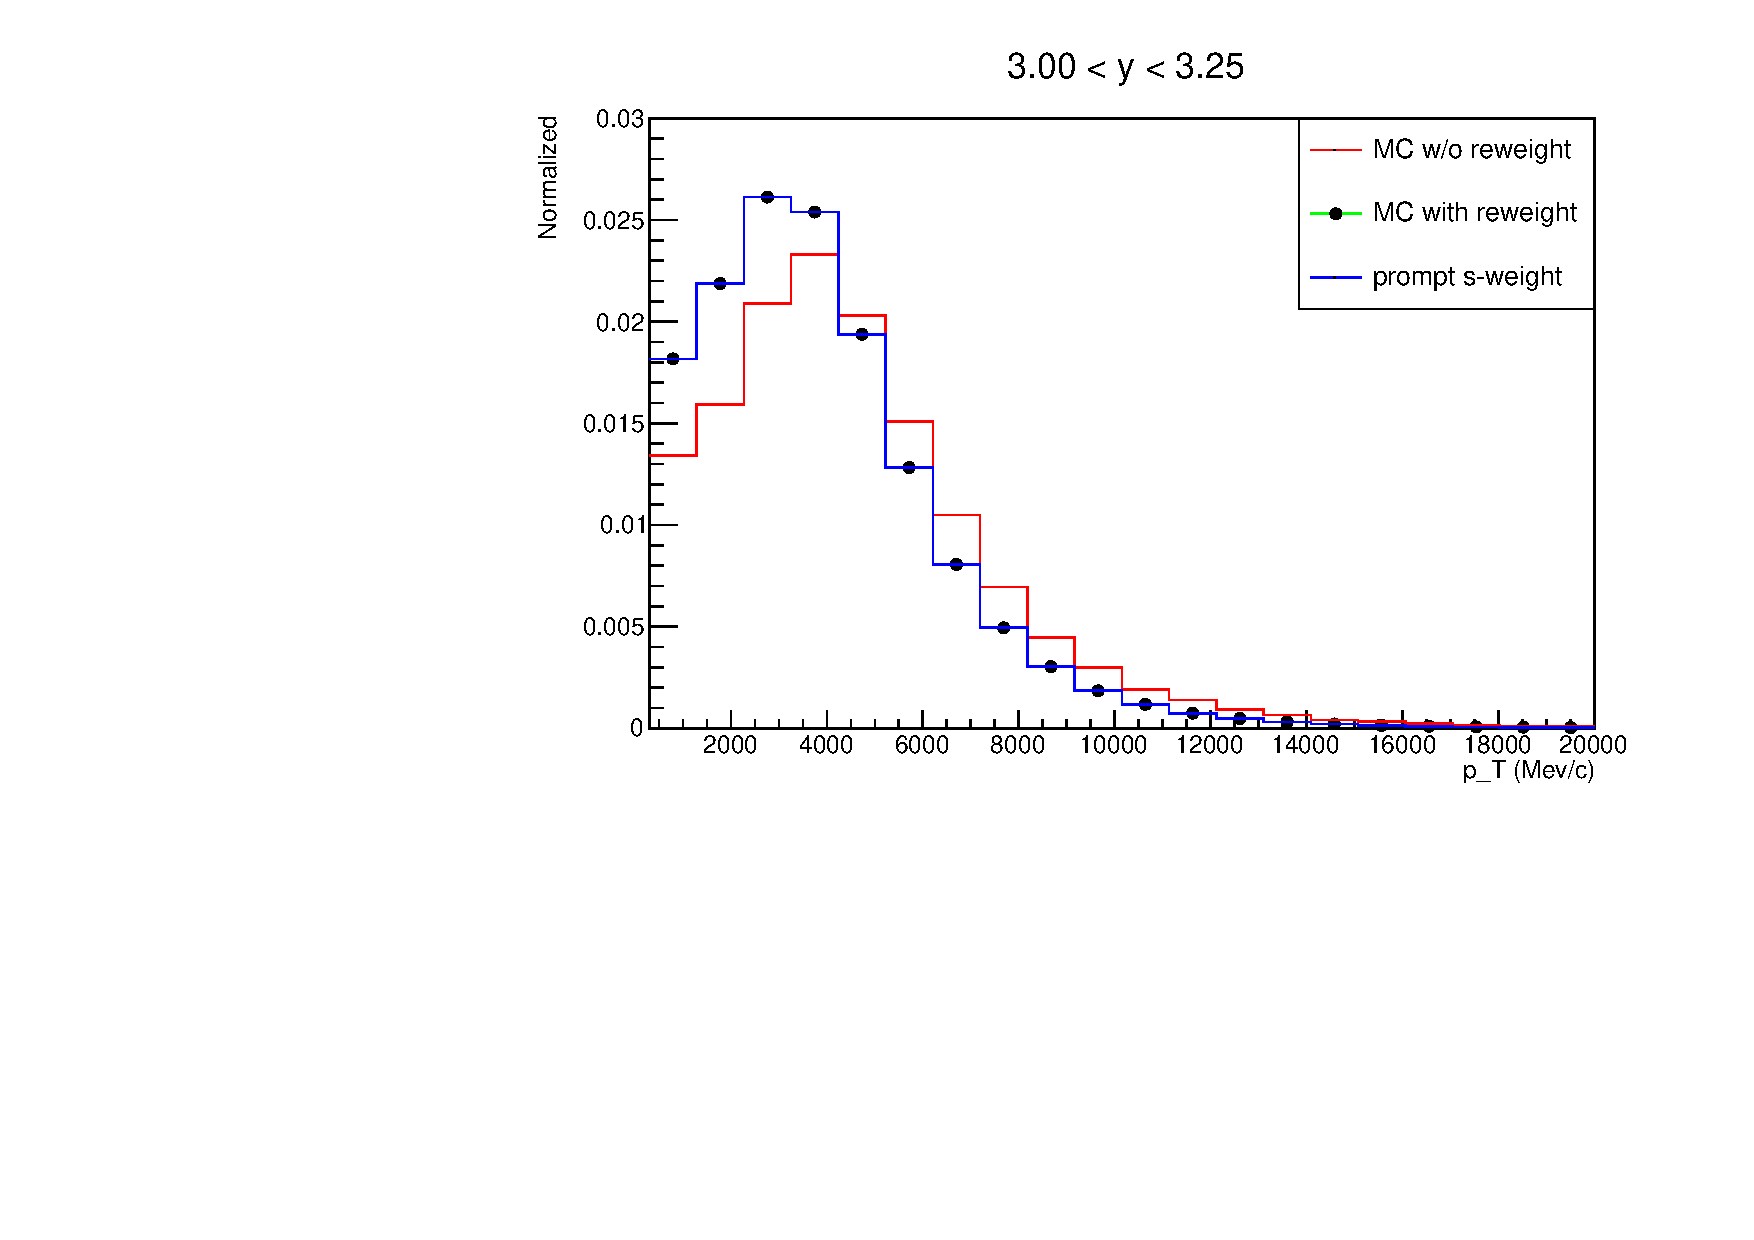
\includegraphics[width=0.19\linewidth]{pdf/Jpsi/reweight/Yp5.pdf}
      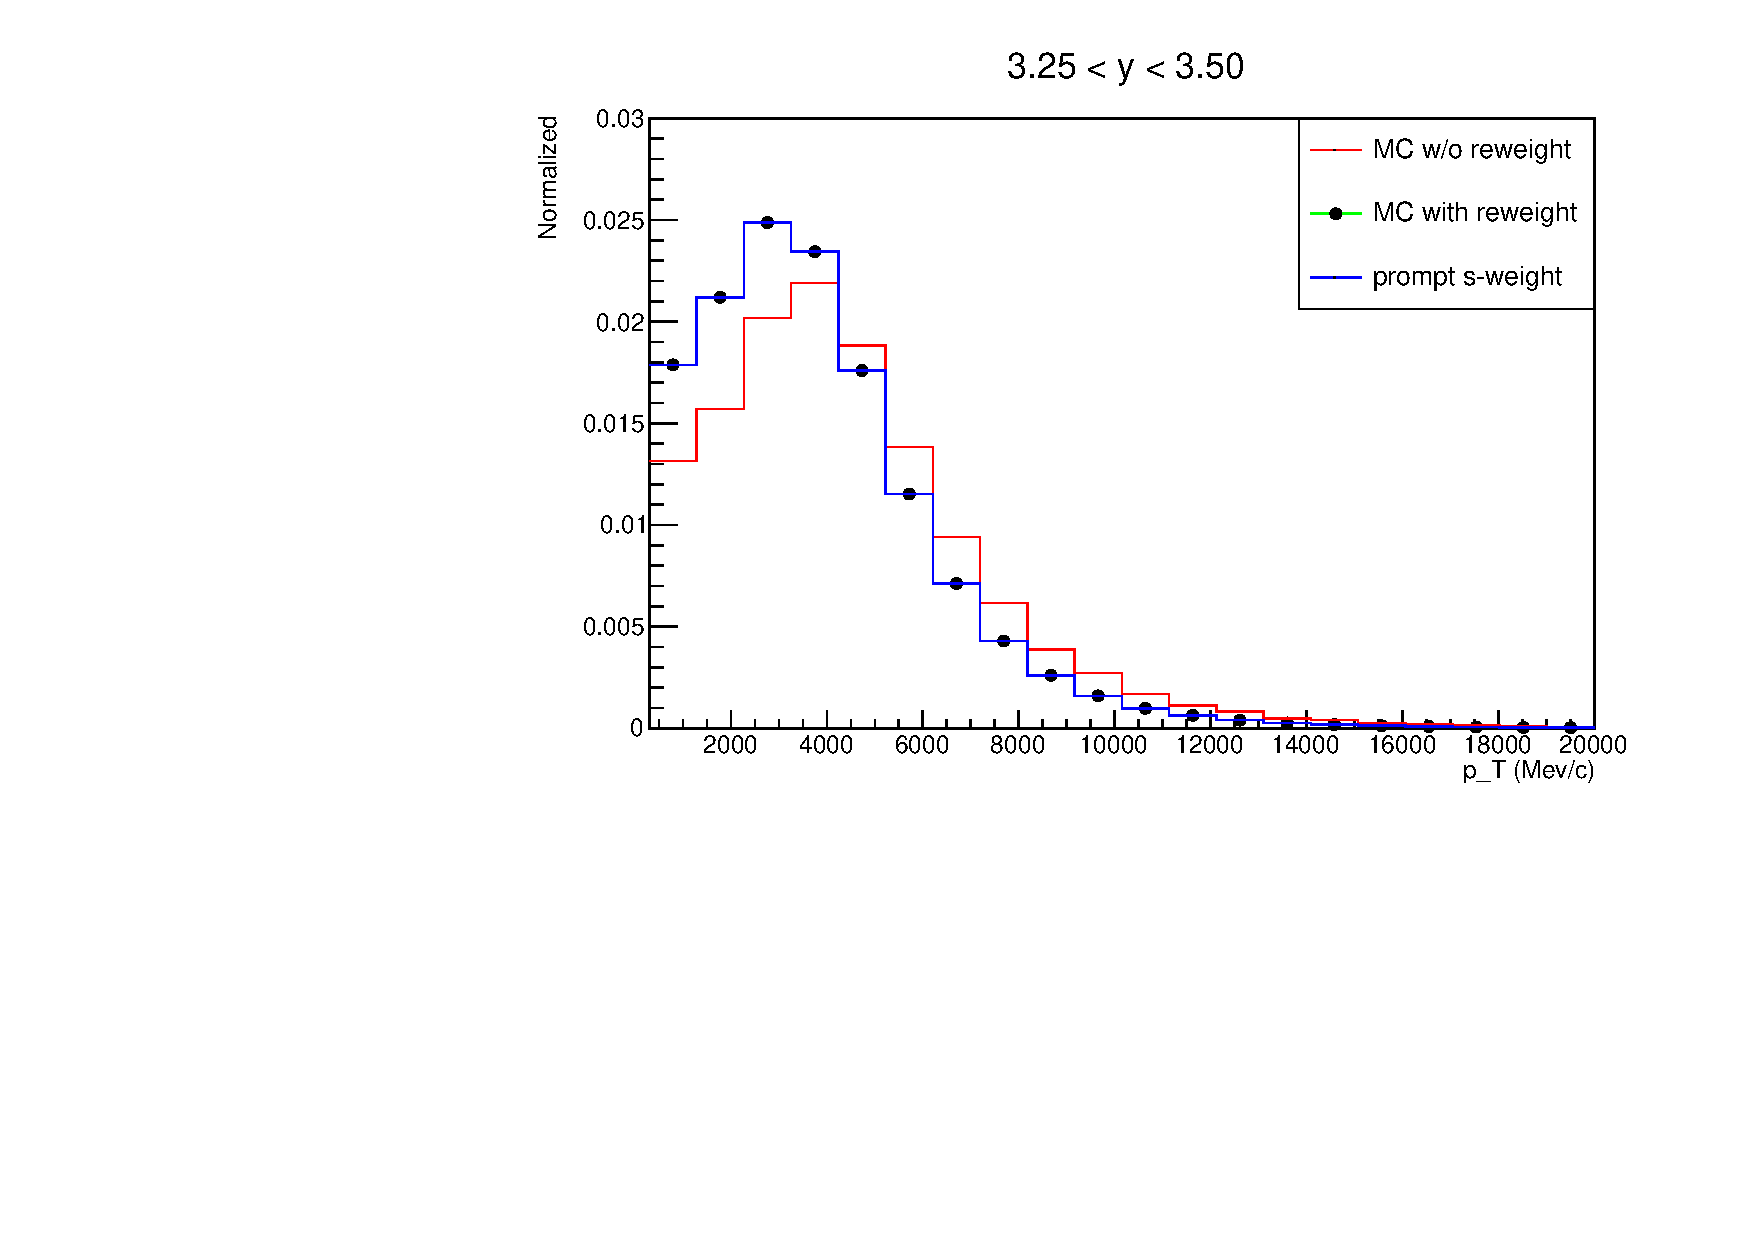
\includegraphics[width=0.19\linewidth]{pdf/Jpsi/reweight/Yp6.pdf}
      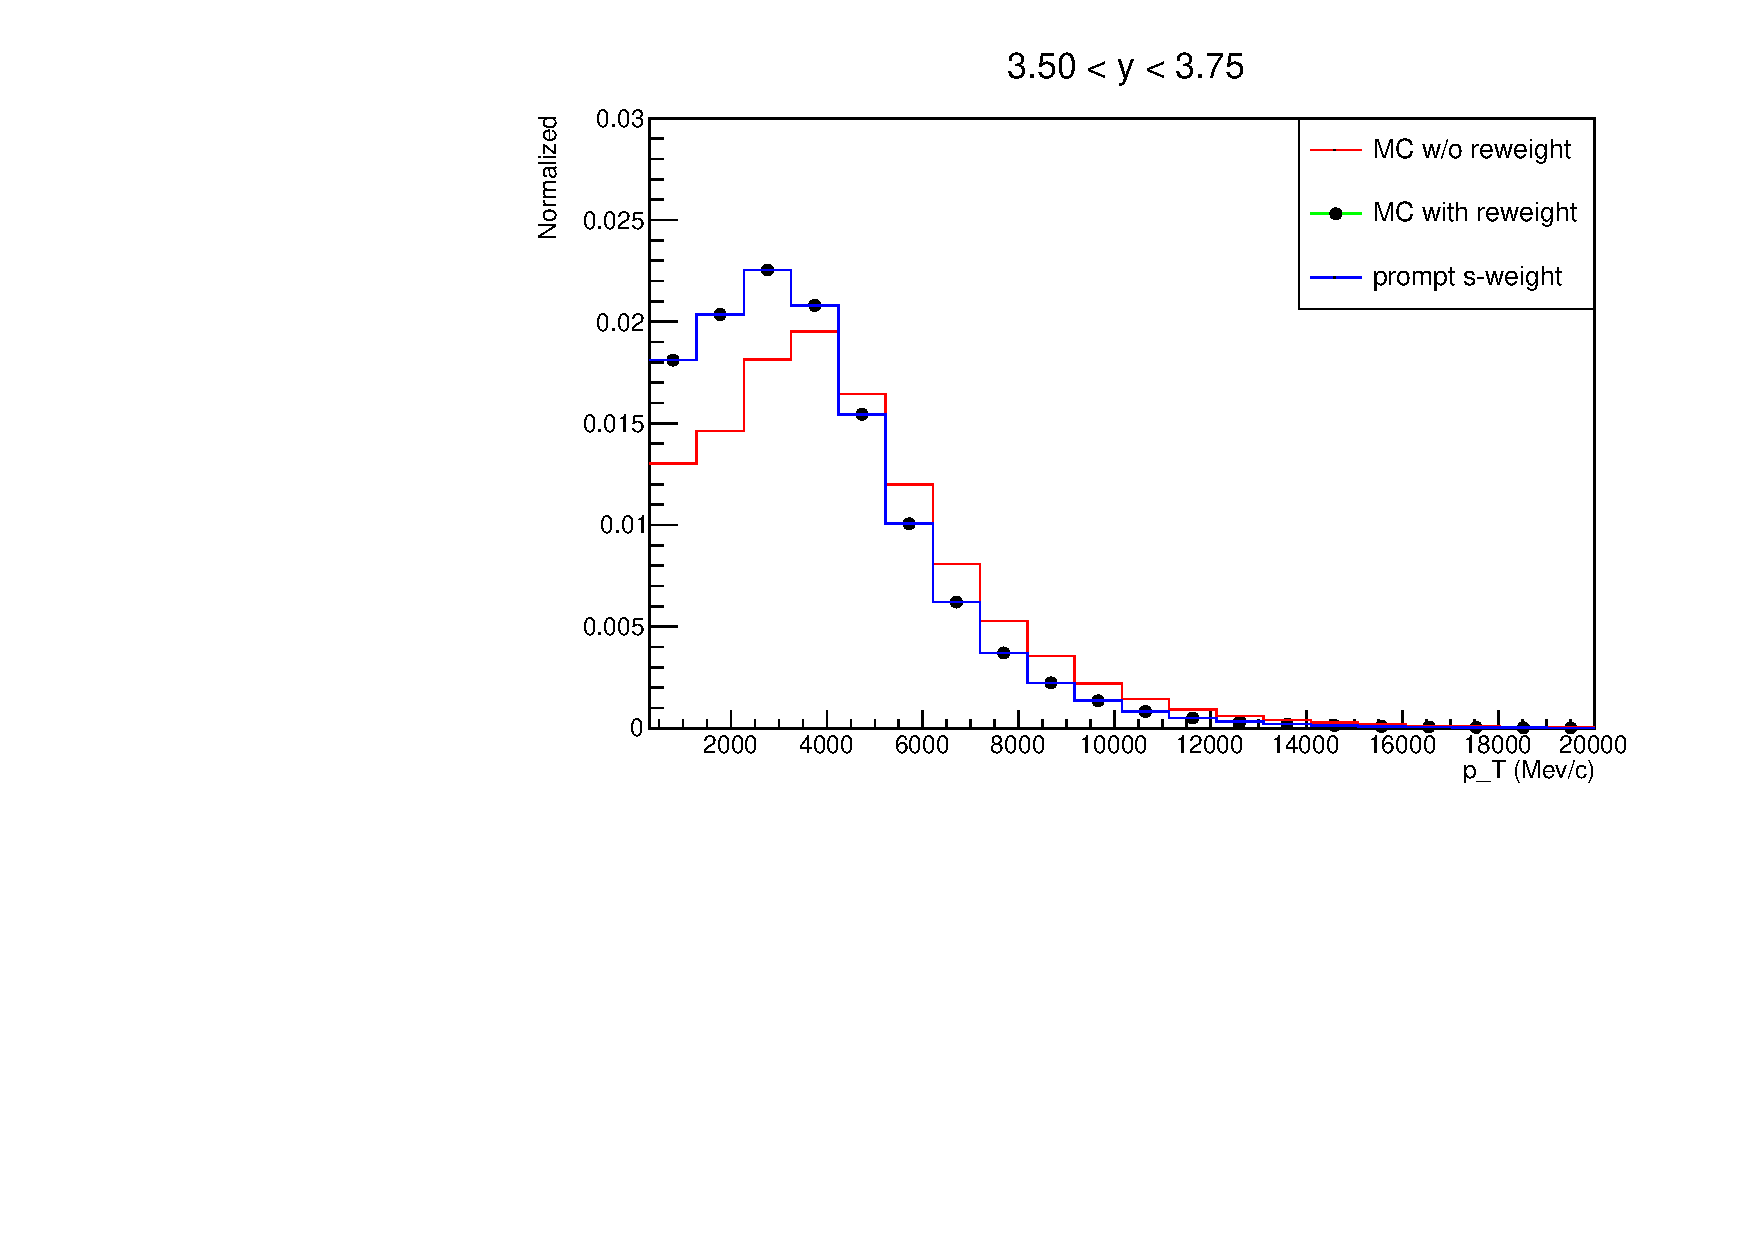
\includegraphics[width=0.19\linewidth]{pdf/Jpsi/reweight/Yp7.pdf}
	  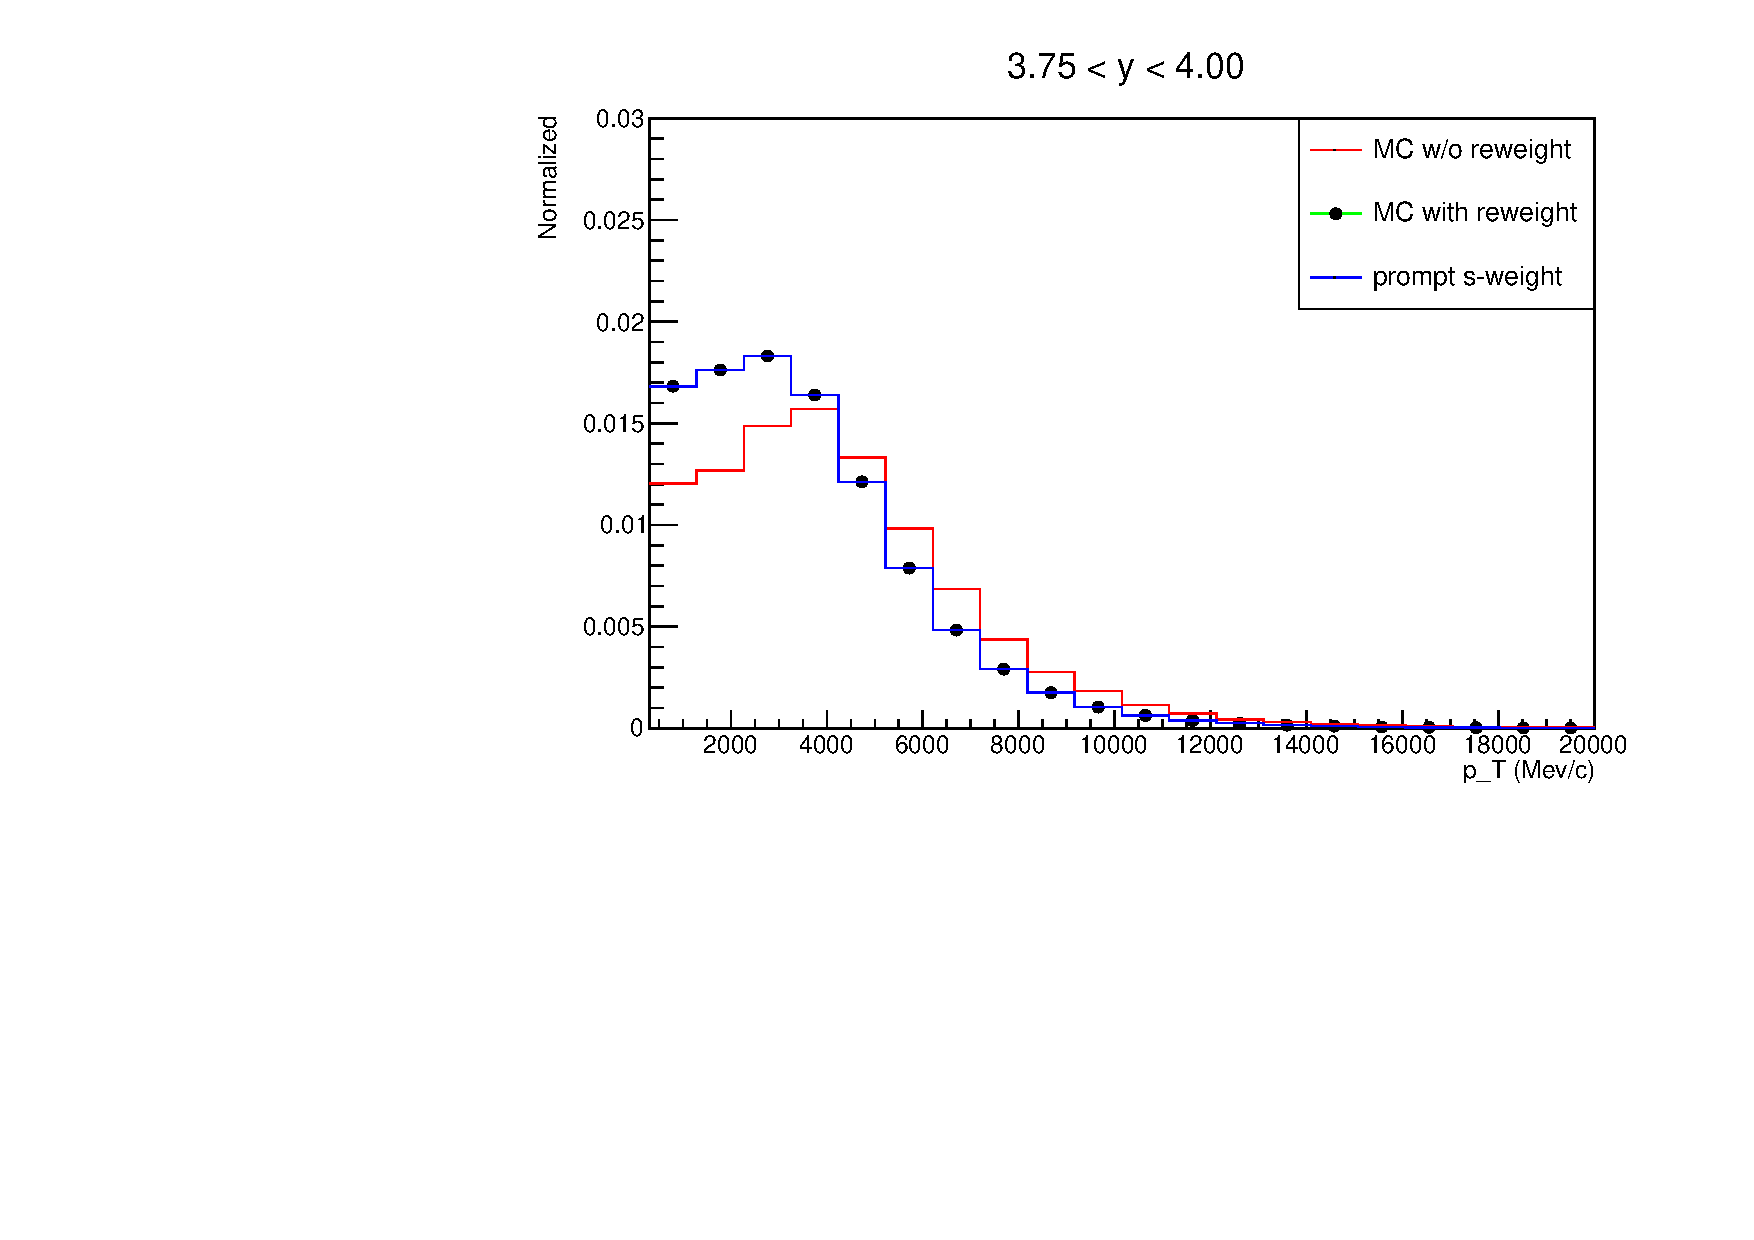
\includegraphics[width=0.19\linewidth]{pdf/Jpsi/reweight/Yp8.pdf}
      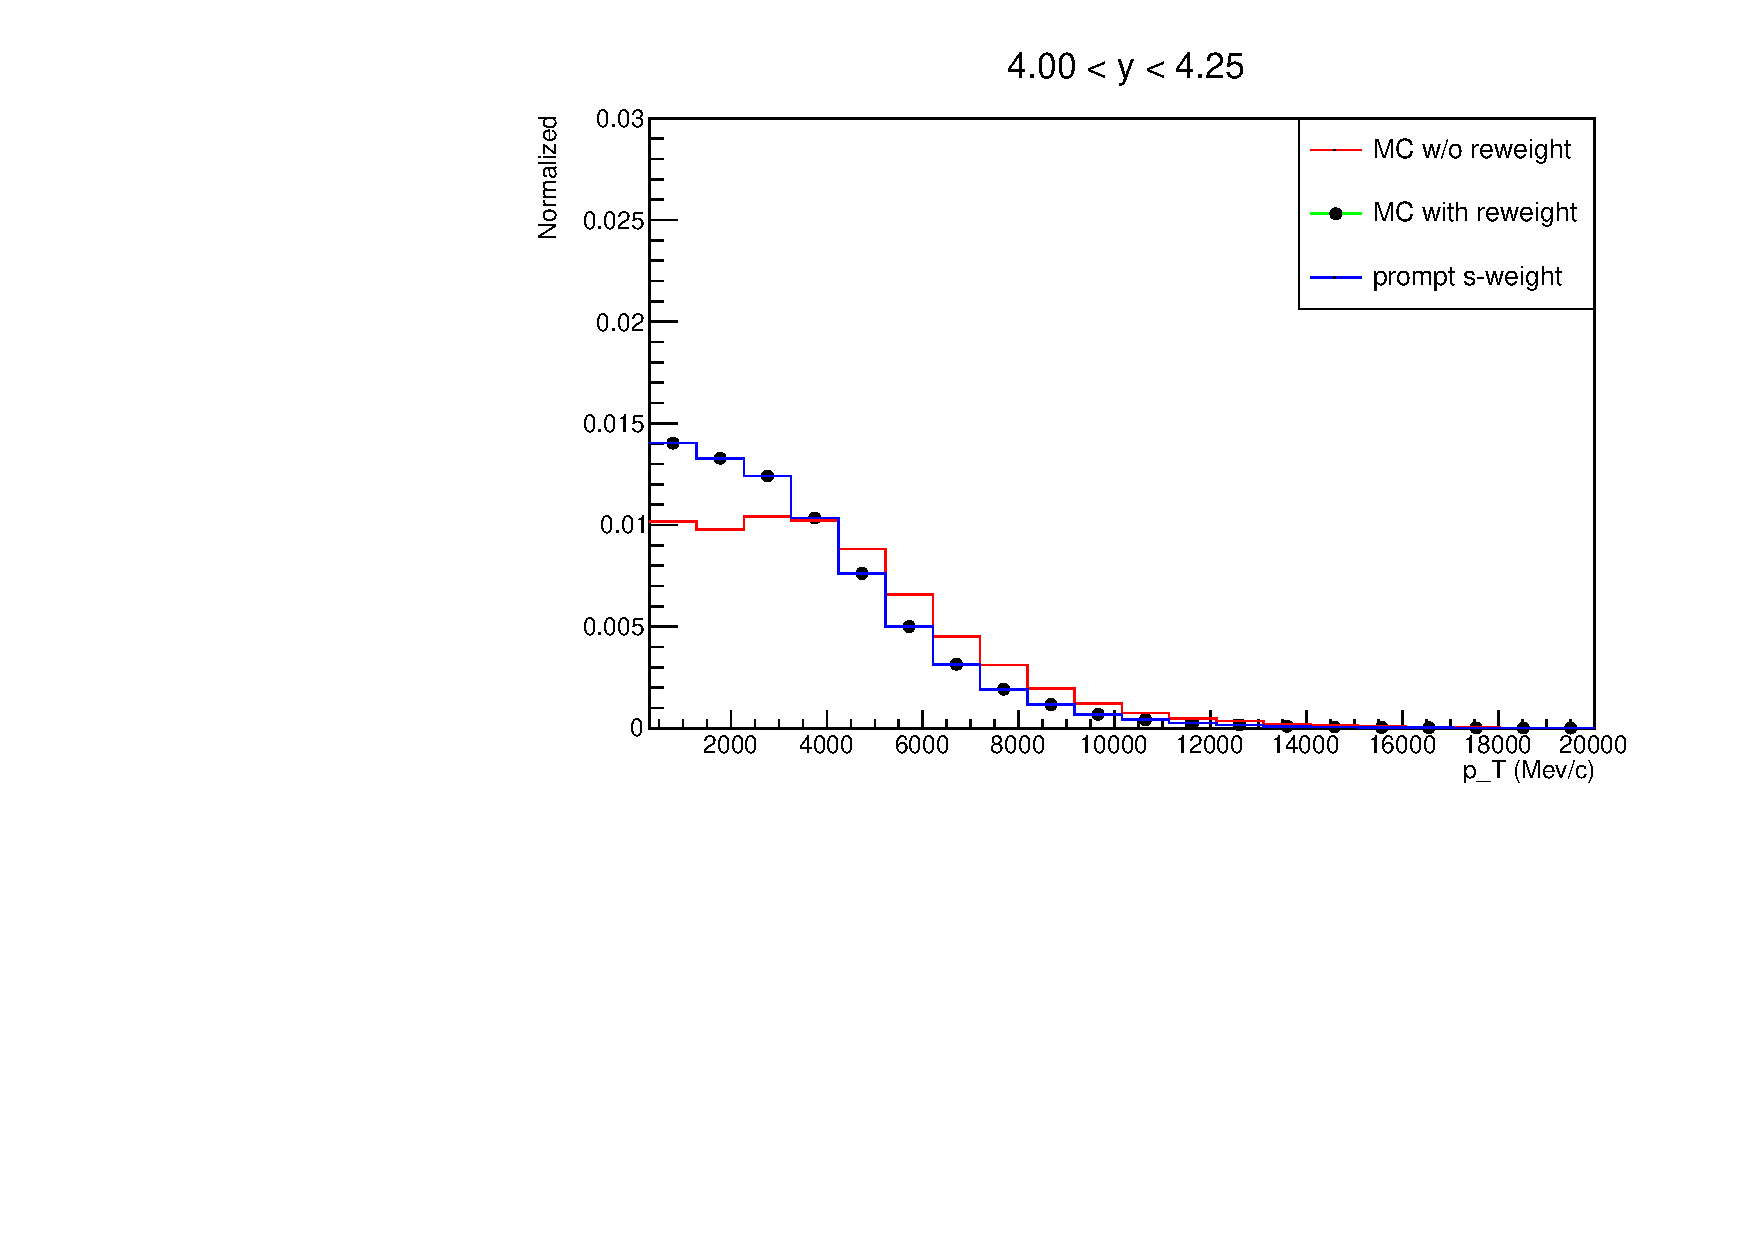
\includegraphics[width=0.19\linewidth]{pdf/Jpsi/reweight/Yp9.pdf}
      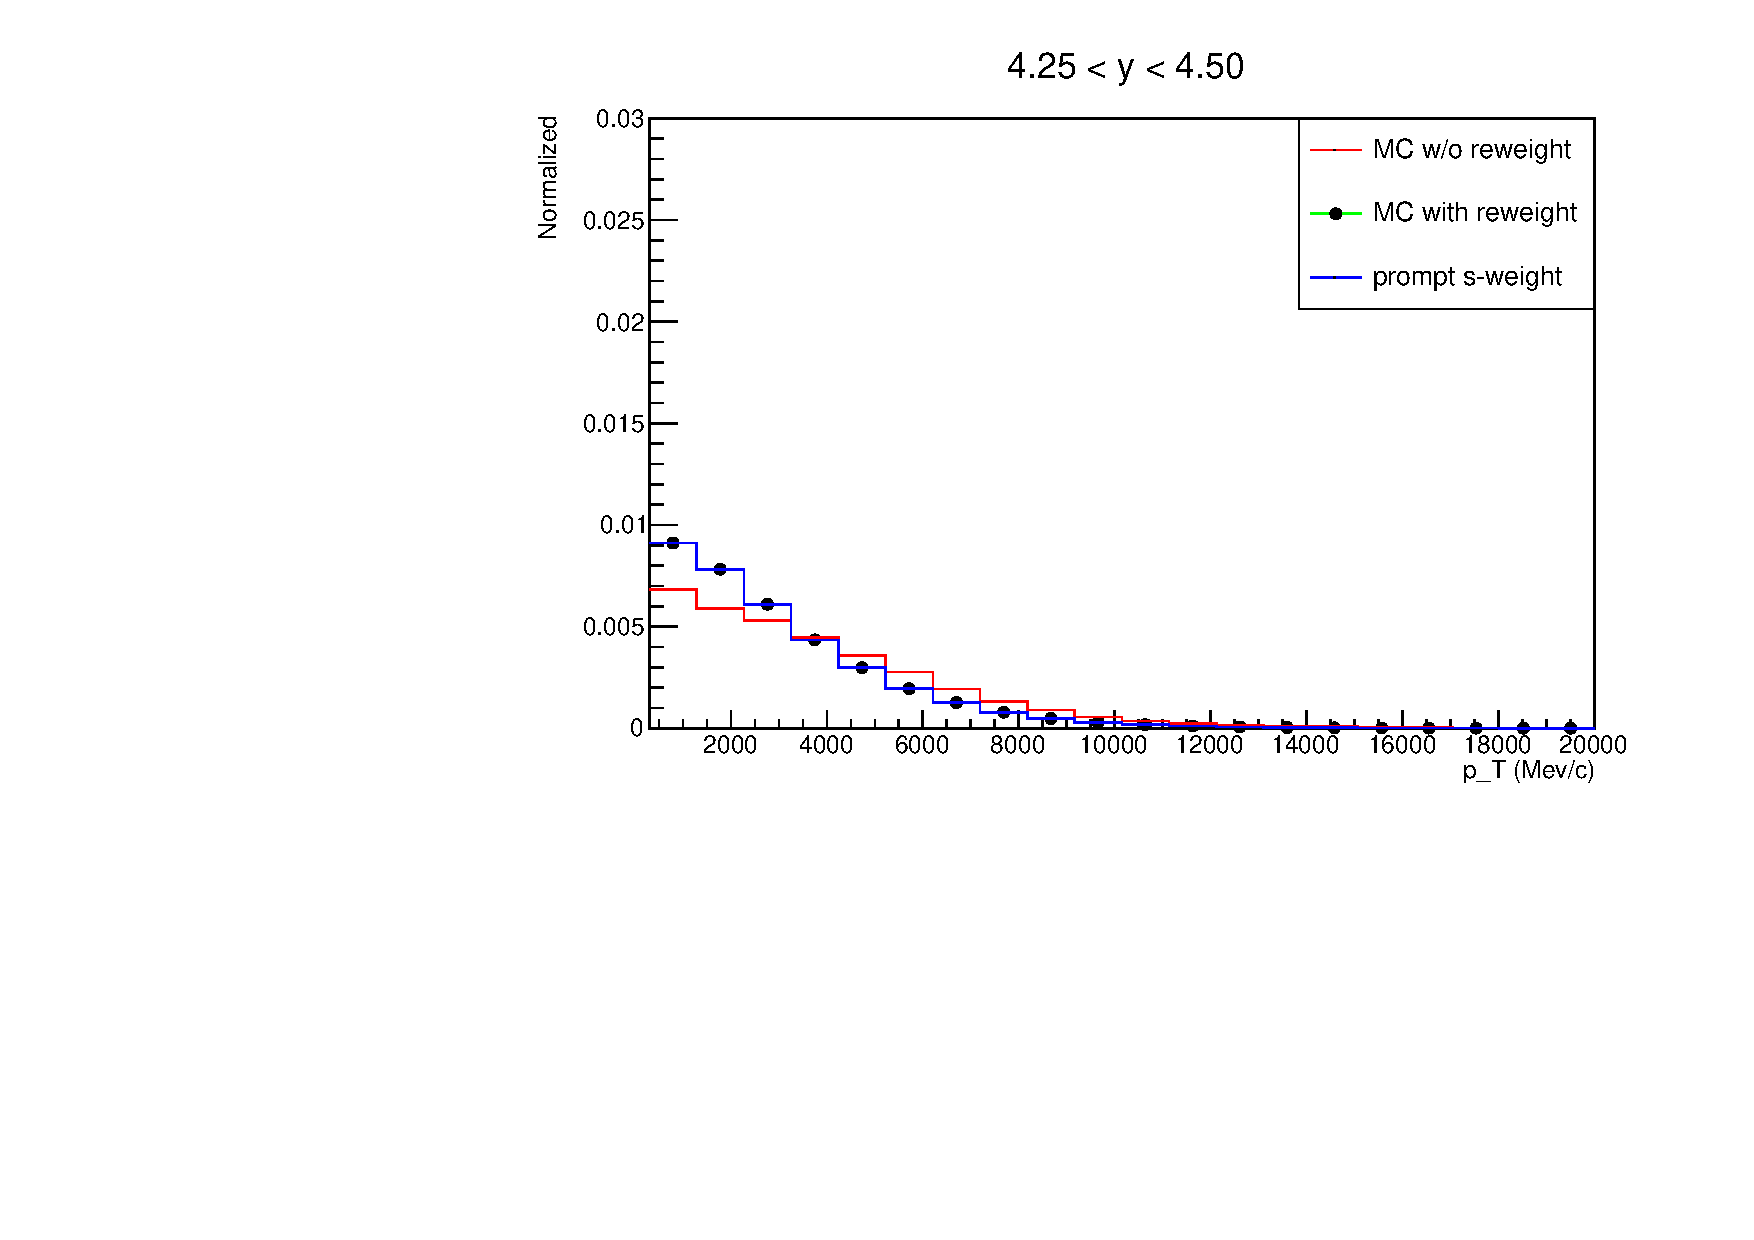
\includegraphics[width=0.19\linewidth]{pdf/Jpsi/reweight/Yp10.pdf}
	  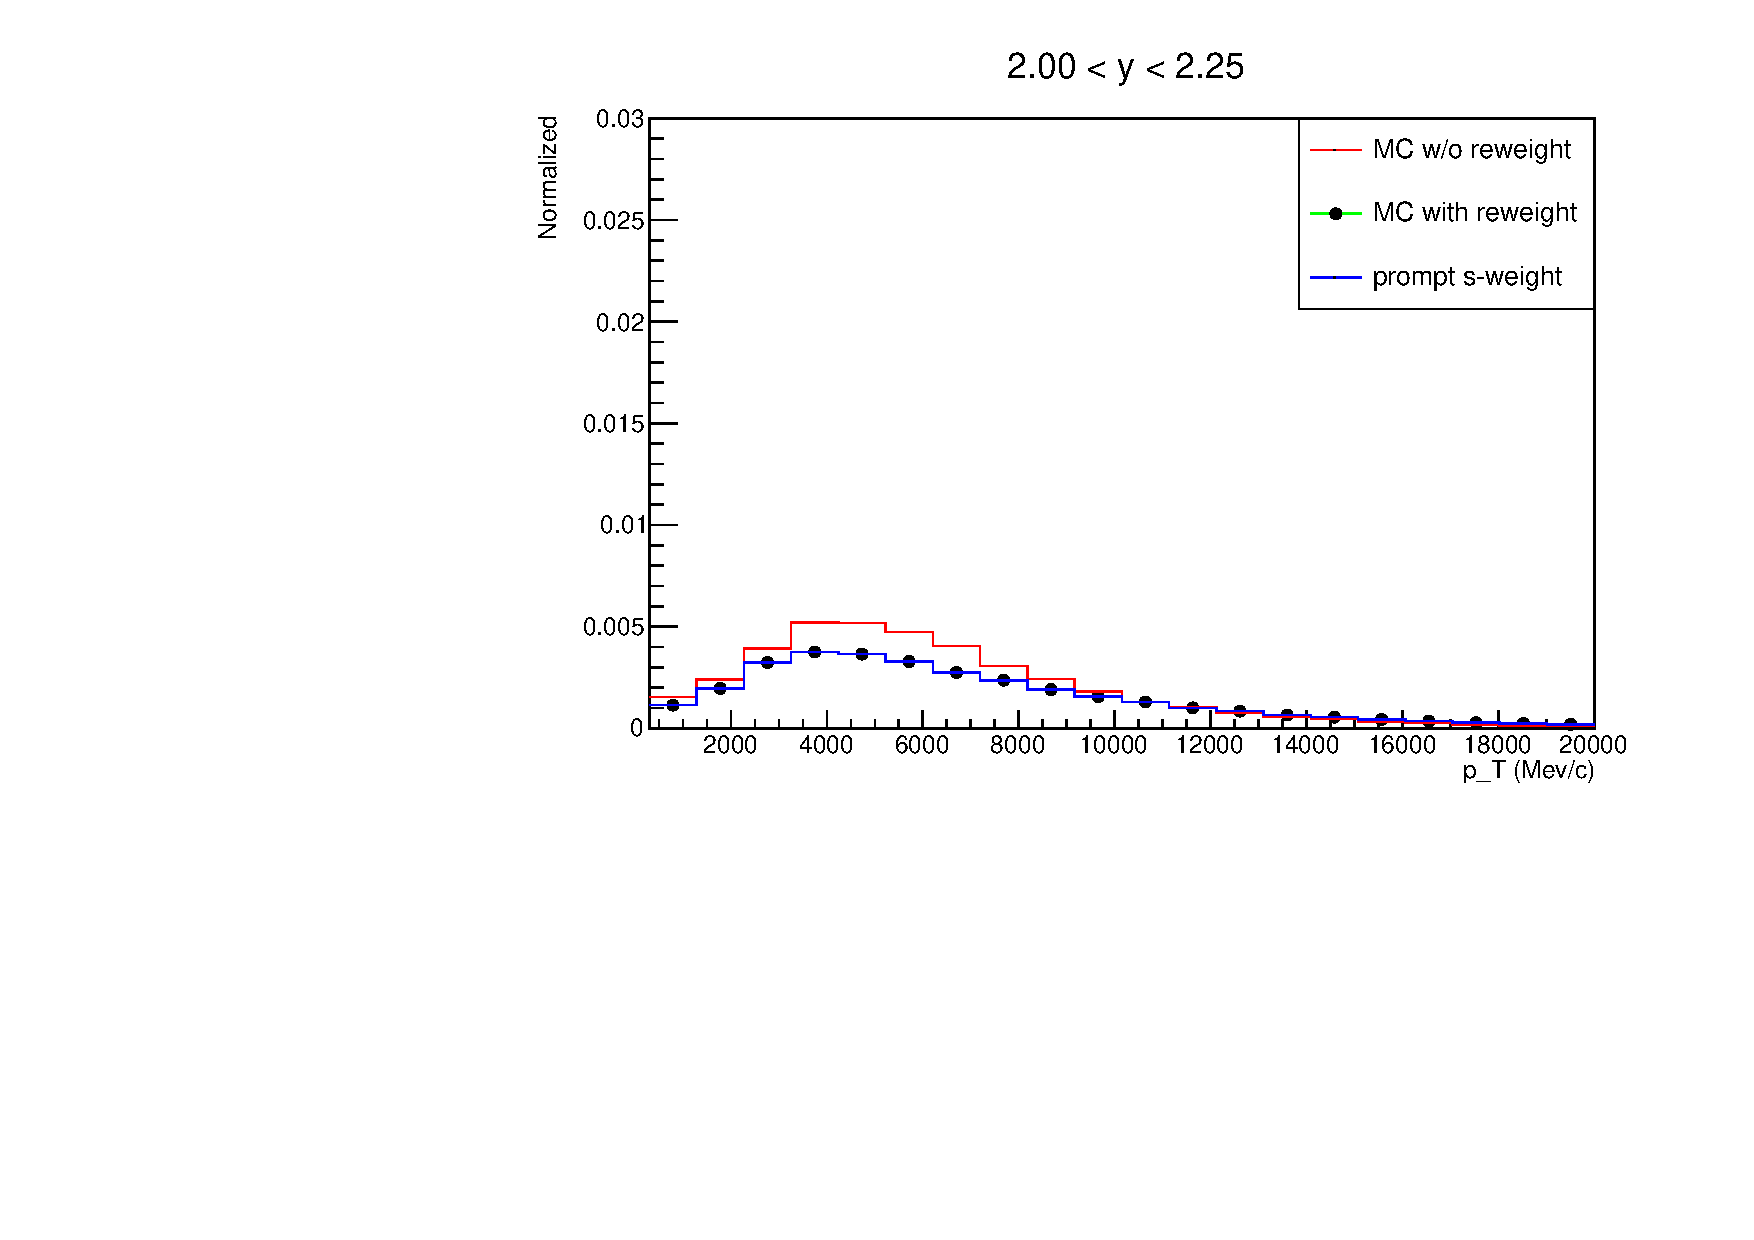
\includegraphics[width=0.19\linewidth]{pdf/Jpsi/reweight/Yb1.pdf}
      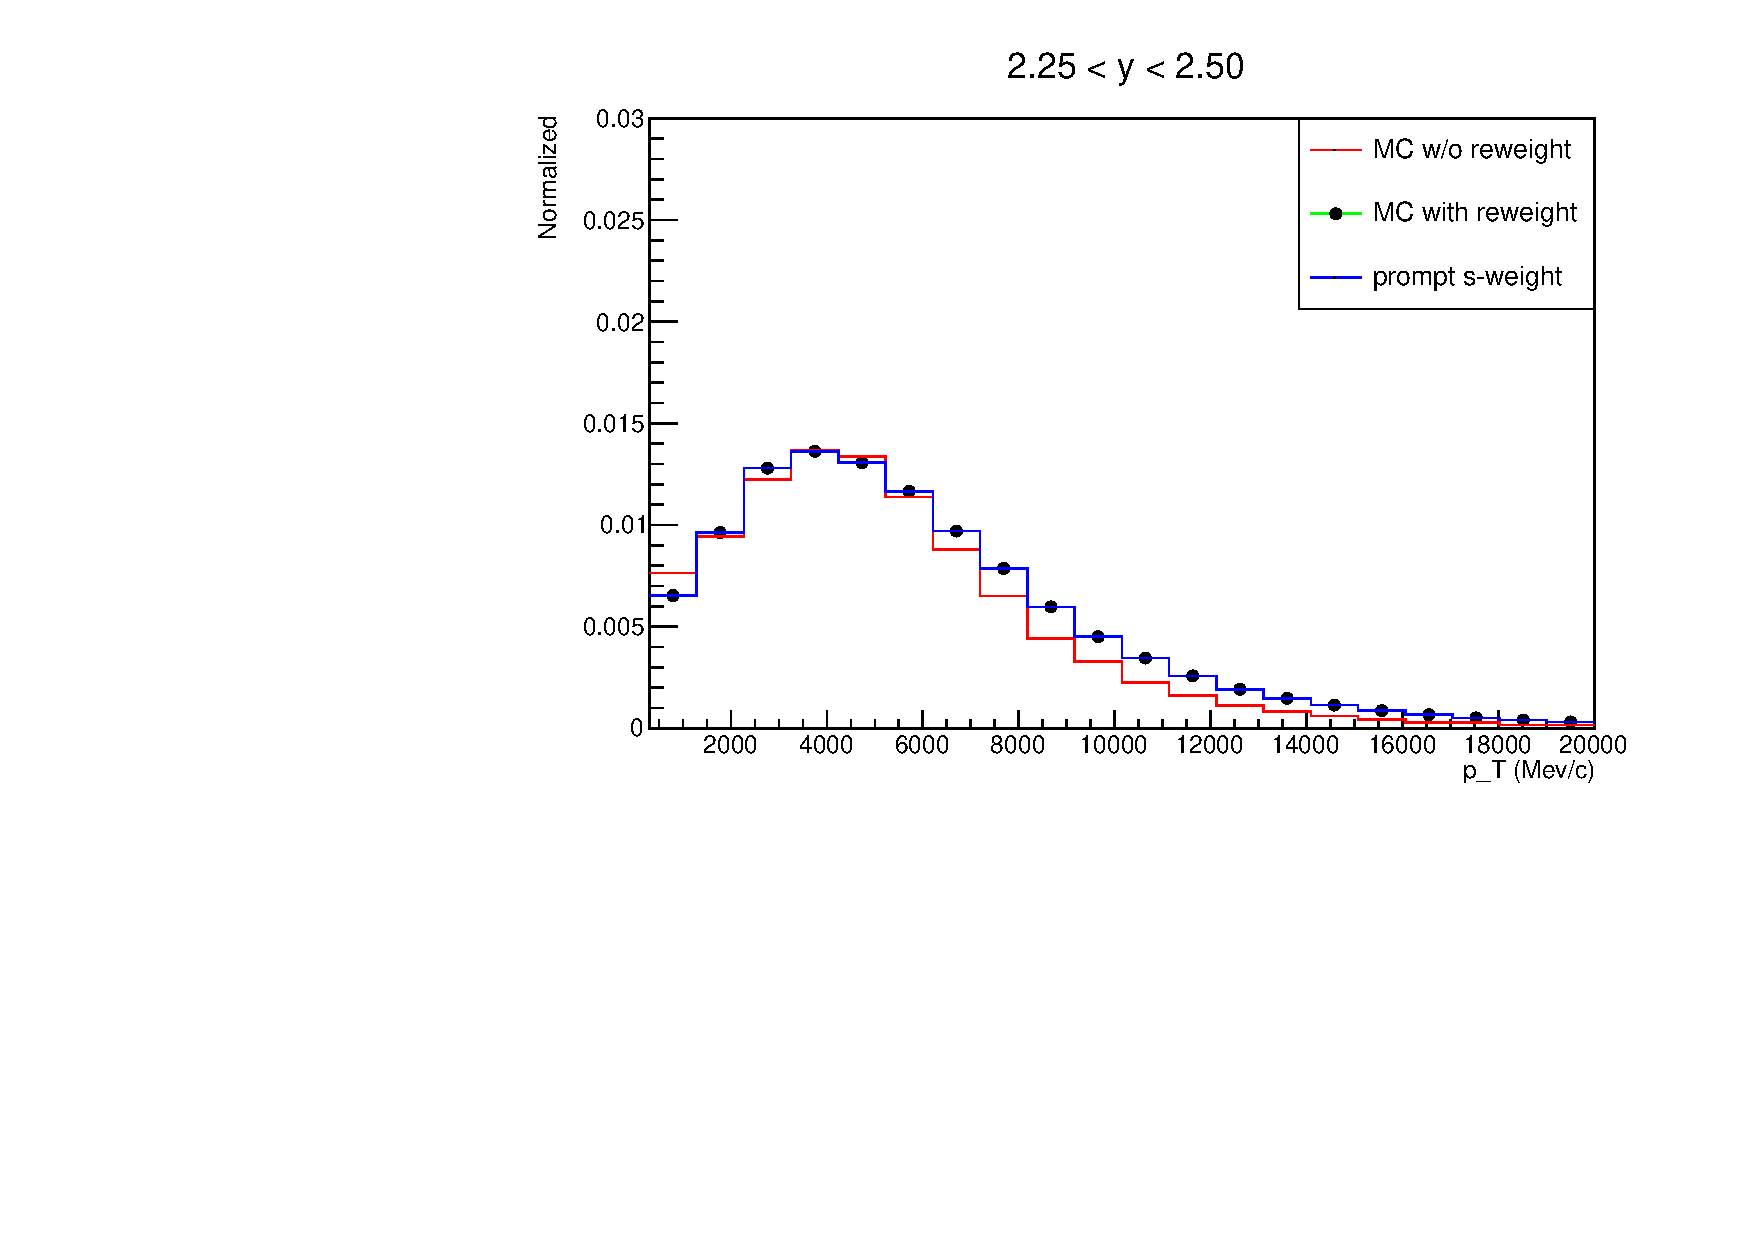
\includegraphics[width=0.19\linewidth]{pdf/Jpsi/reweight/Yb2.pdf} 
      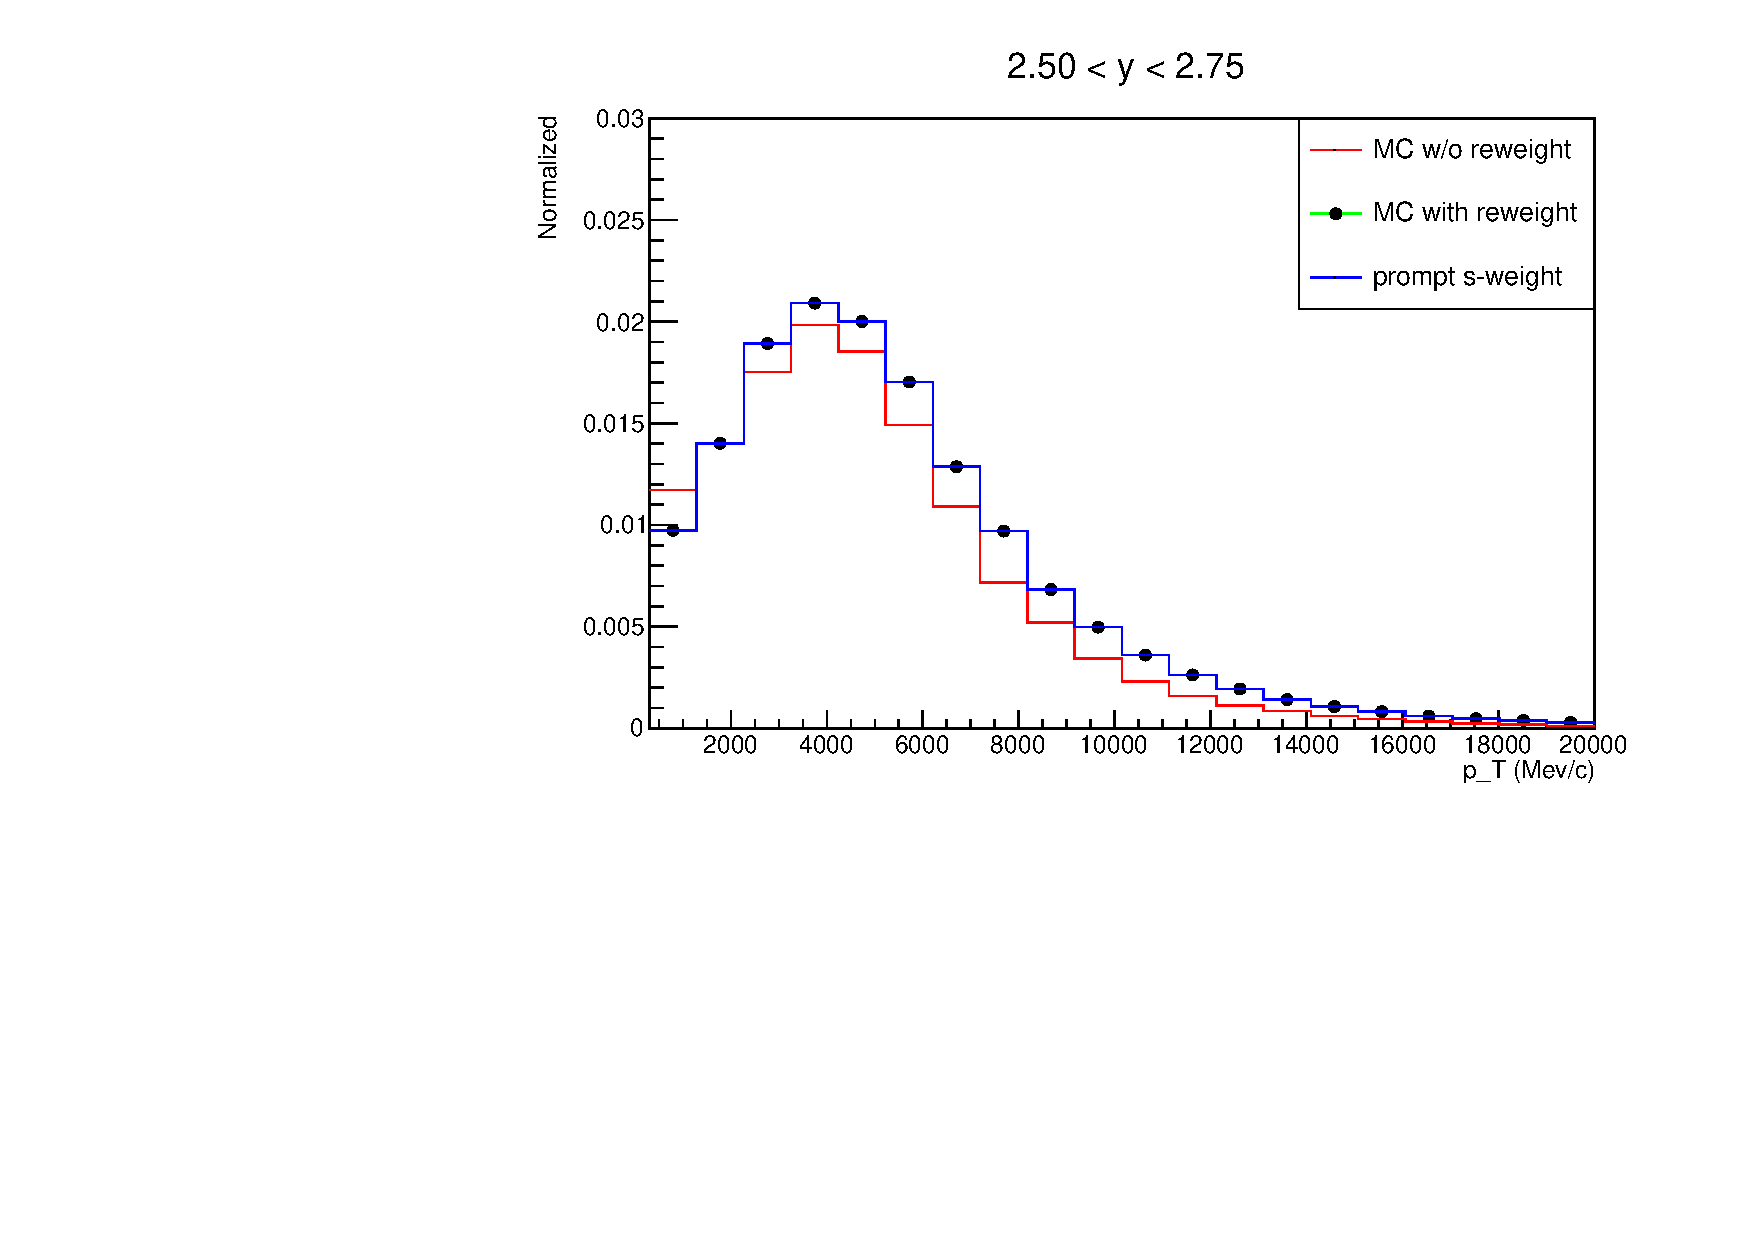
\includegraphics[width=0.19\linewidth]{pdf/Jpsi/reweight/Yb3.pdf}
      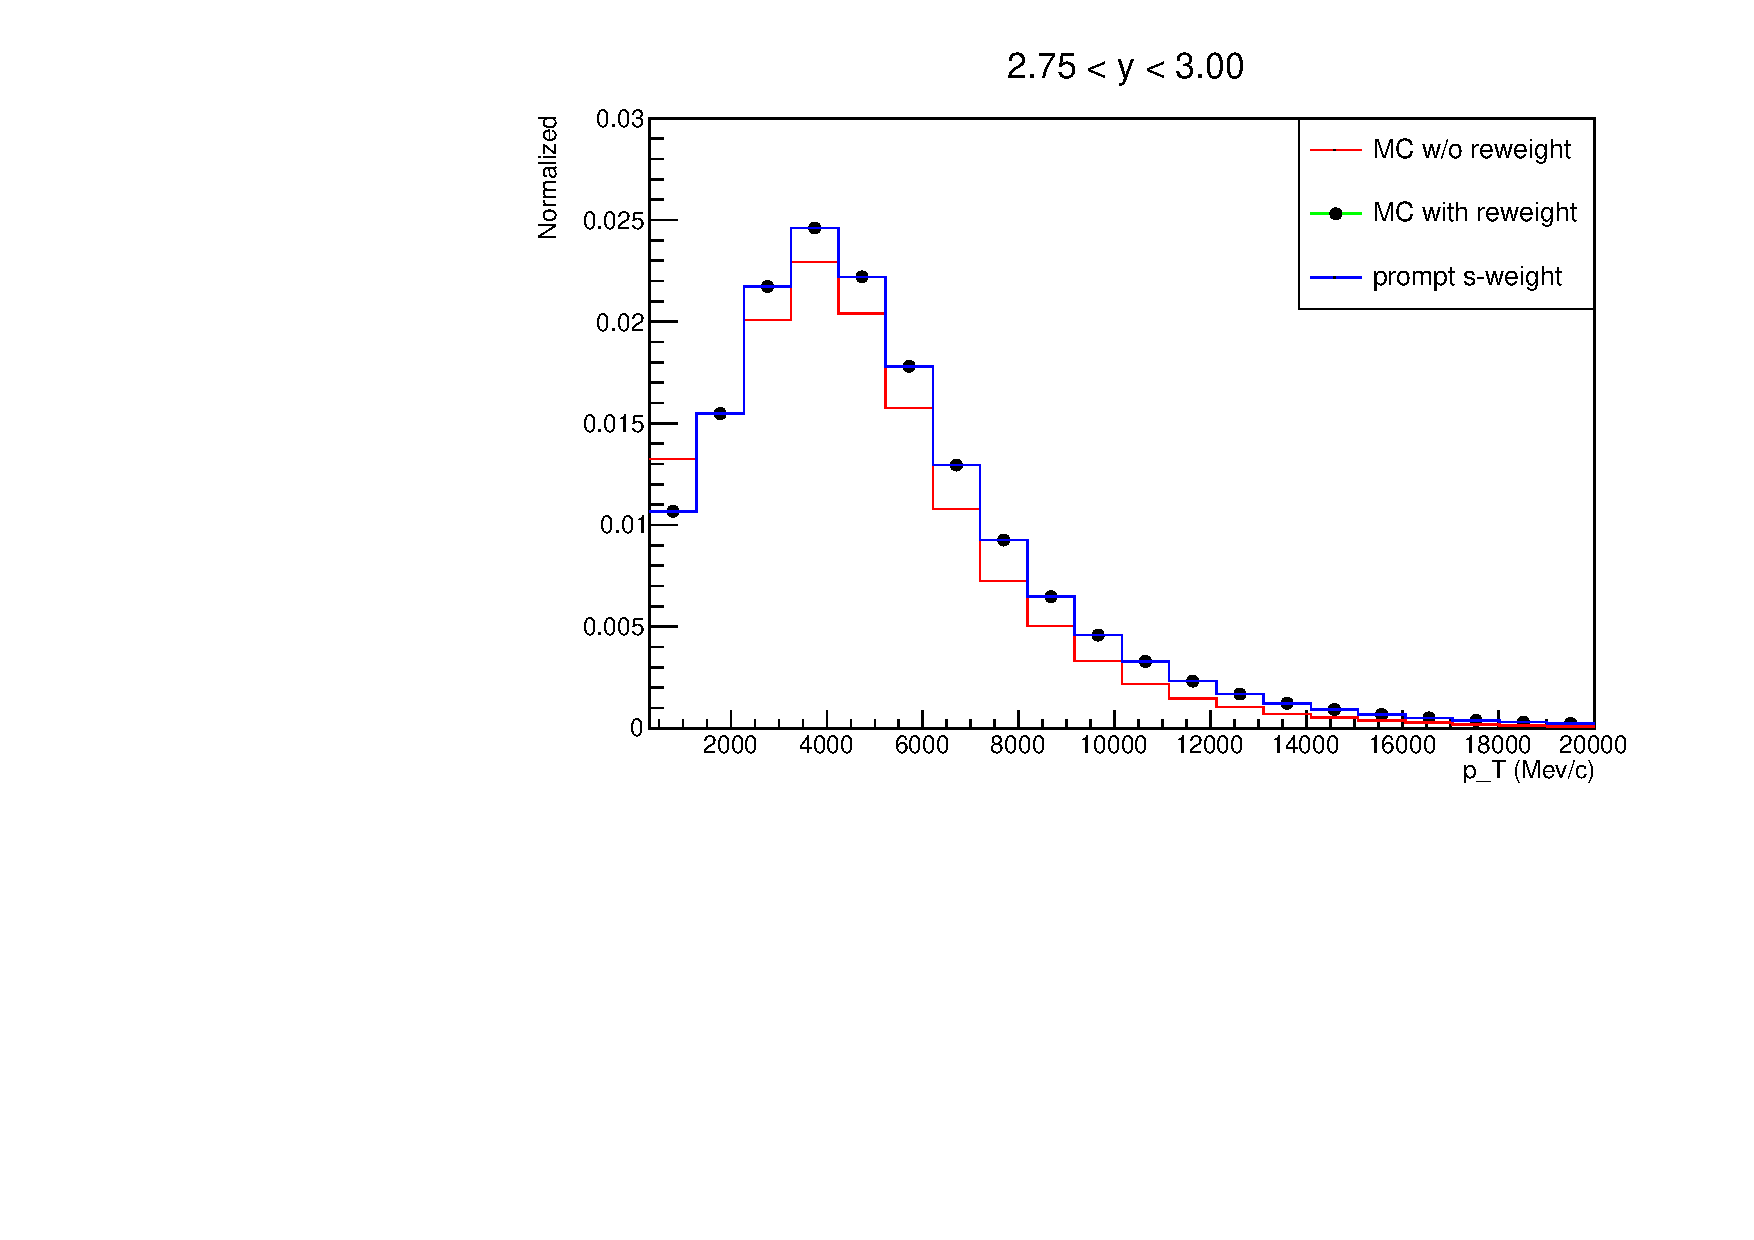
\includegraphics[width=0.19\linewidth]{pdf/Jpsi/reweight/Yb4.pdf}
      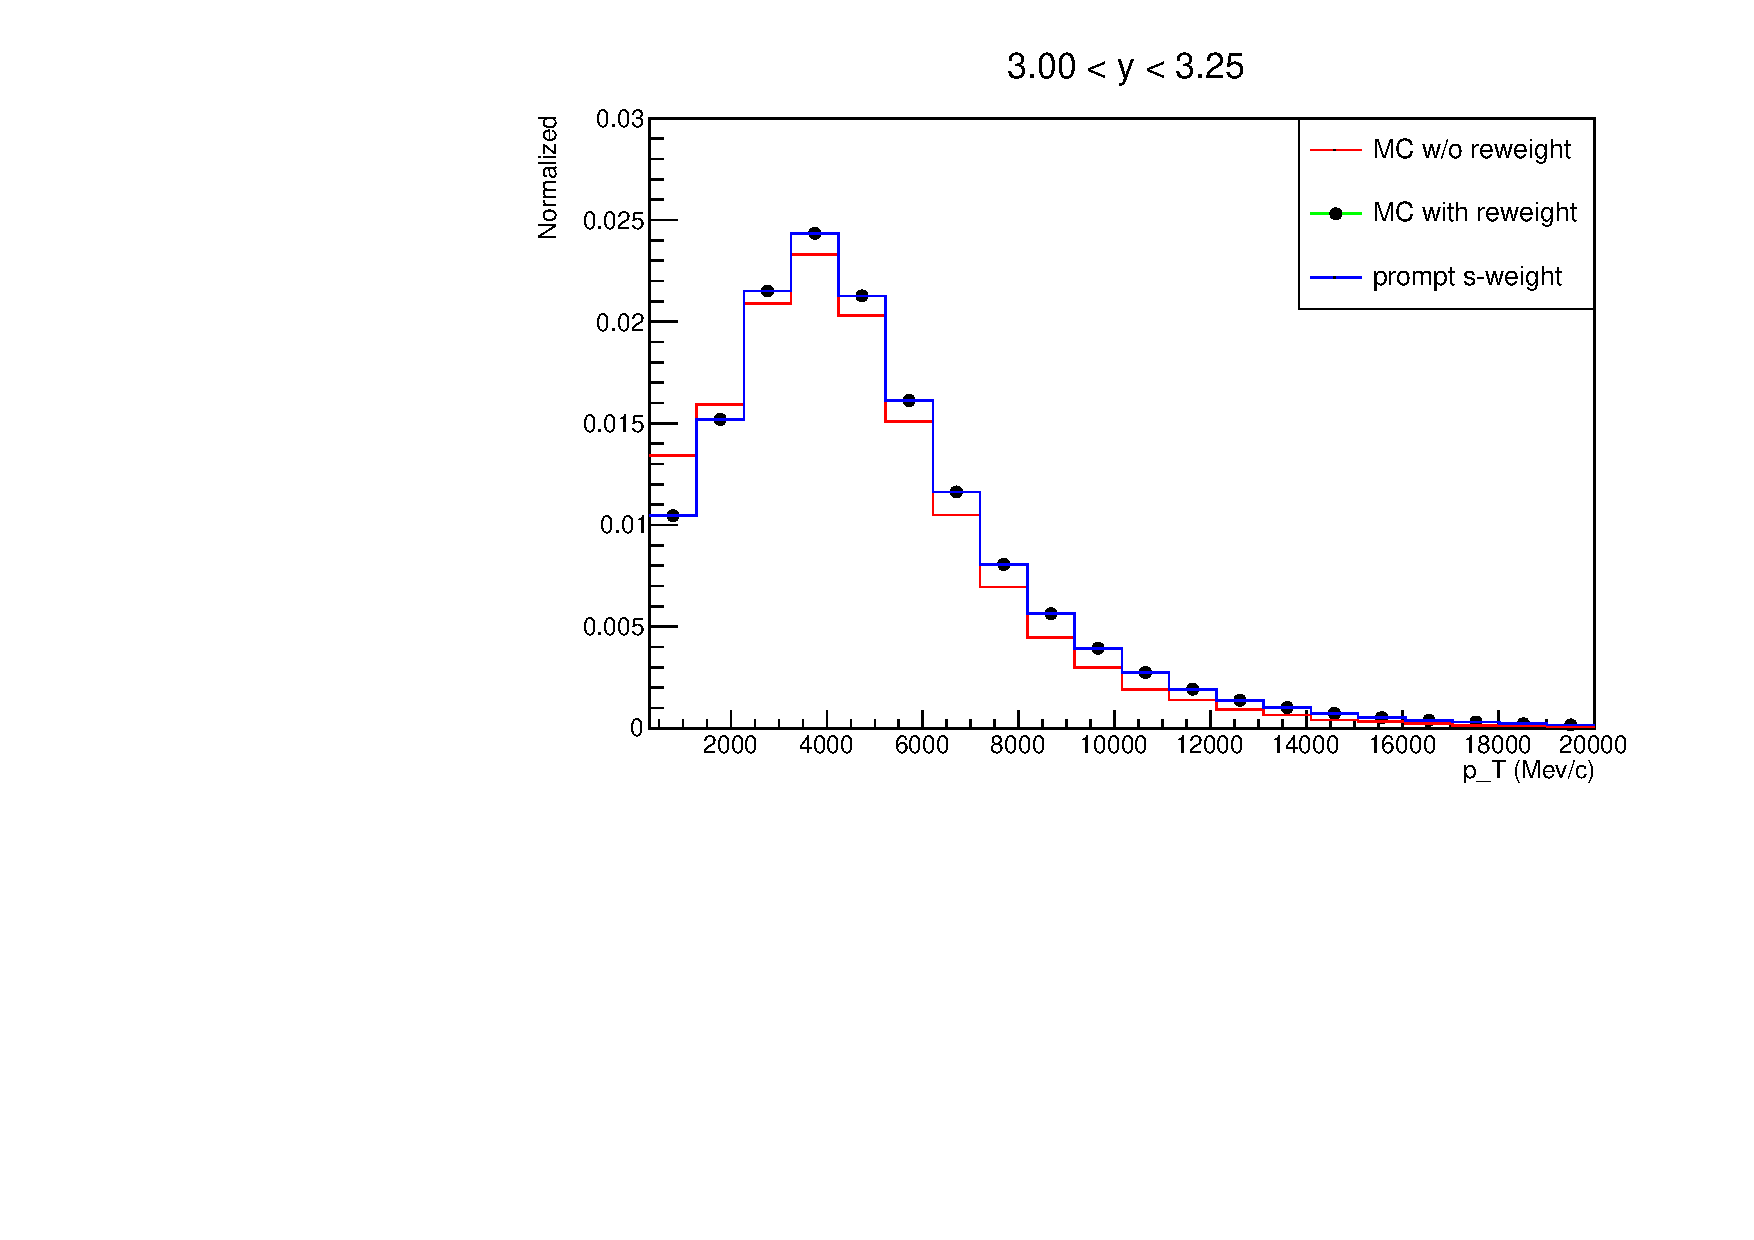
\includegraphics[width=0.19\linewidth]{pdf/Jpsi/reweight/Yb5.pdf}
      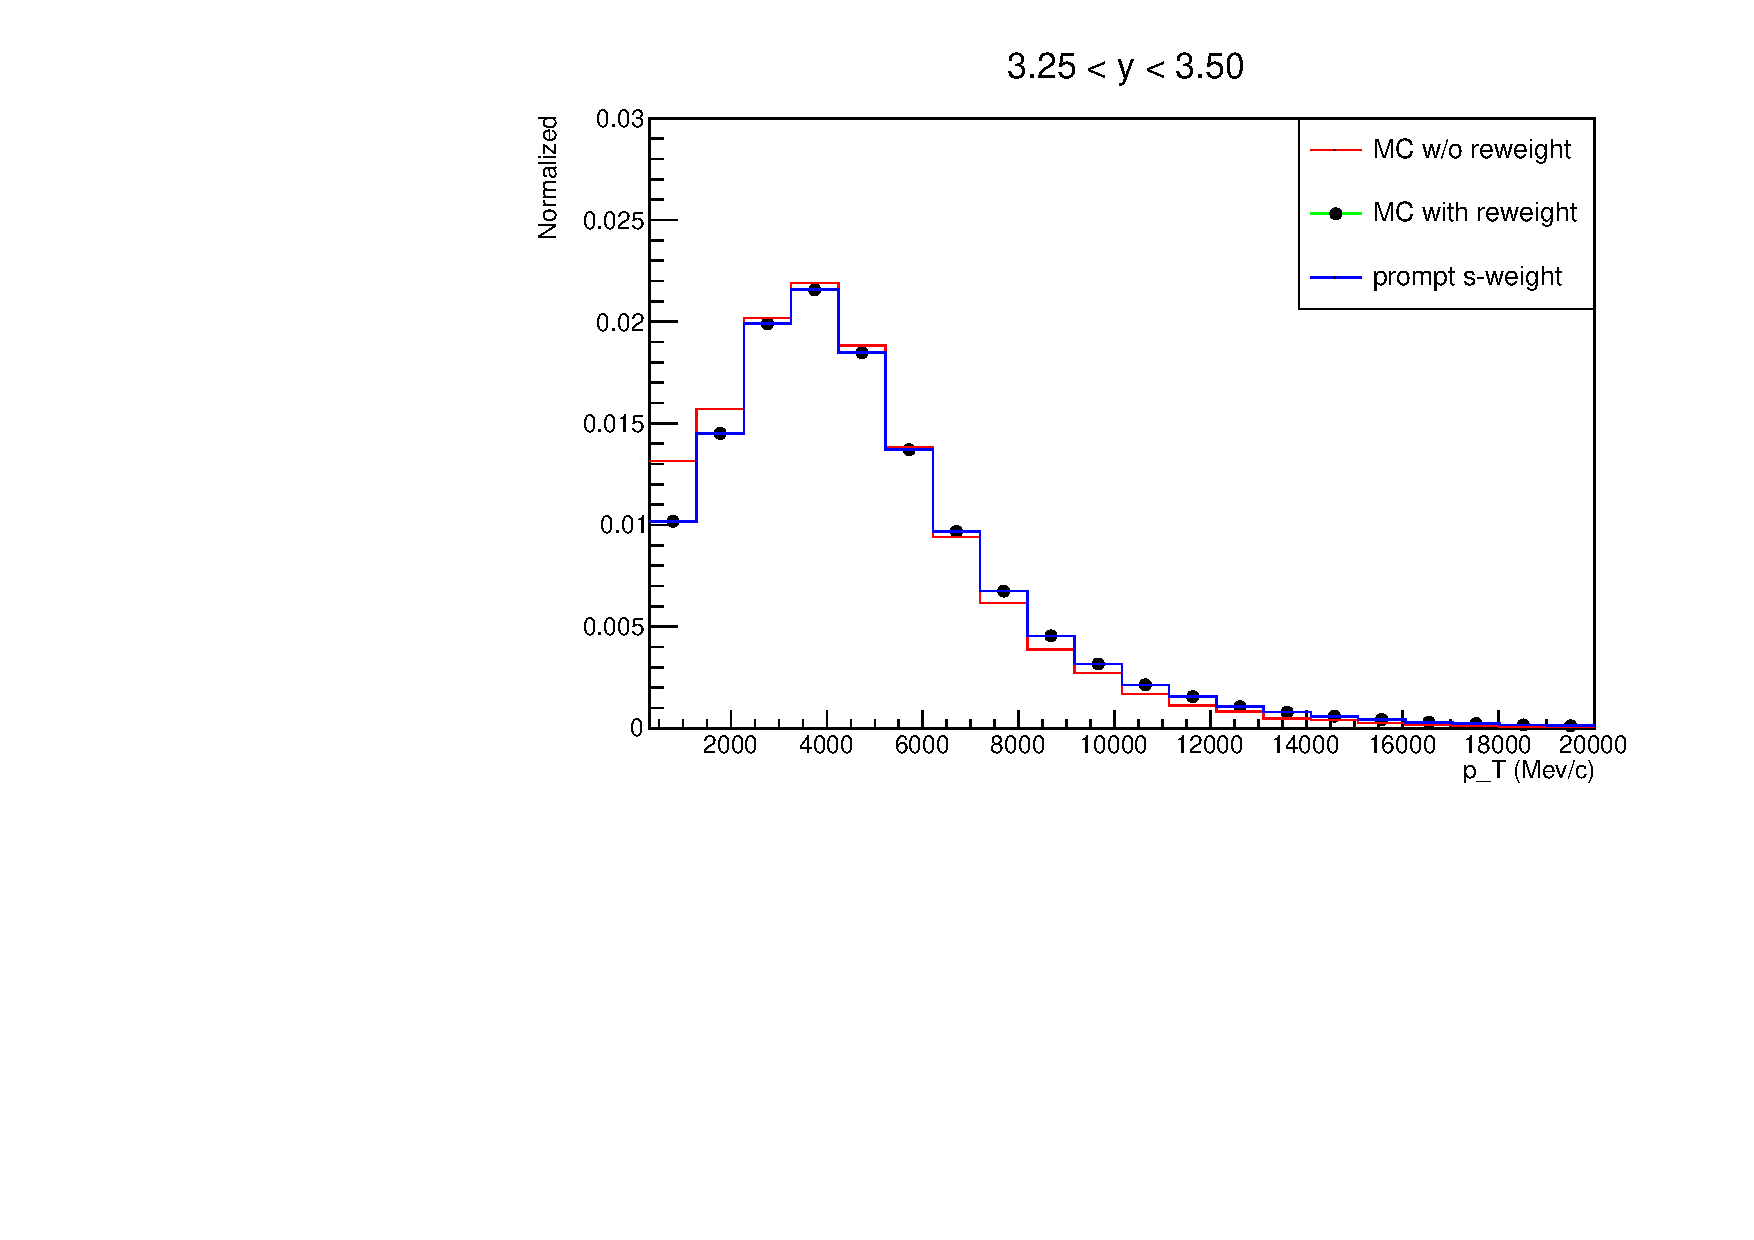
\includegraphics[width=0.19\linewidth]{pdf/Jpsi/reweight/Yb6.pdf}
      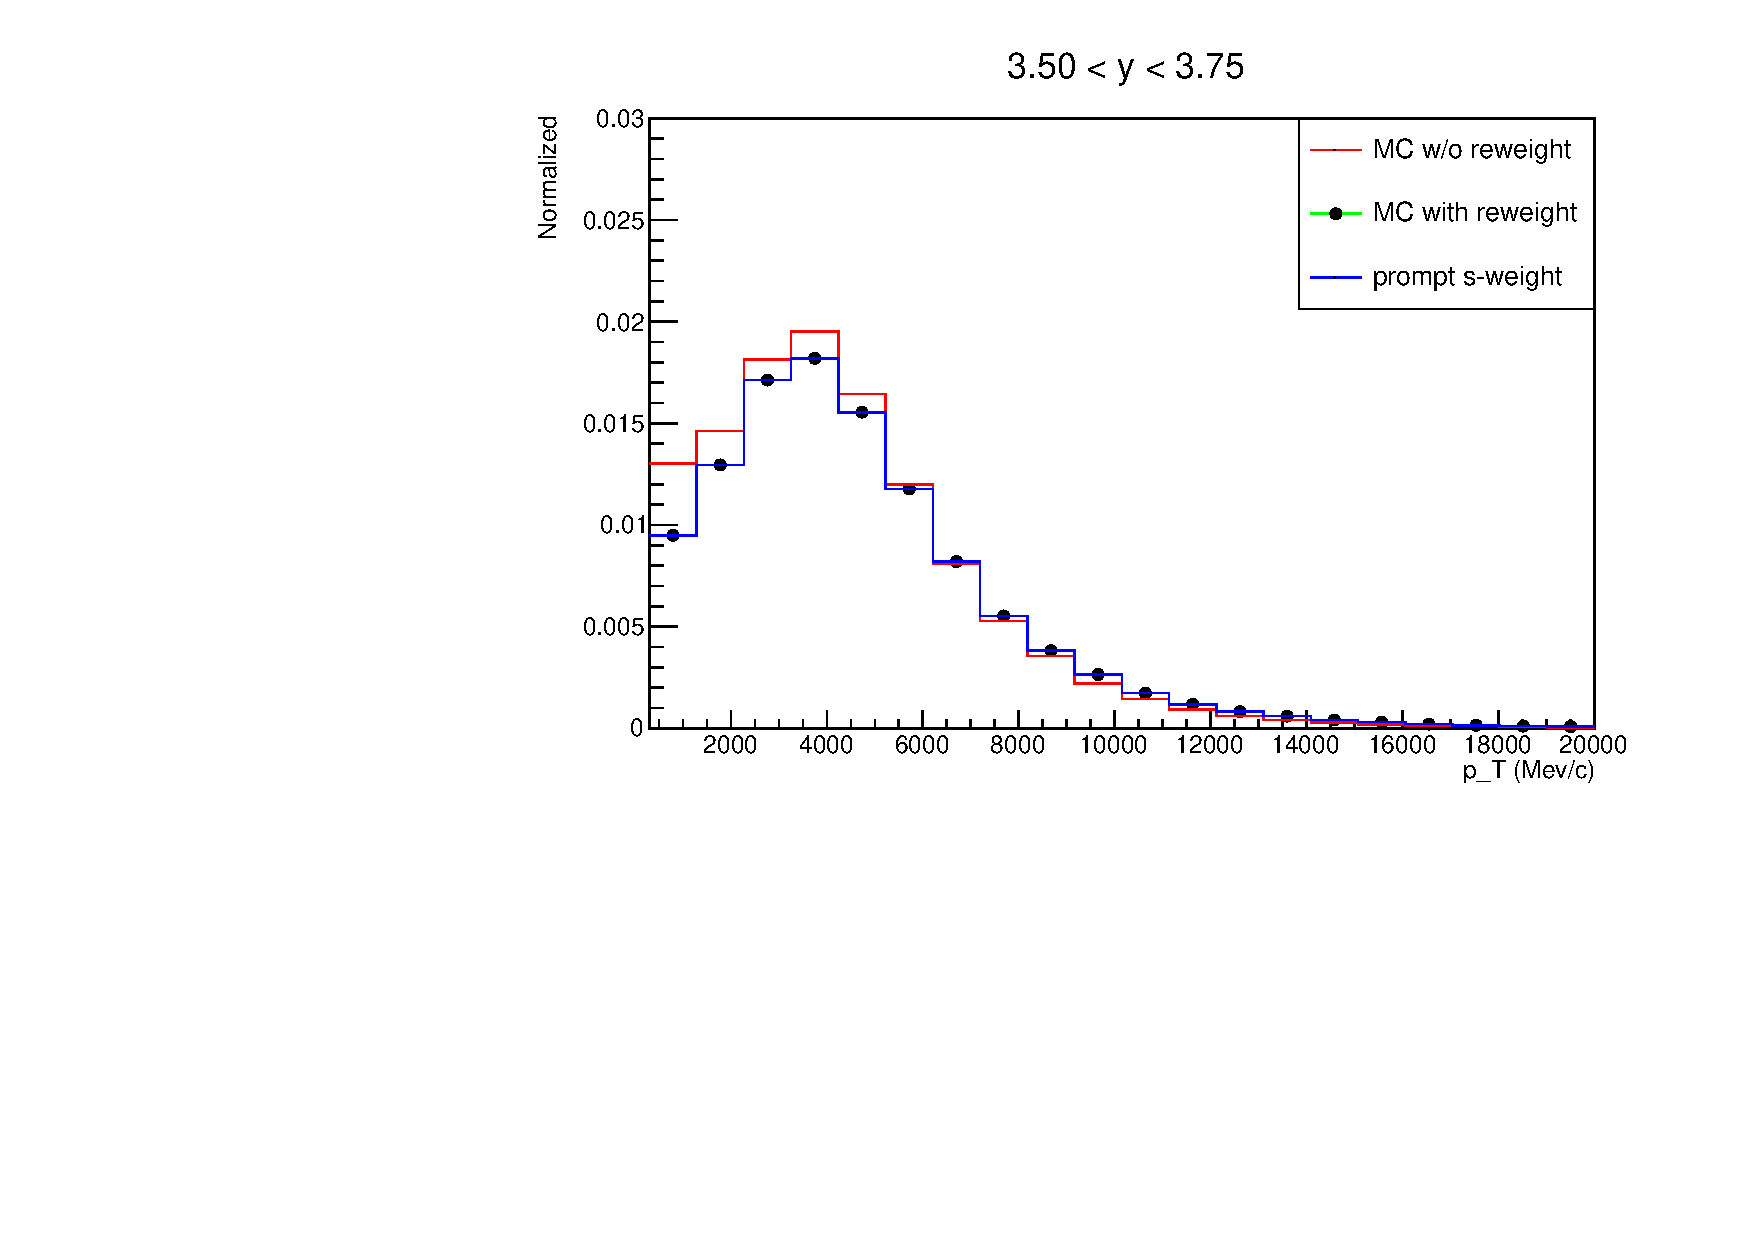
\includegraphics[width=0.19\linewidth]{pdf/Jpsi/reweight/Yb7.pdf}
      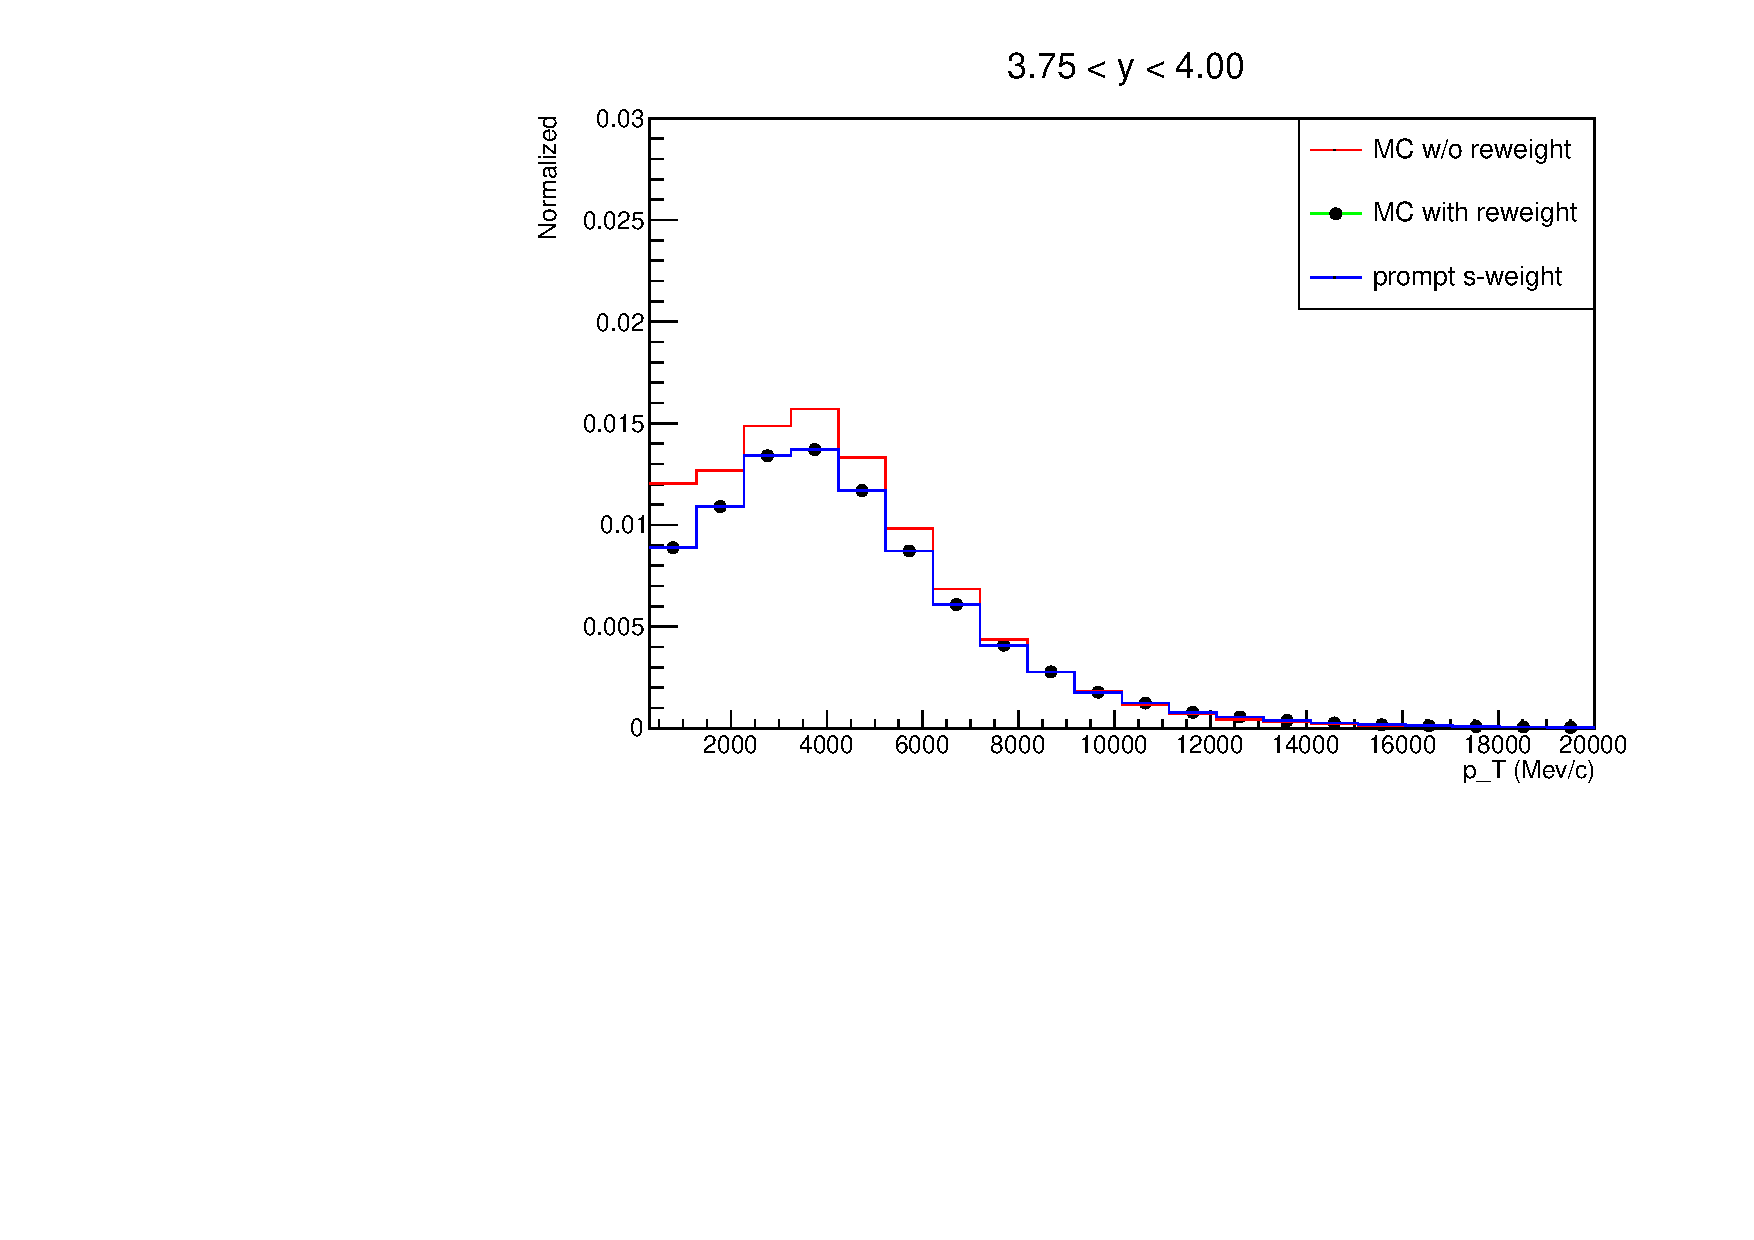
\includegraphics[width=0.19\linewidth]{pdf/Jpsi/reweight/Yb8.pdf}
      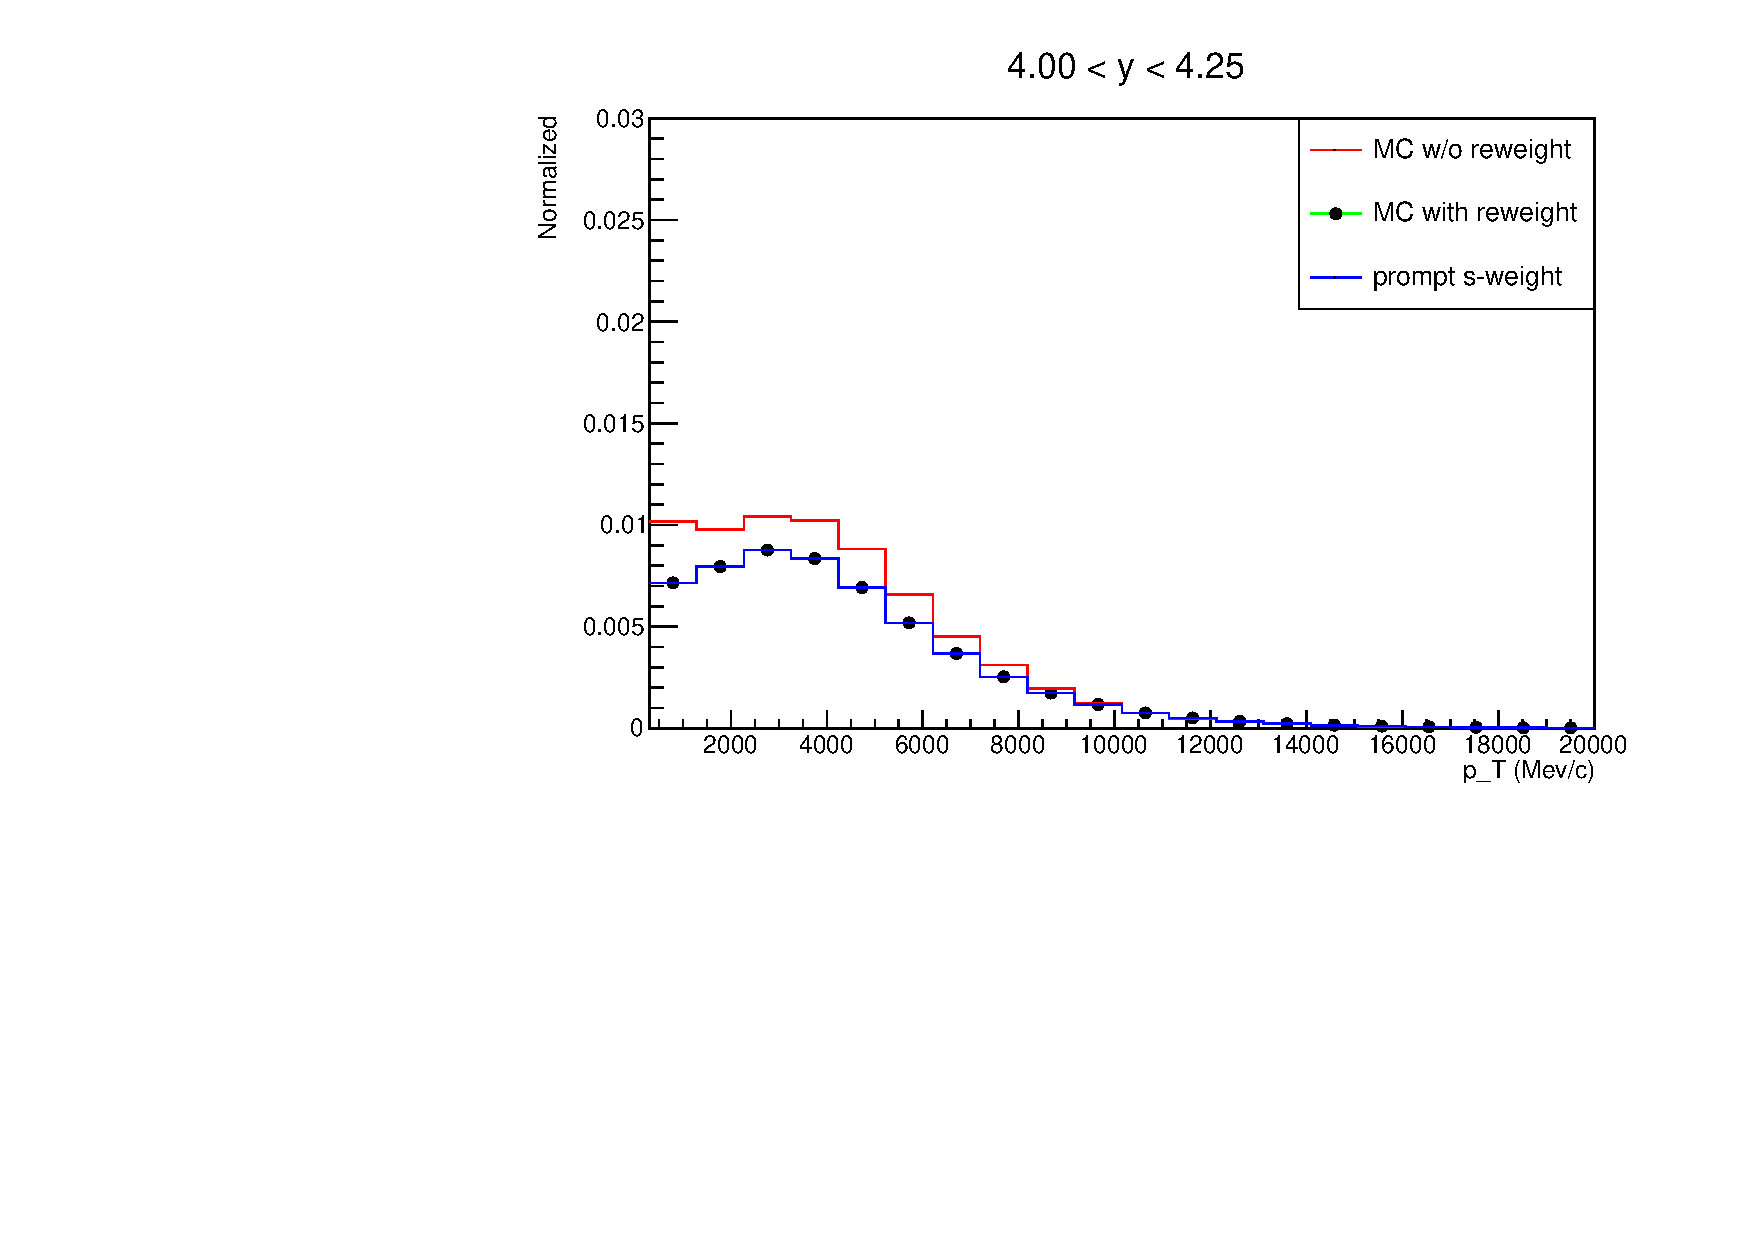
\includegraphics[width=0.19\linewidth]{pdf/Jpsi/reweight/Yb9.pdf}
      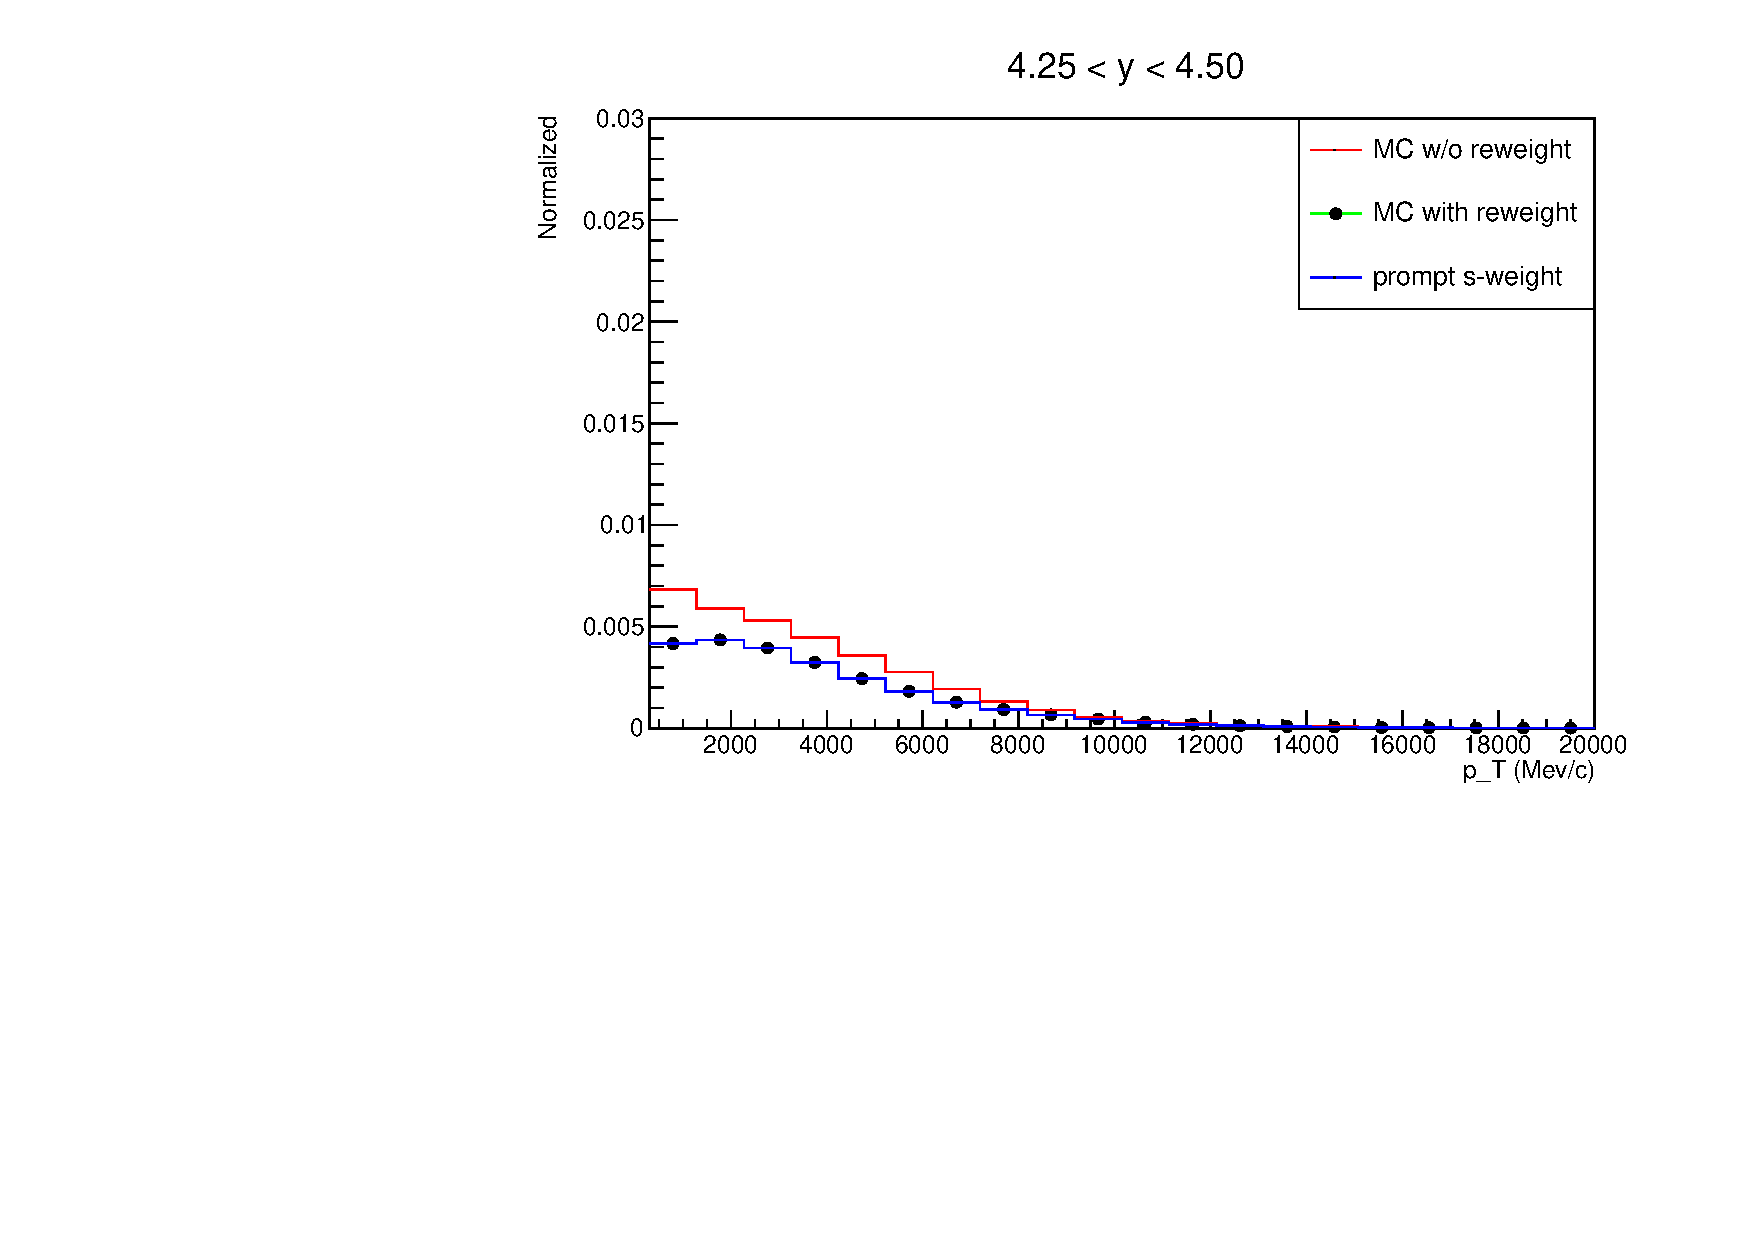
\includegraphics[width=0.19\linewidth]{pdf/Jpsi/reweight/Yb10.pdf}
    \end{center}
    \caption{
		Reweight the \pt-$y$ distribution to match MC to s-weight data. The first two rows are results of prompt \jpsi and the rest two rows are that of non-prompt \jpsi. } 
    \label{JreweightPTY}
\end{figure}
\begin{figure}[h]
    \begin{center}
      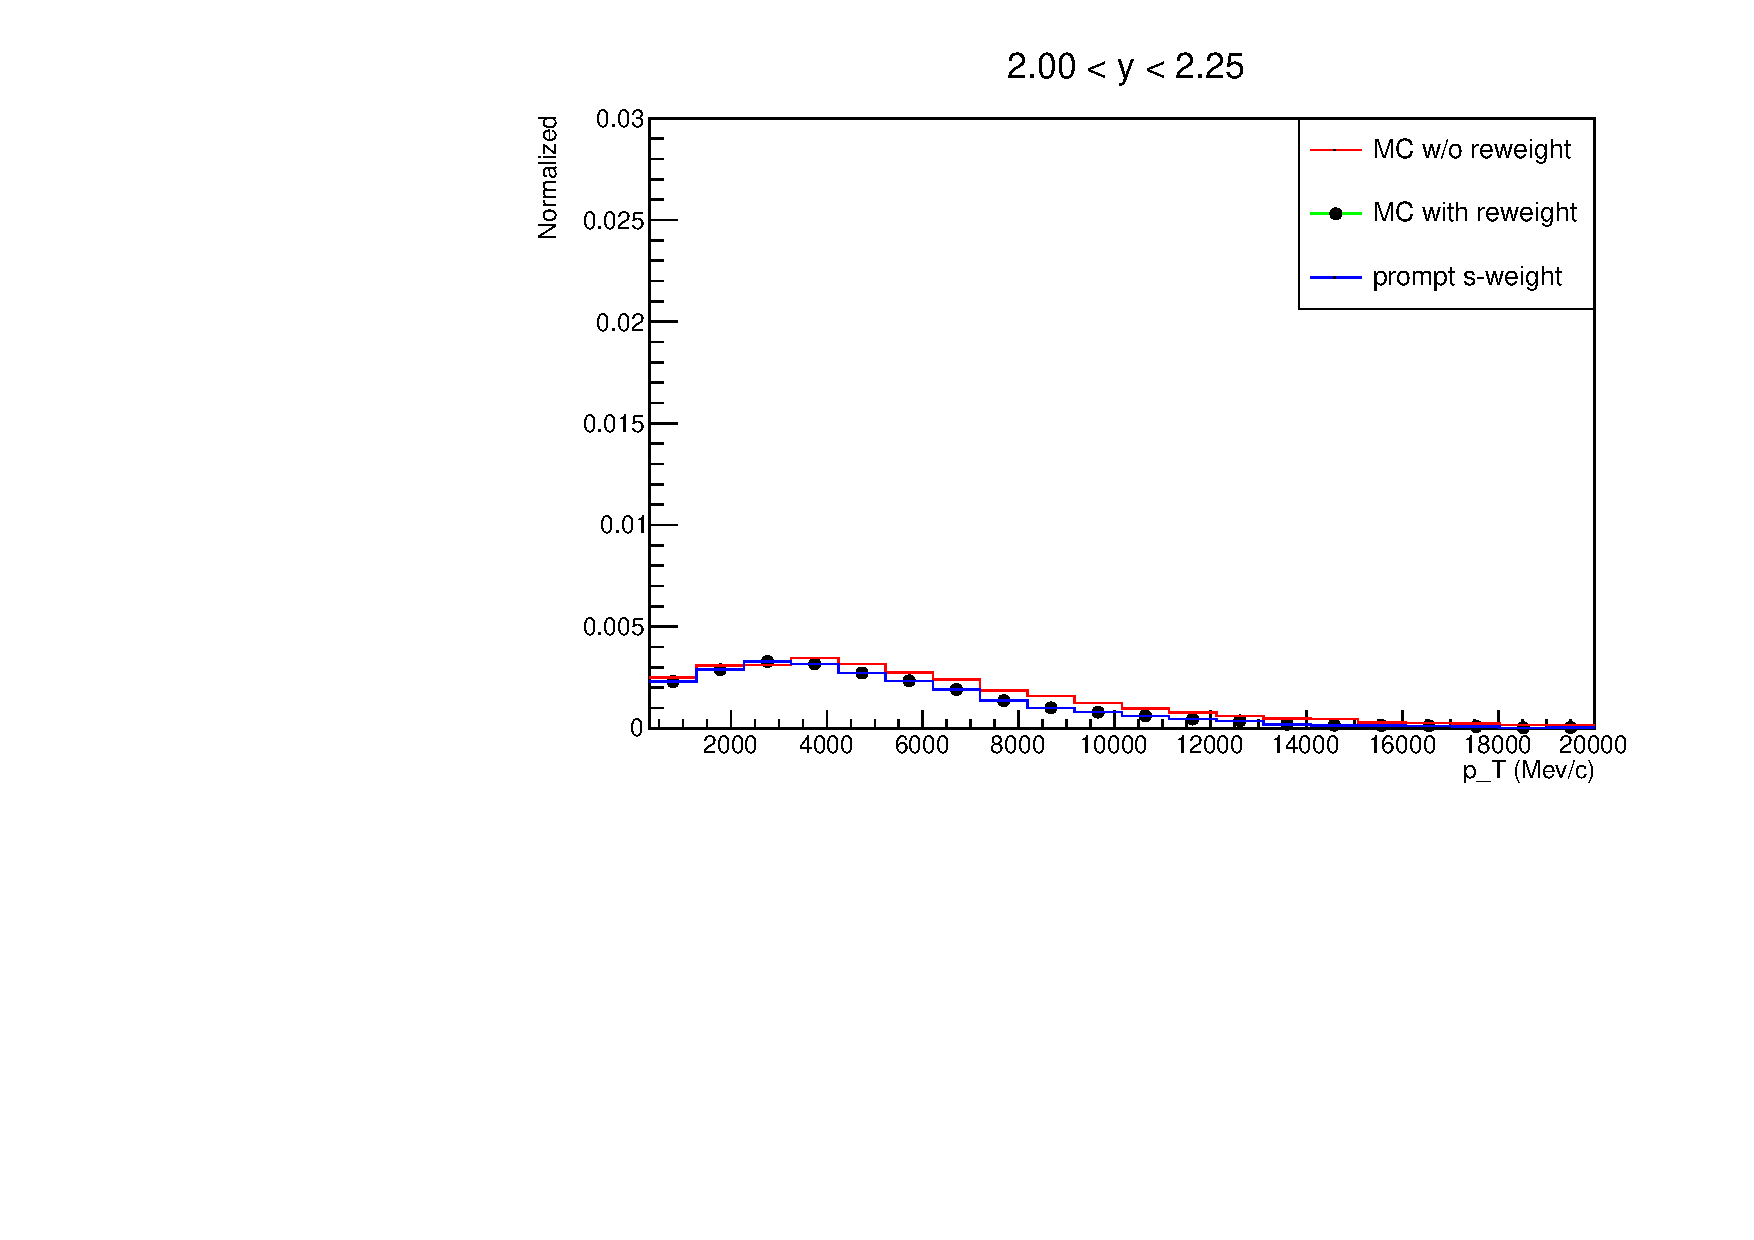
\includegraphics[width=0.19\linewidth]{pdf/Psi2S/reweight/Yp1.pdf}
      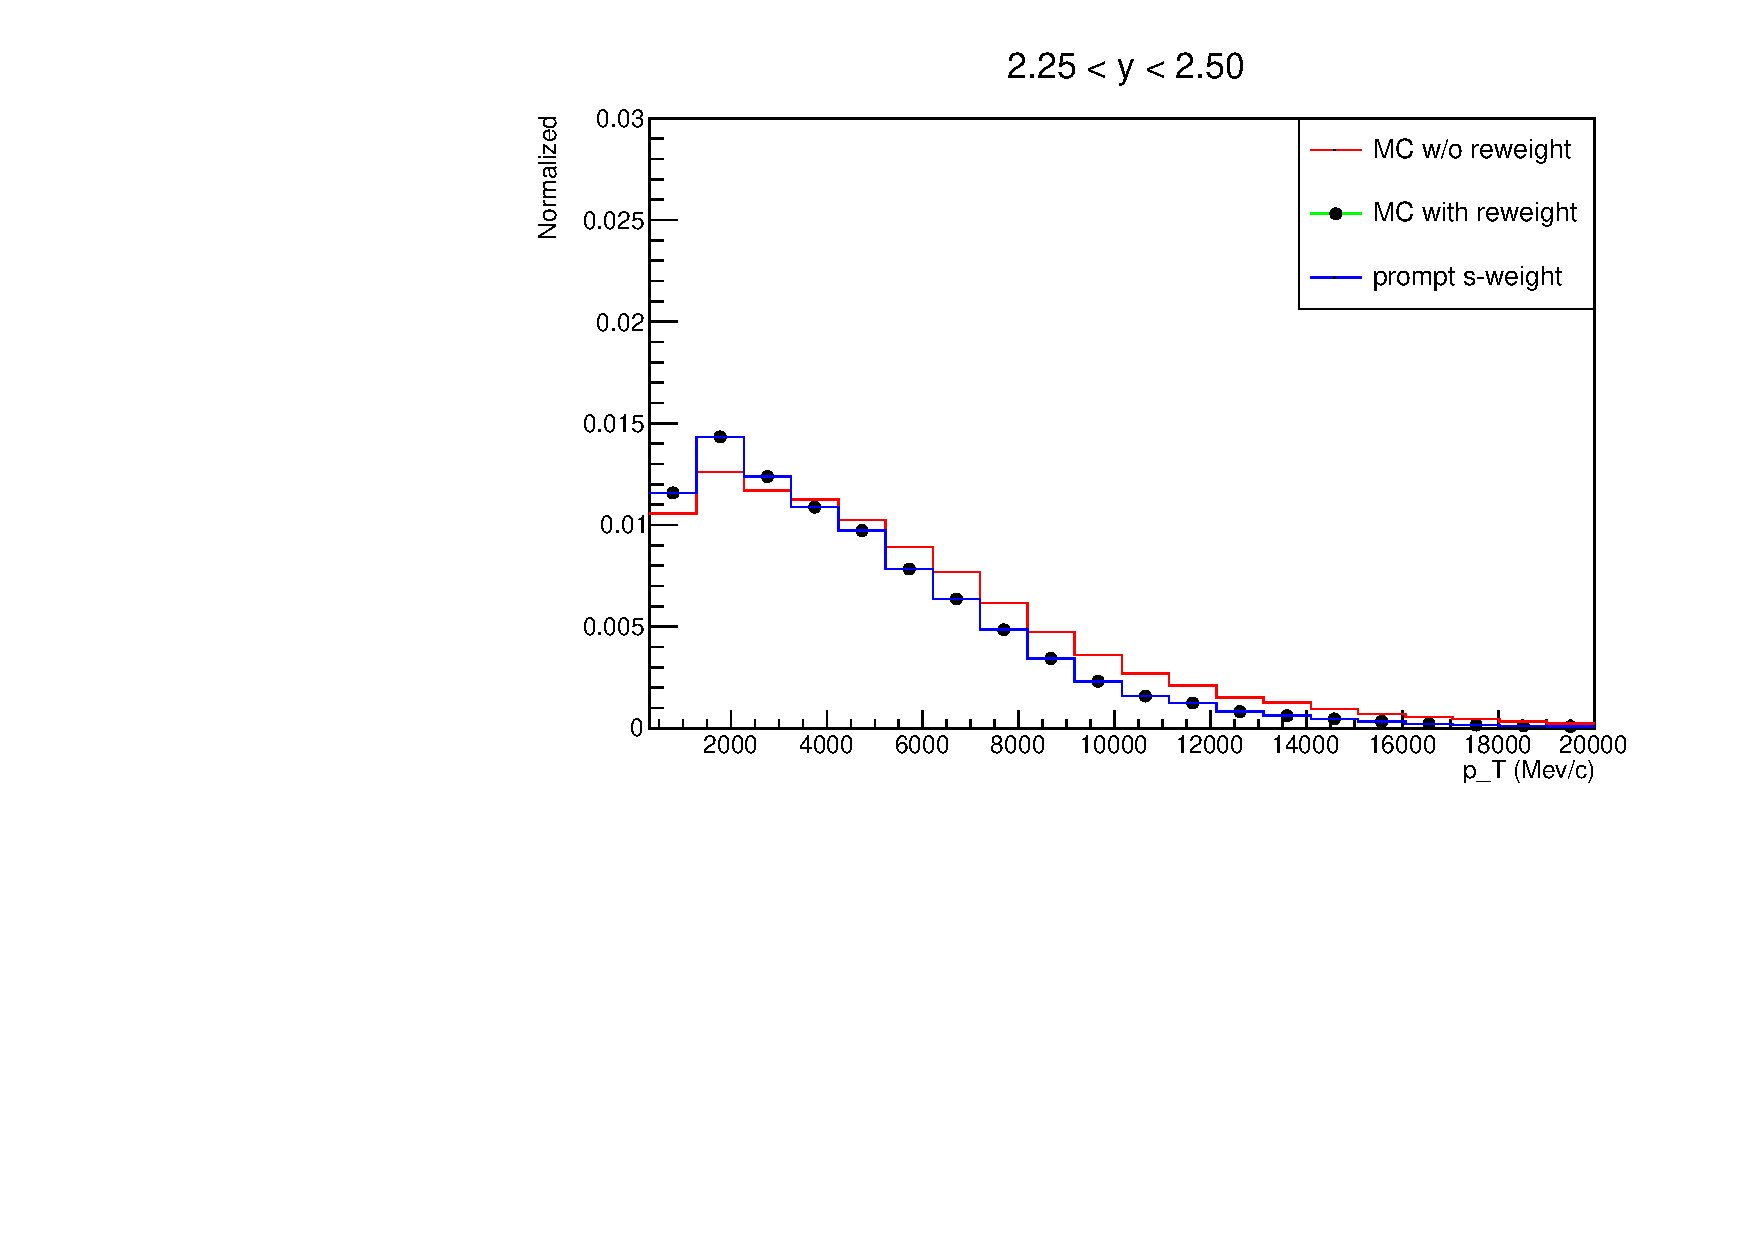
\includegraphics[width=0.19\linewidth]{pdf/Psi2S/reweight/Yp2.pdf}
      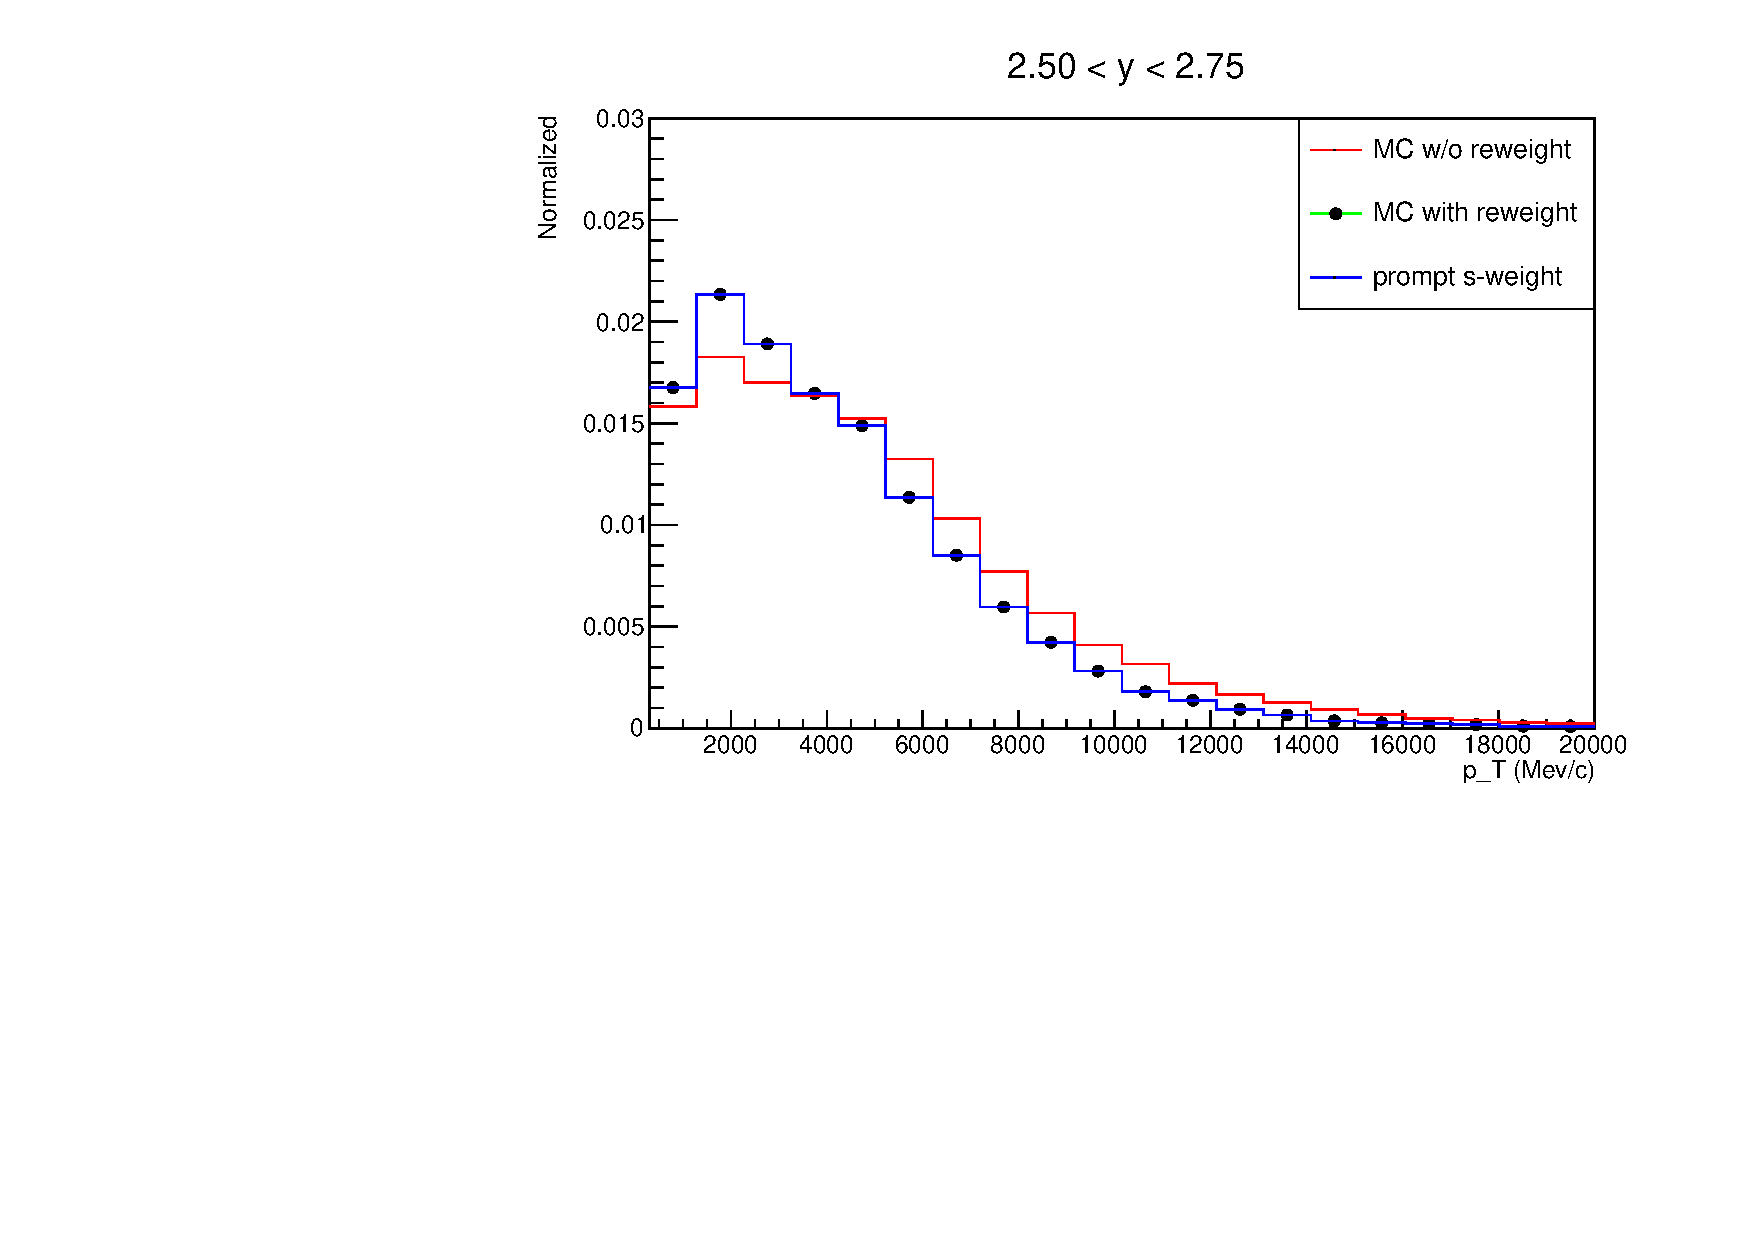
\includegraphics[width=0.19\linewidth]{pdf/Psi2S/reweight/Yp3.pdf}
      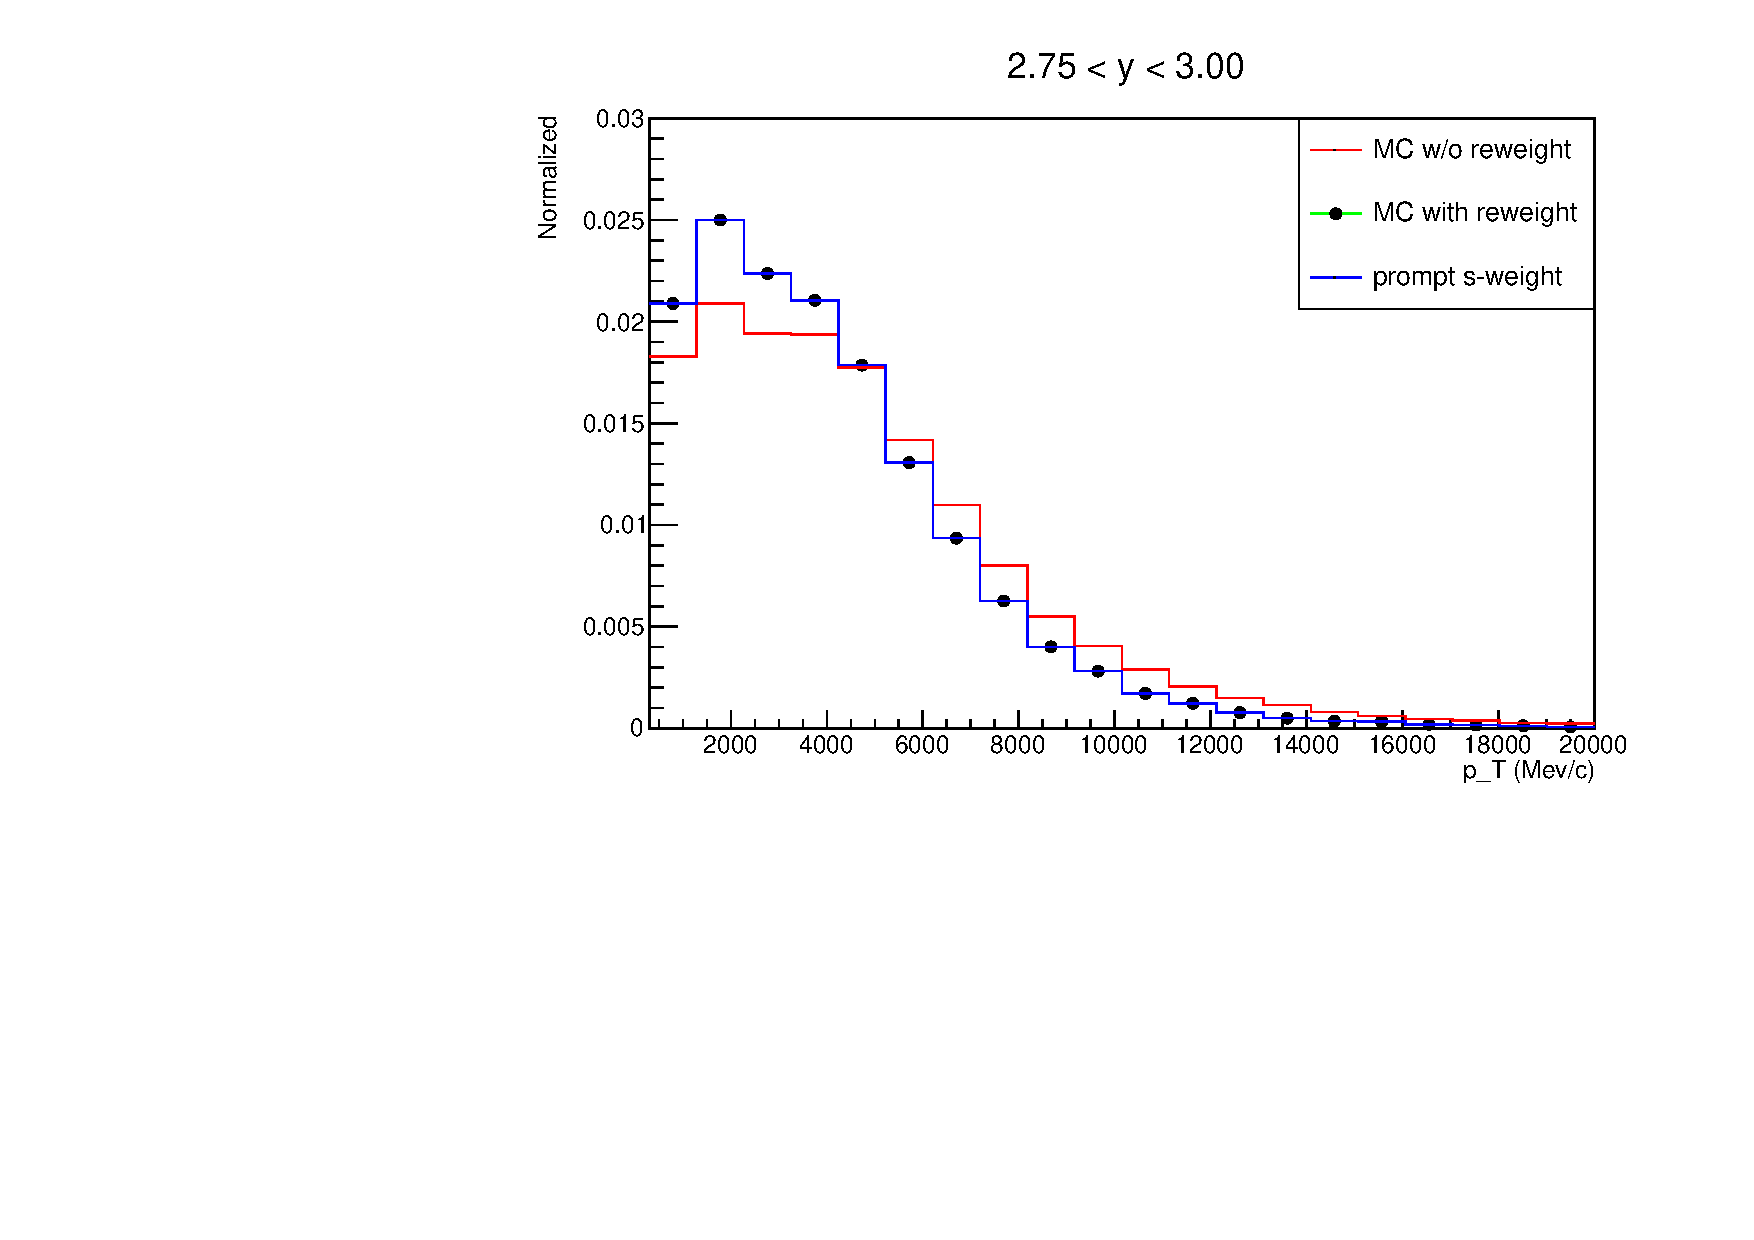
\includegraphics[width=0.19\linewidth]{pdf/Psi2S/reweight/Yp4.pdf}
      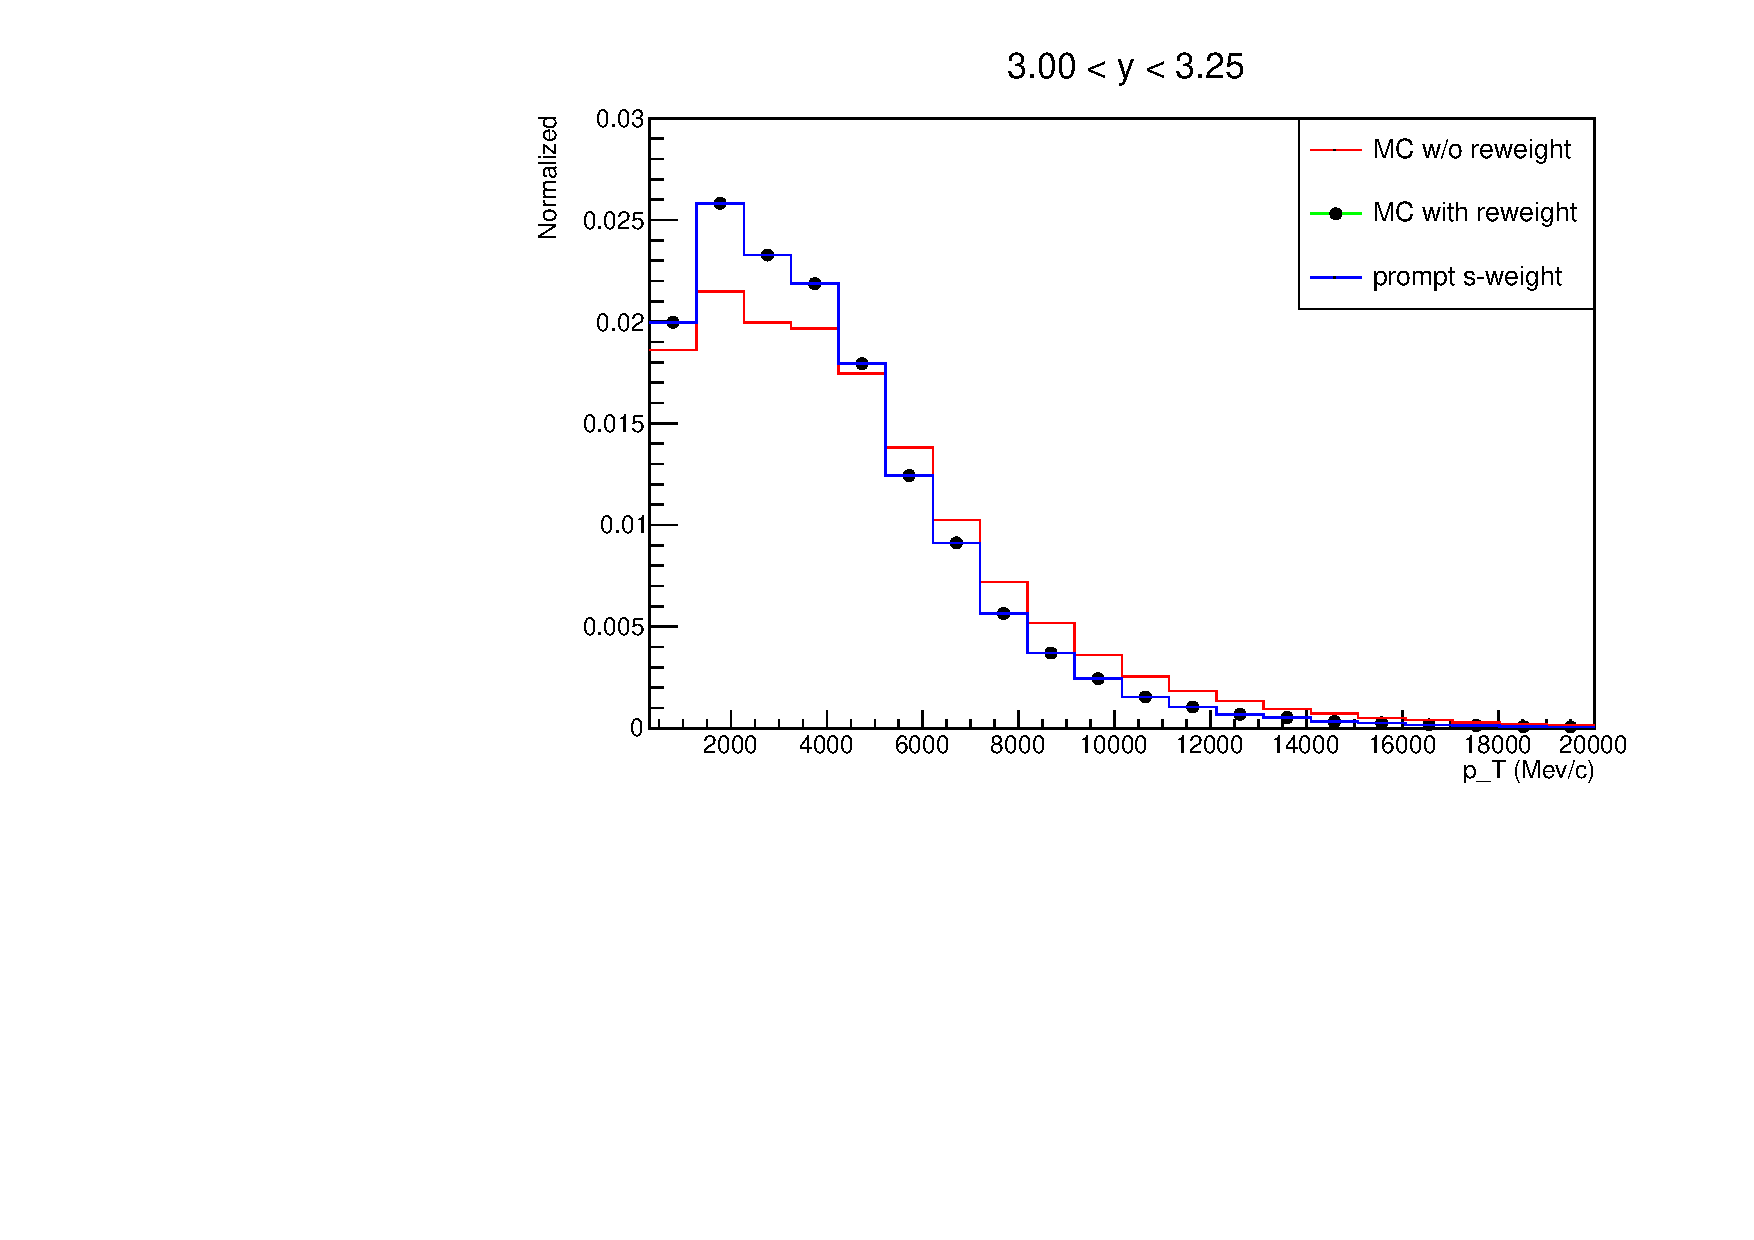
\includegraphics[width=0.19\linewidth]{pdf/Psi2S/reweight/Yp5.pdf}
      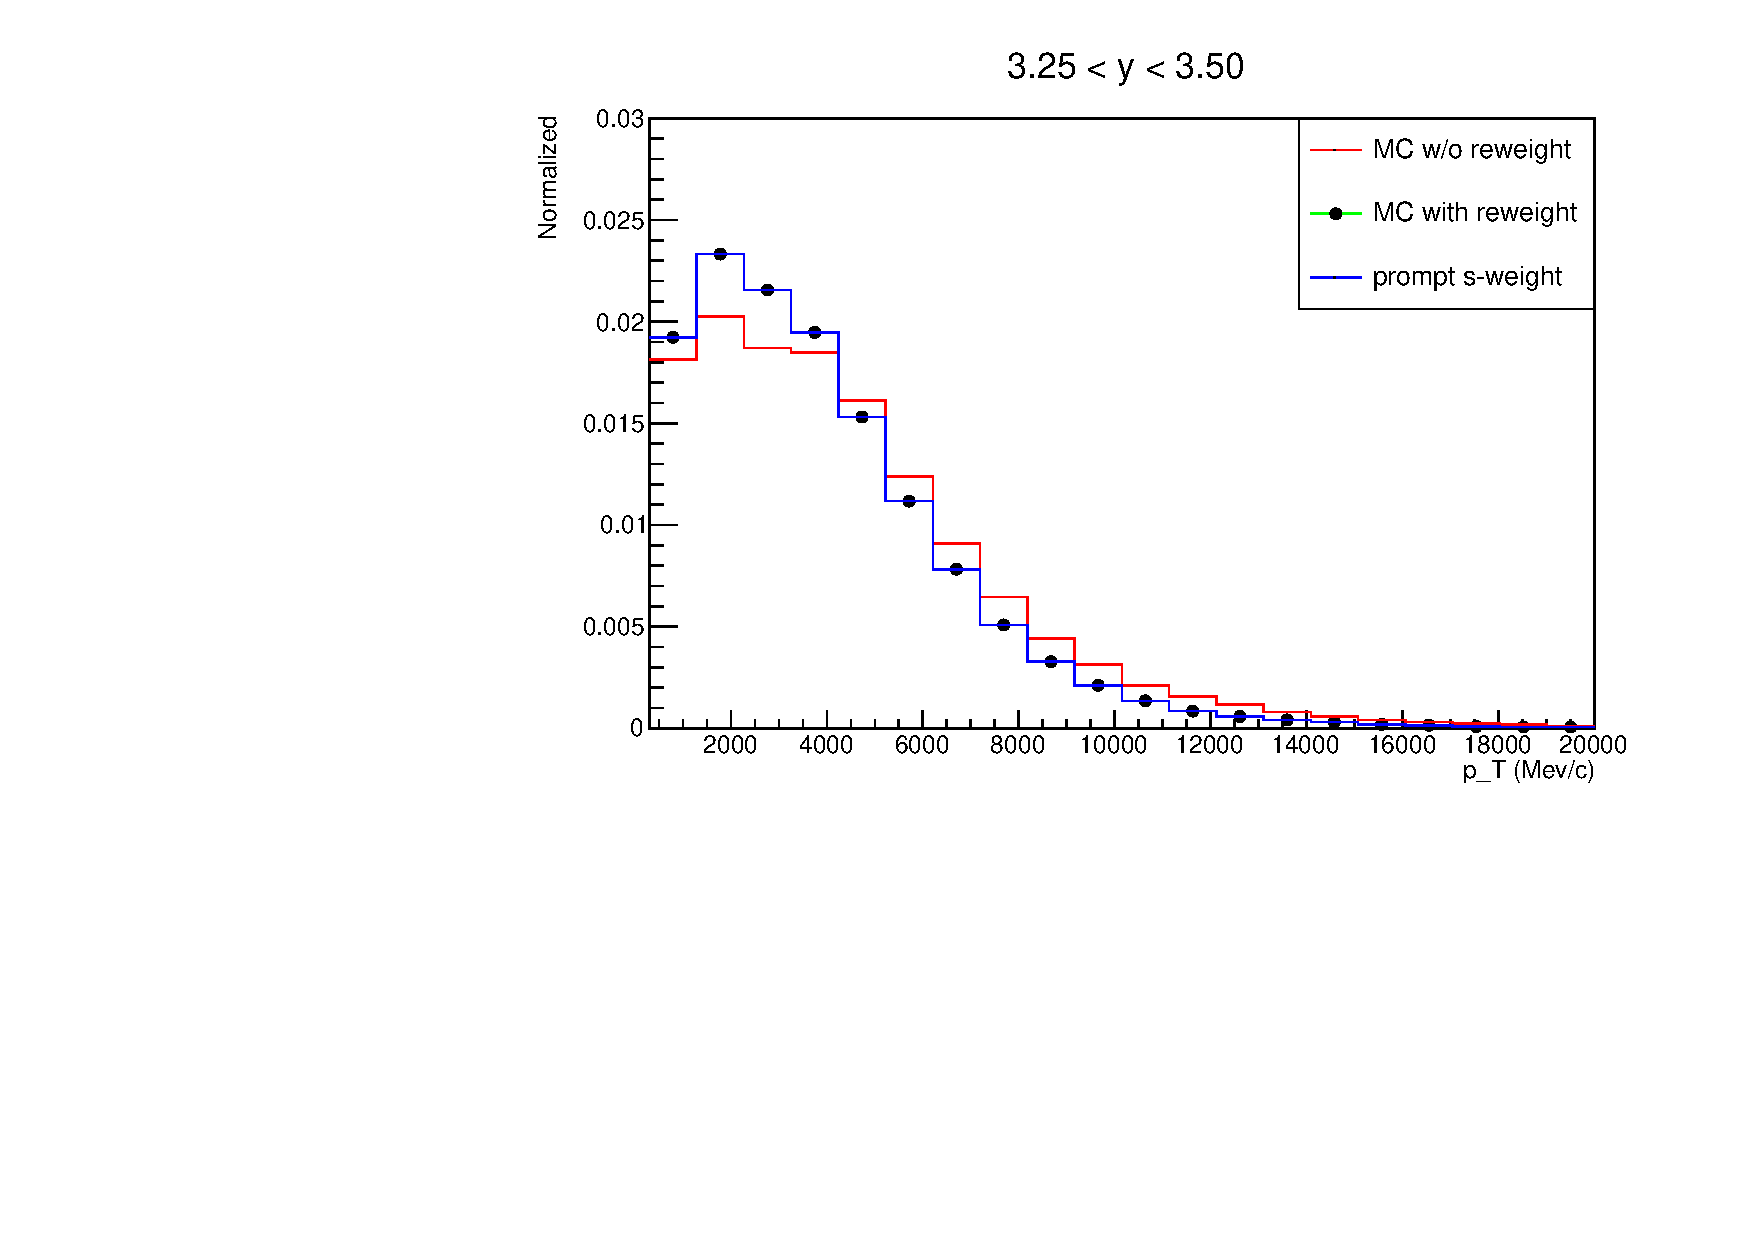
\includegraphics[width=0.19\linewidth]{pdf/Psi2S/reweight/Yp6.pdf}
      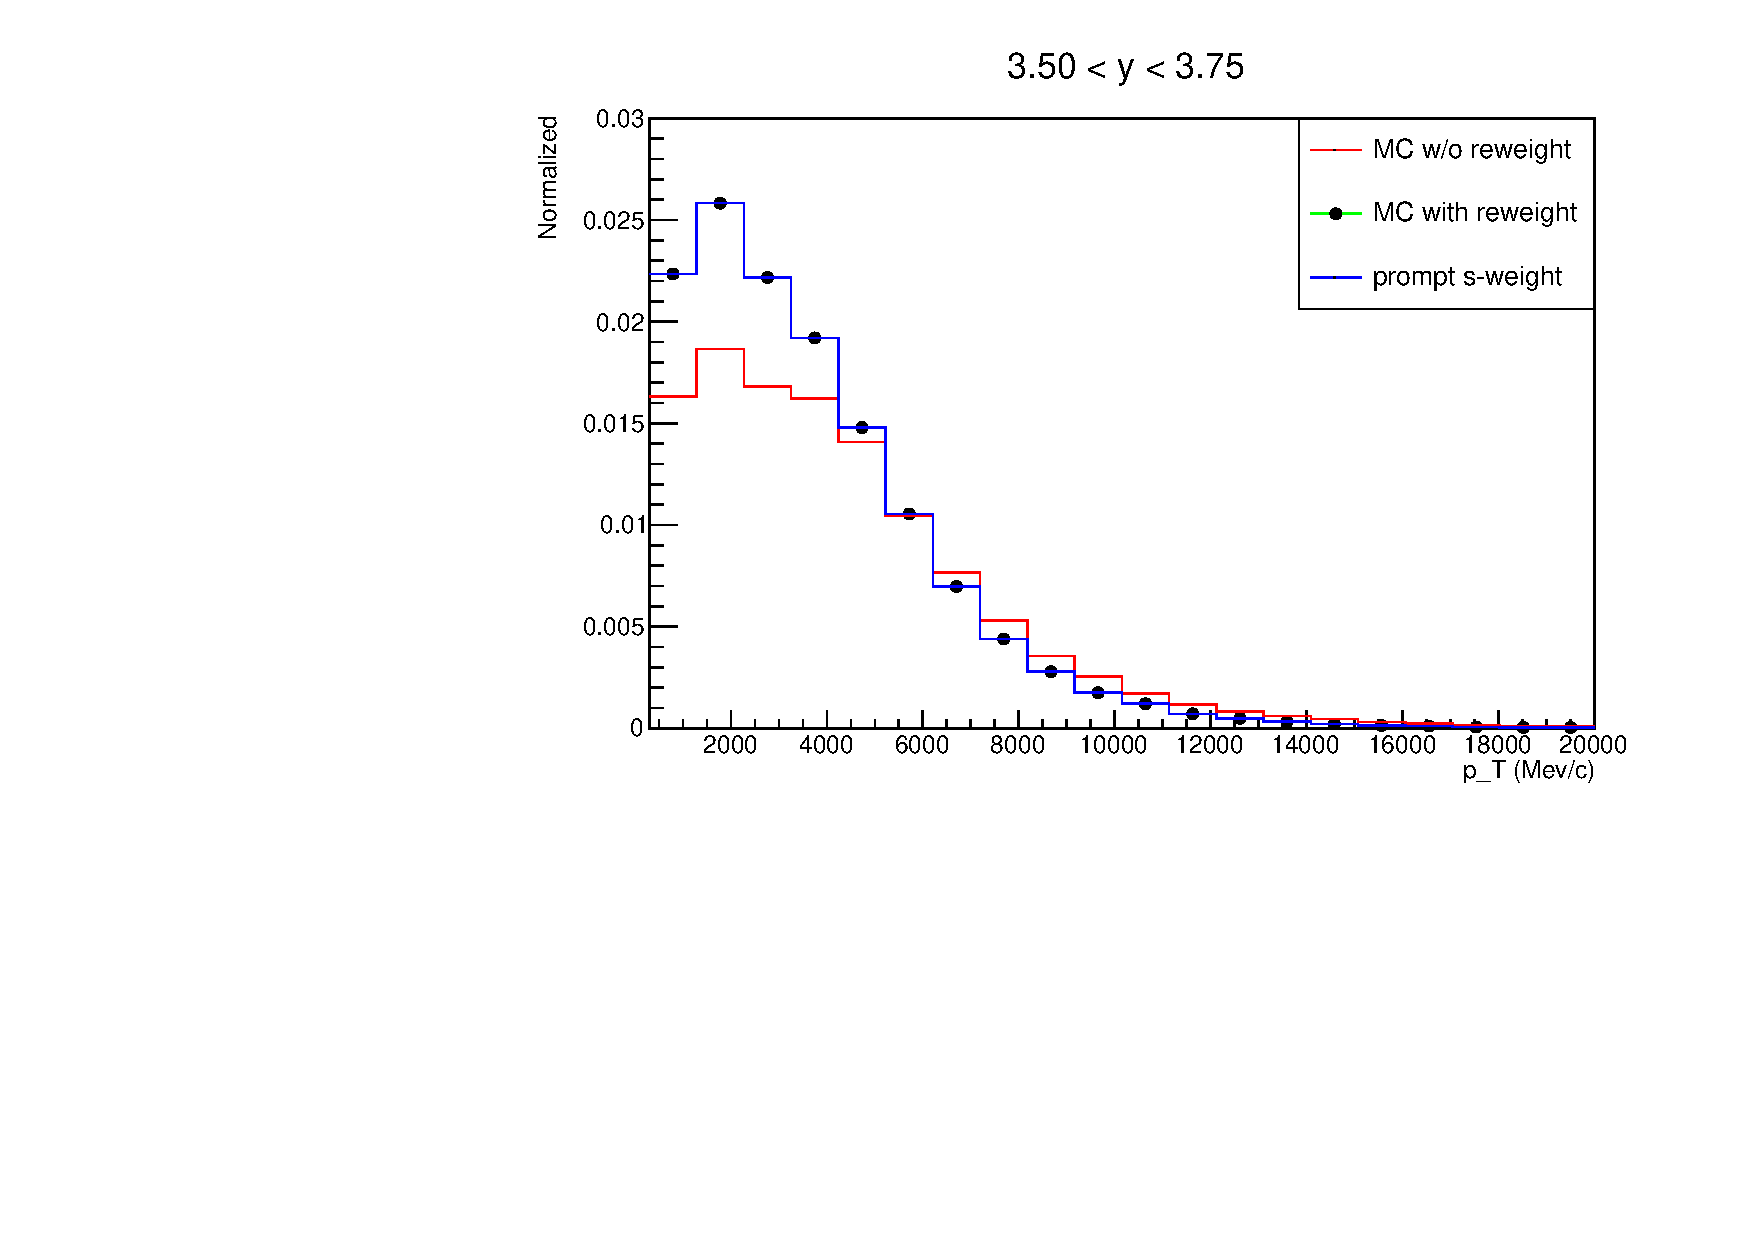
\includegraphics[width=0.19\linewidth]{pdf/Psi2S/reweight/Yp7.pdf}
      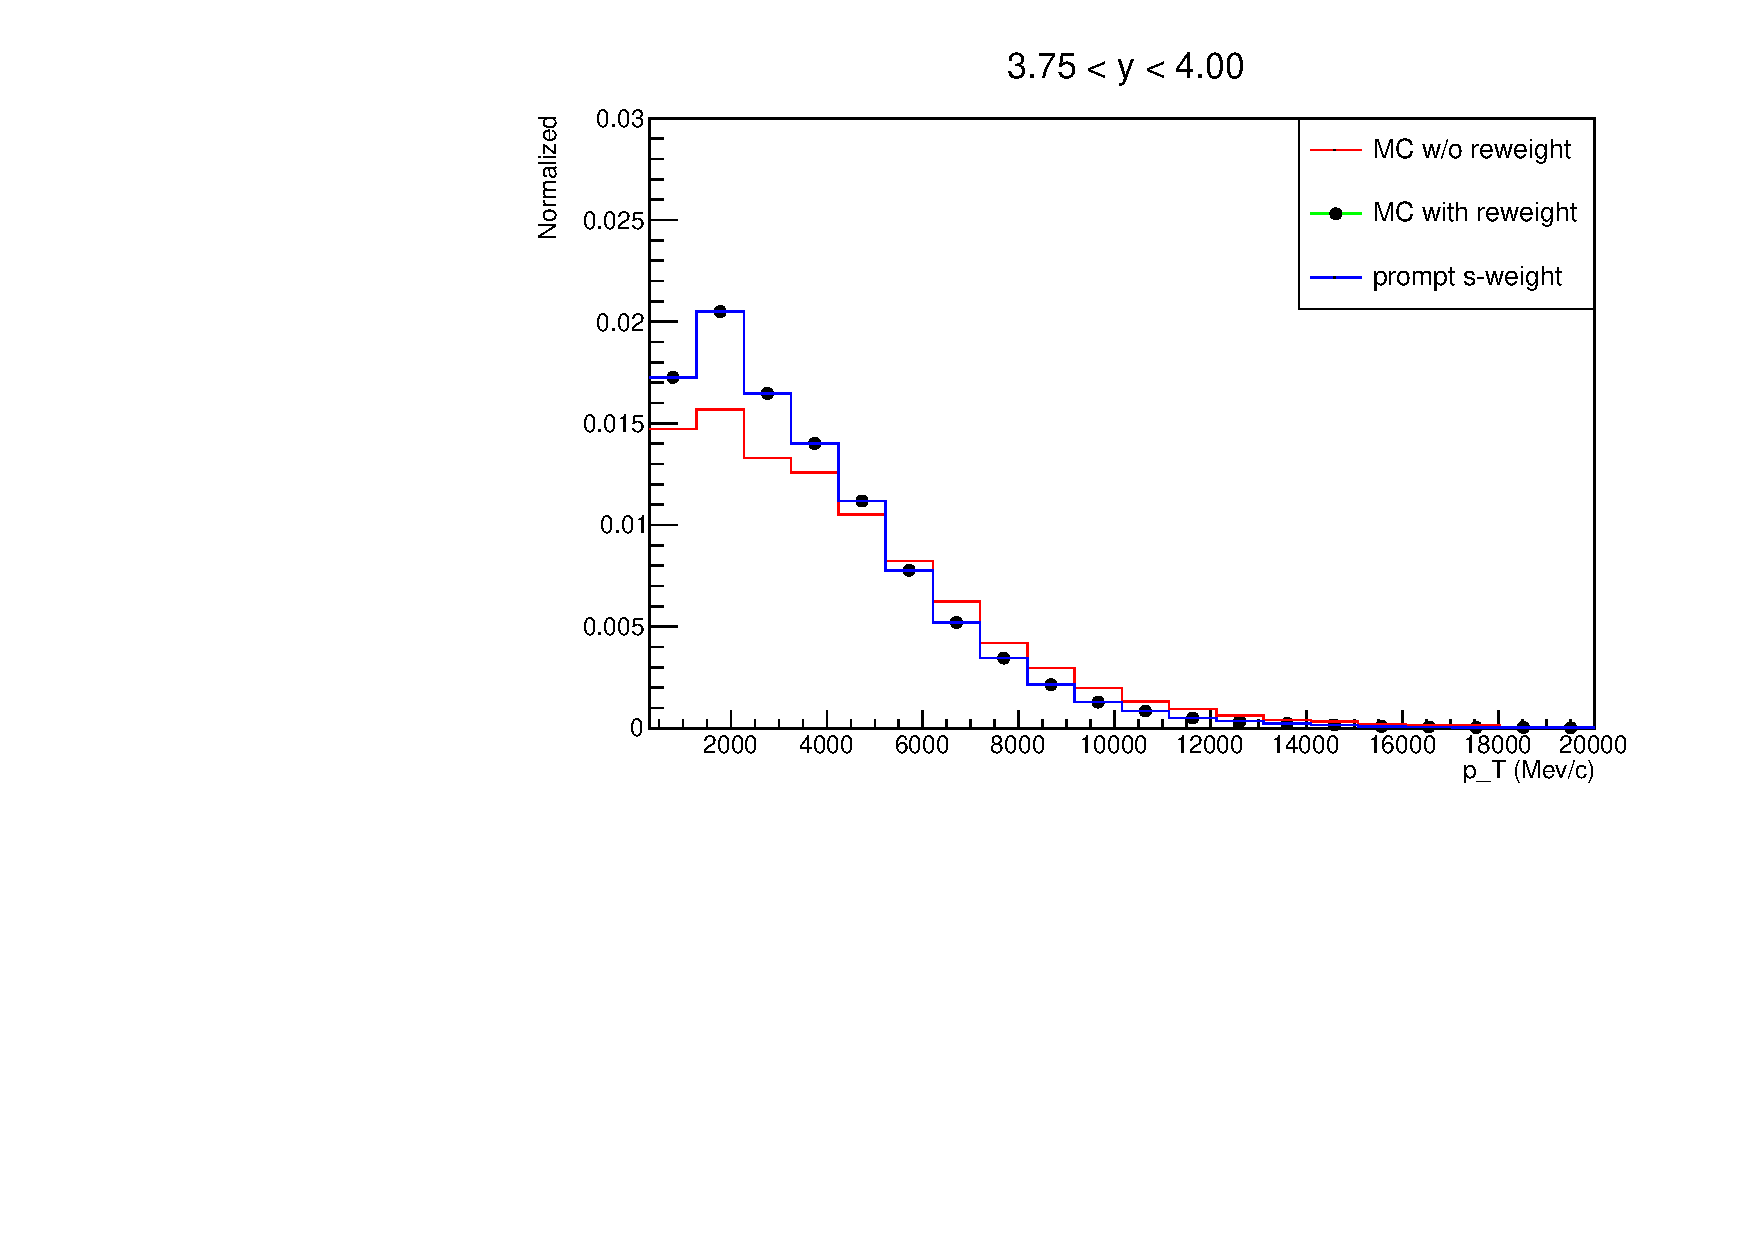
\includegraphics[width=0.19\linewidth]{pdf/Psi2S/reweight/Yp8.pdf}
      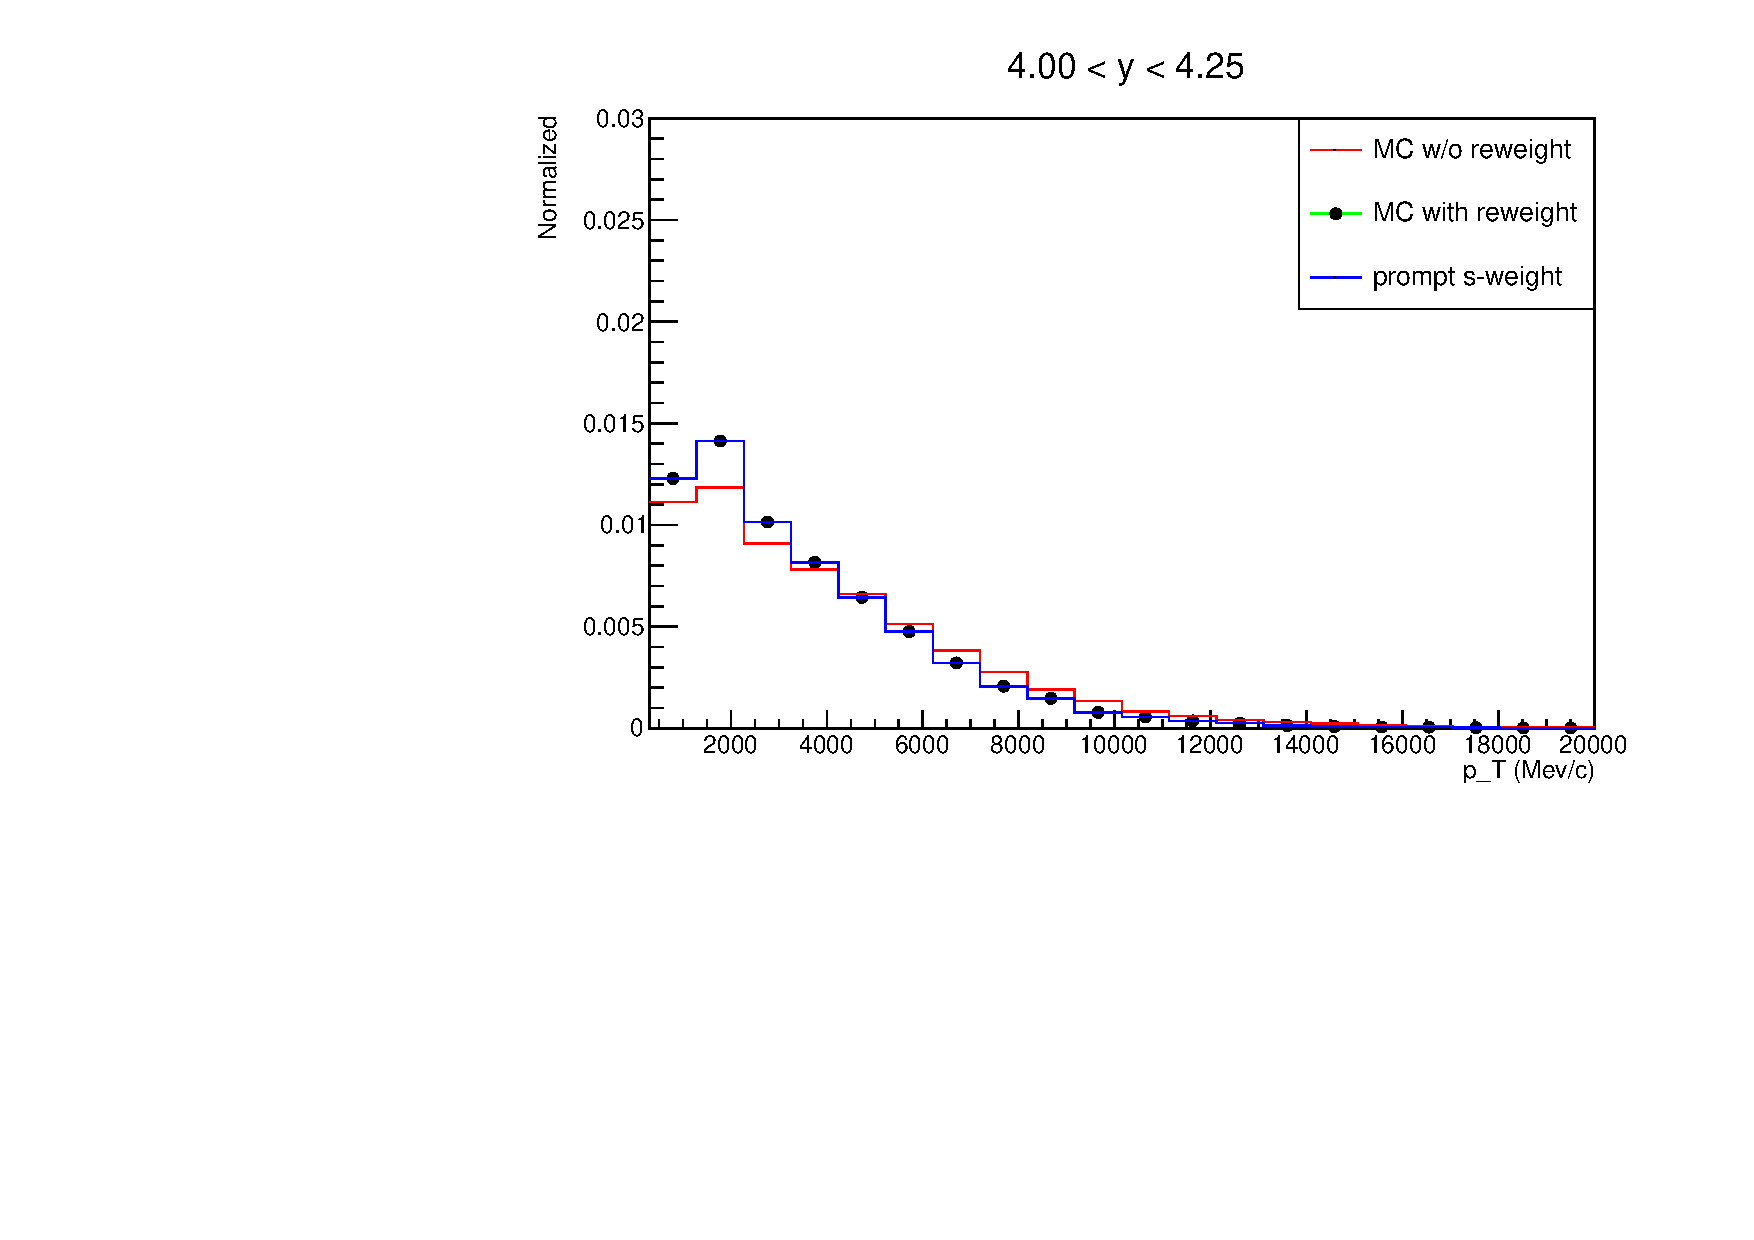
\includegraphics[width=0.19\linewidth]{pdf/Psi2S/reweight/Yp9.pdf}
      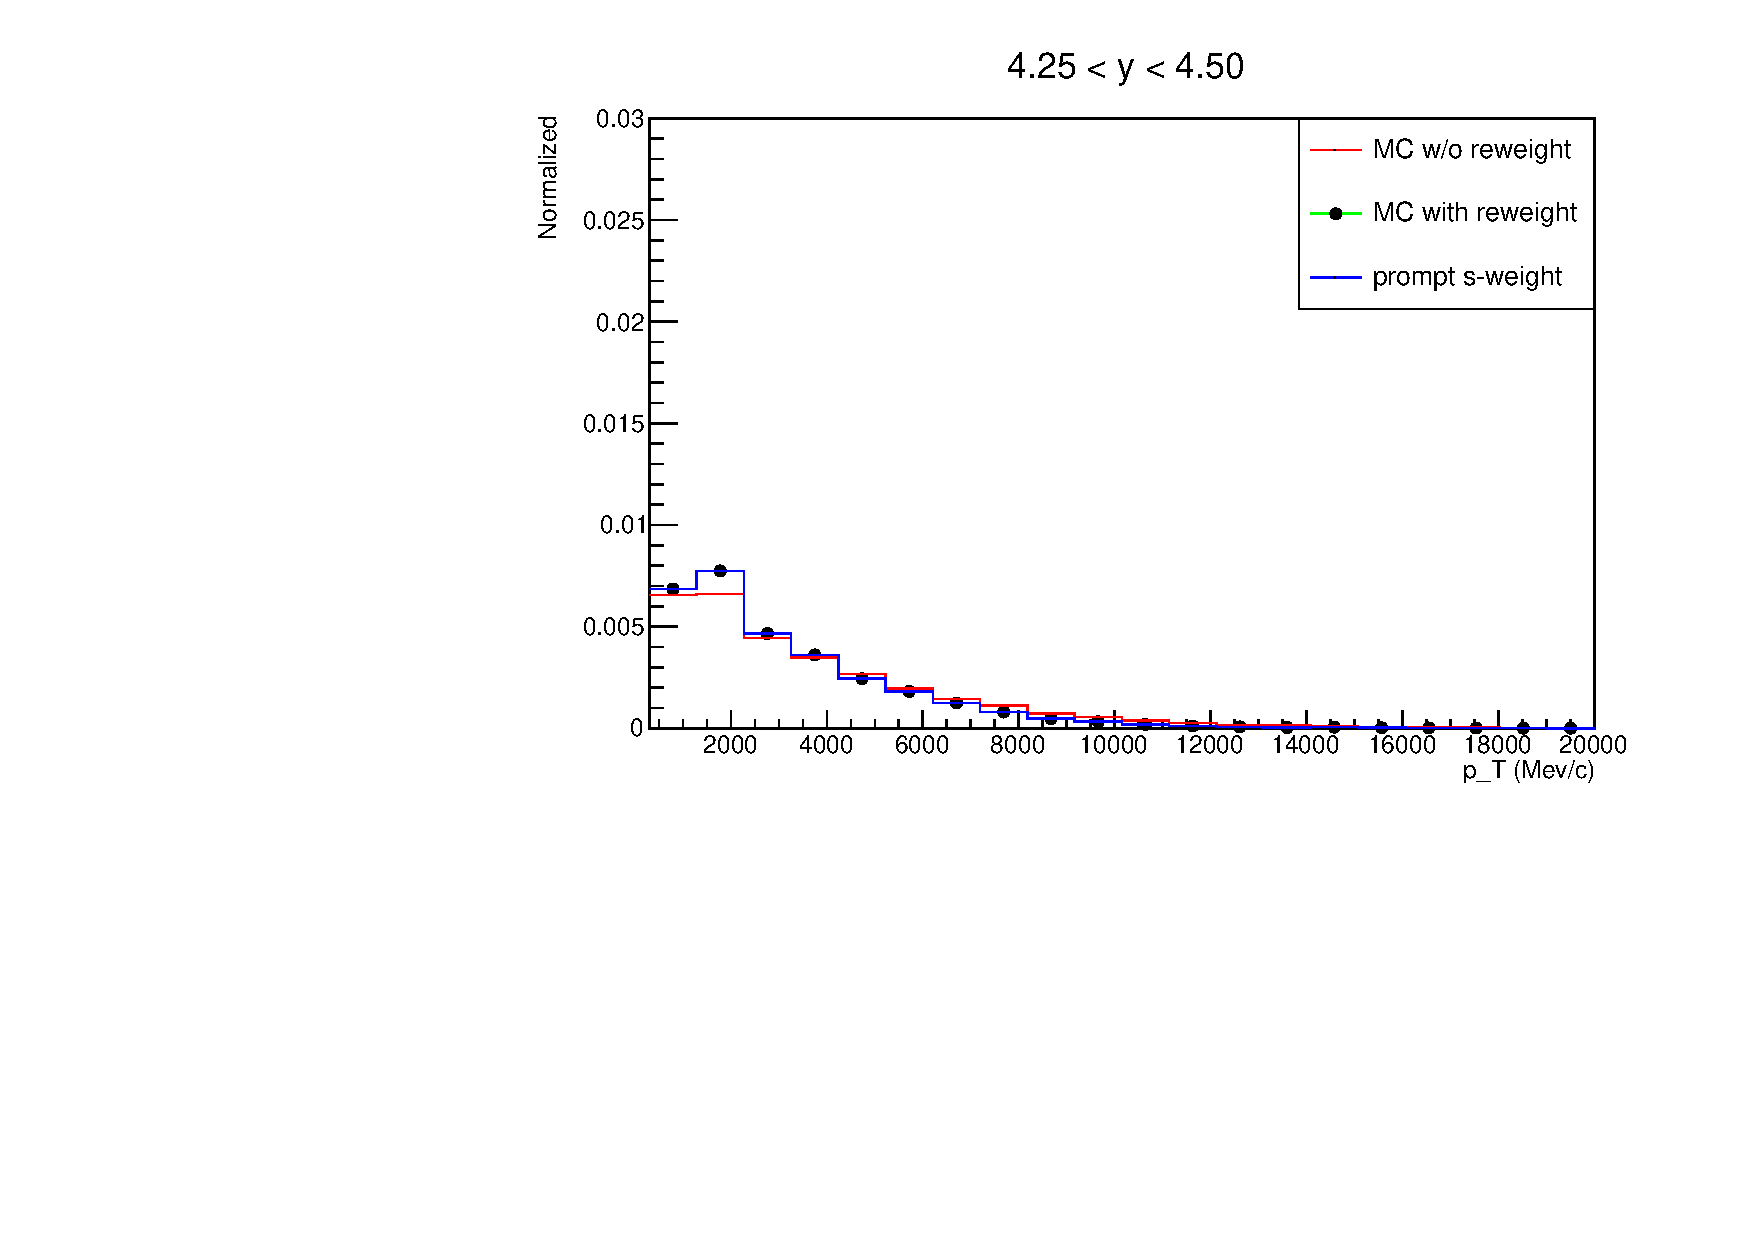
\includegraphics[width=0.19\linewidth]{pdf/Psi2S/reweight/Yp10.pdf}
      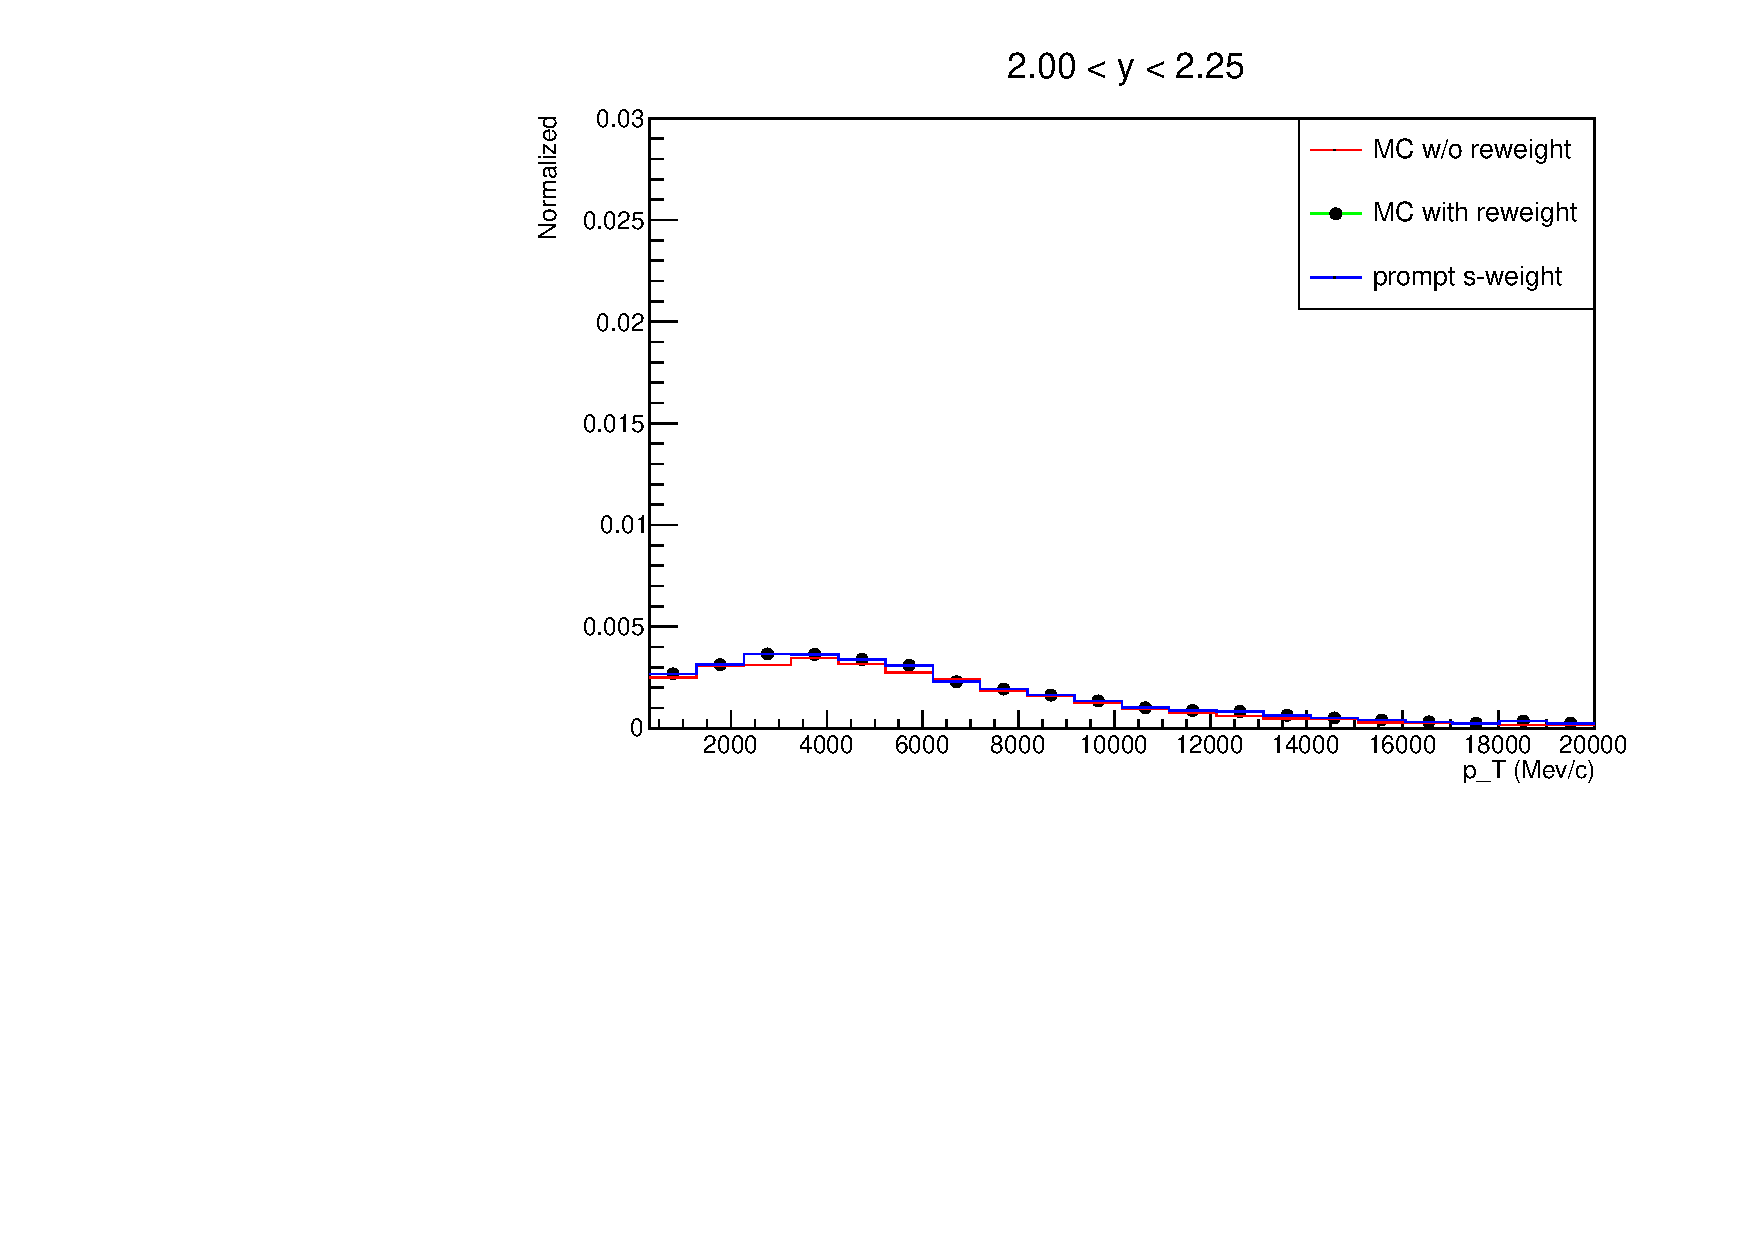
\includegraphics[width=0.19\linewidth]{pdf/Psi2S/reweight/Yb1.pdf}
      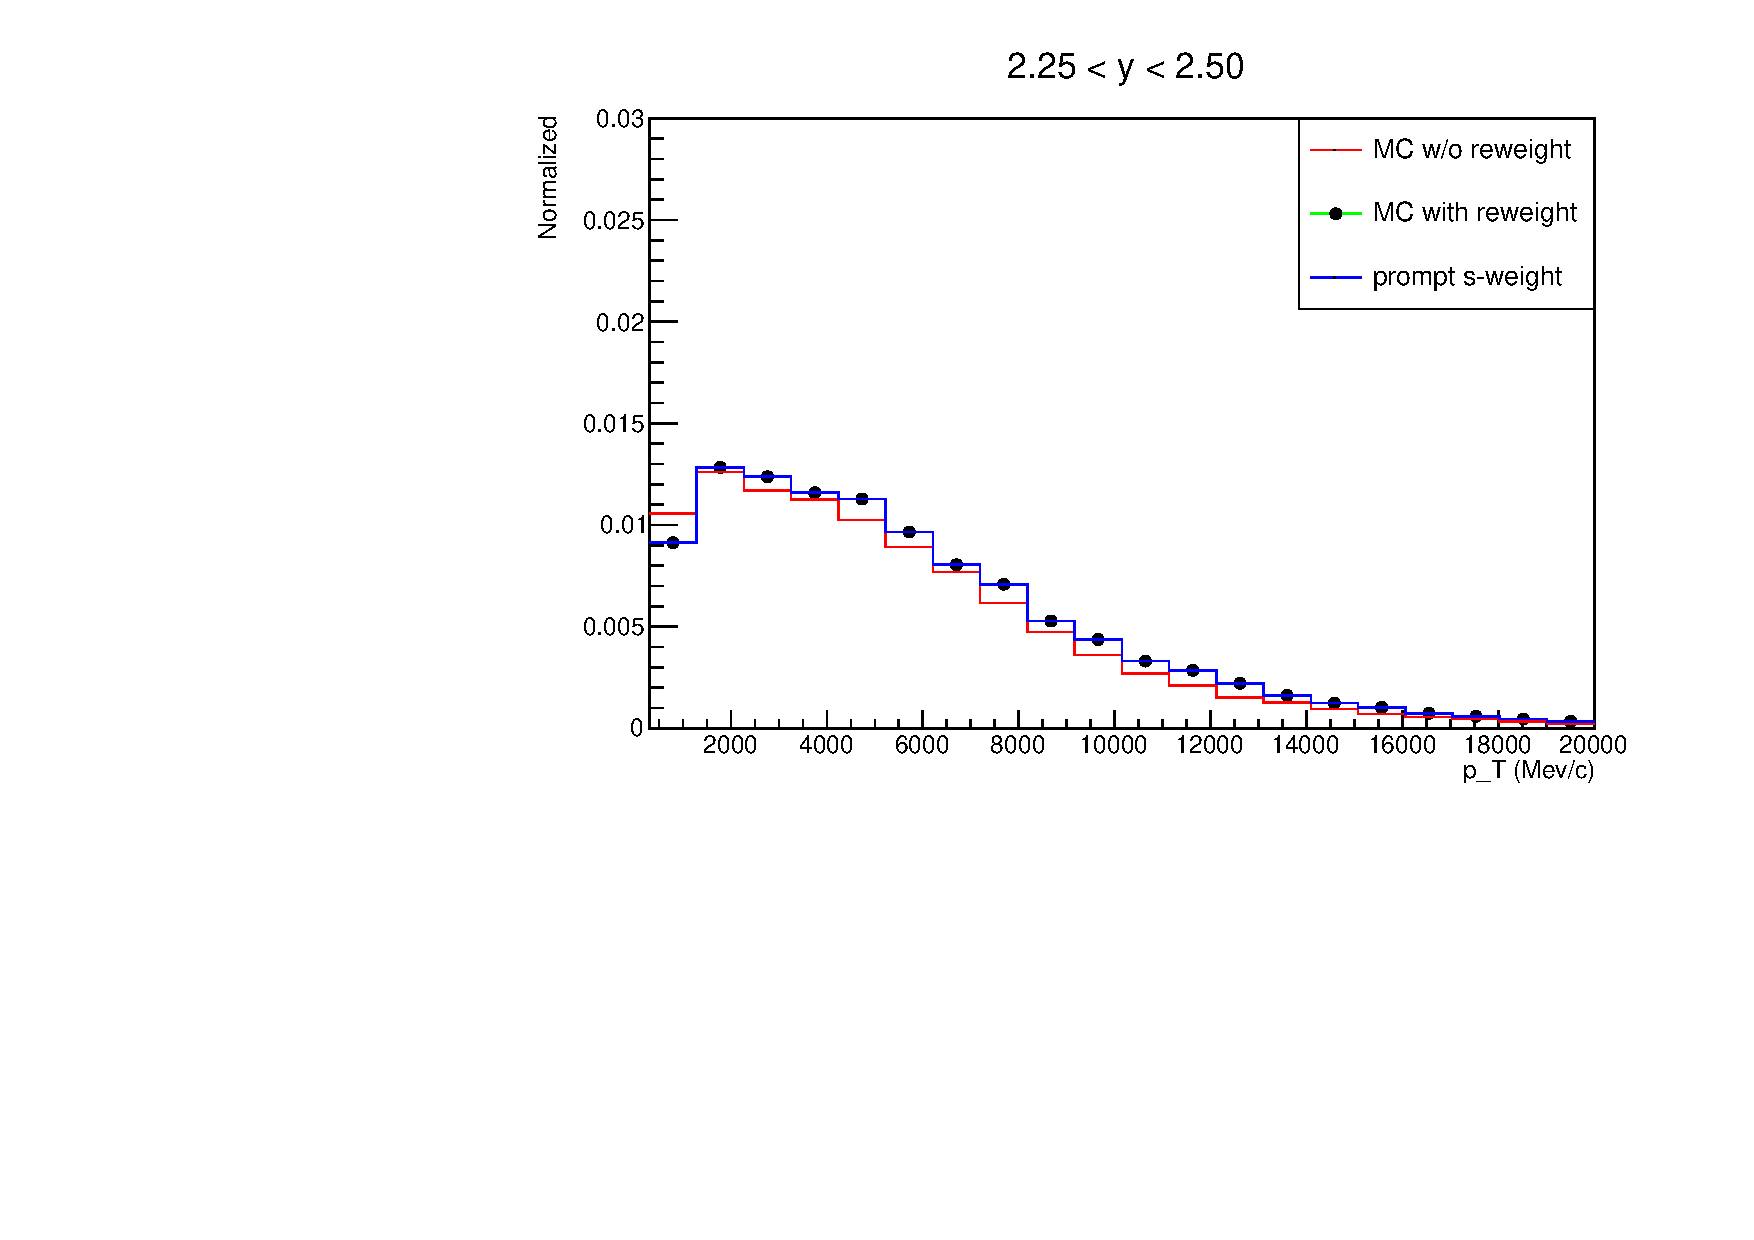
\includegraphics[width=0.19\linewidth]{pdf/Psi2S/reweight/Yb2.pdf} 
      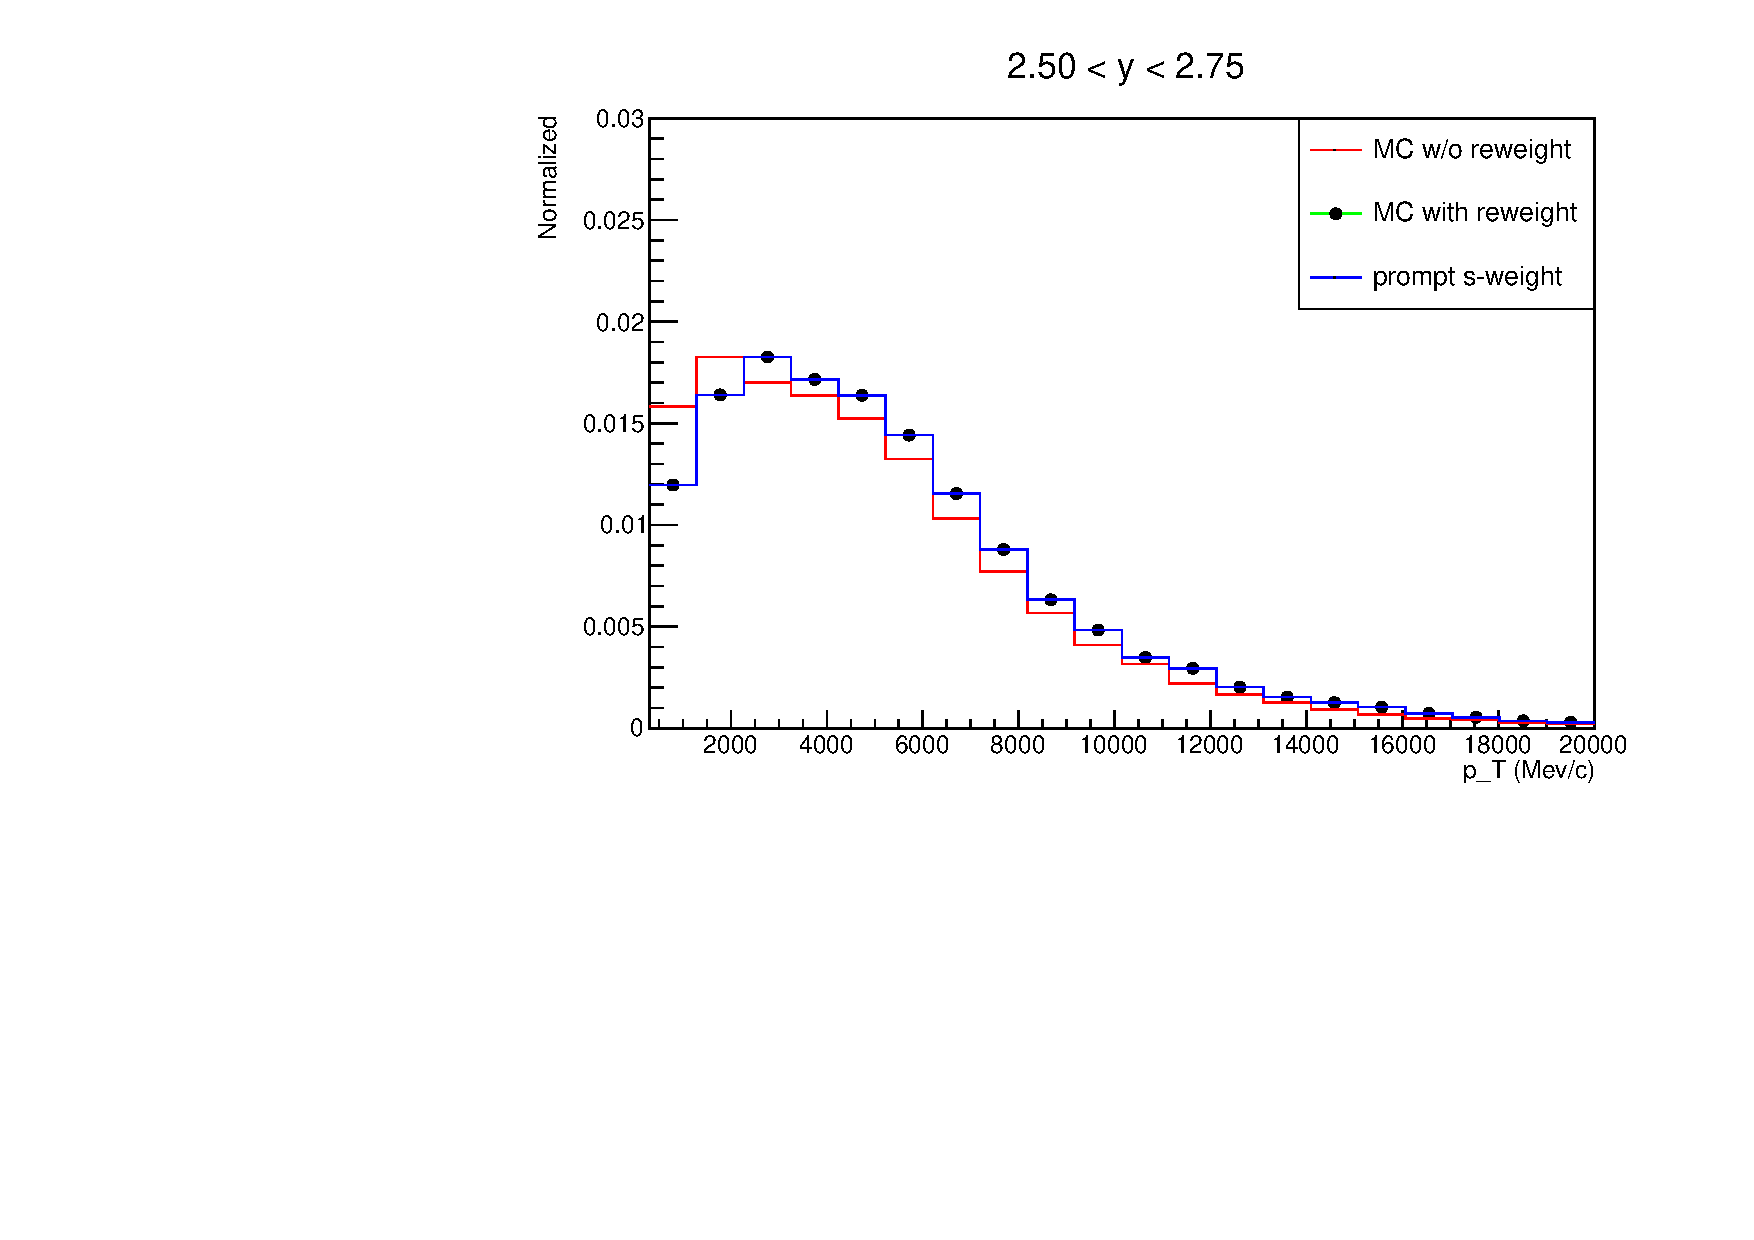
\includegraphics[width=0.19\linewidth]{pdf/Psi2S/reweight/Yb3.pdf}
      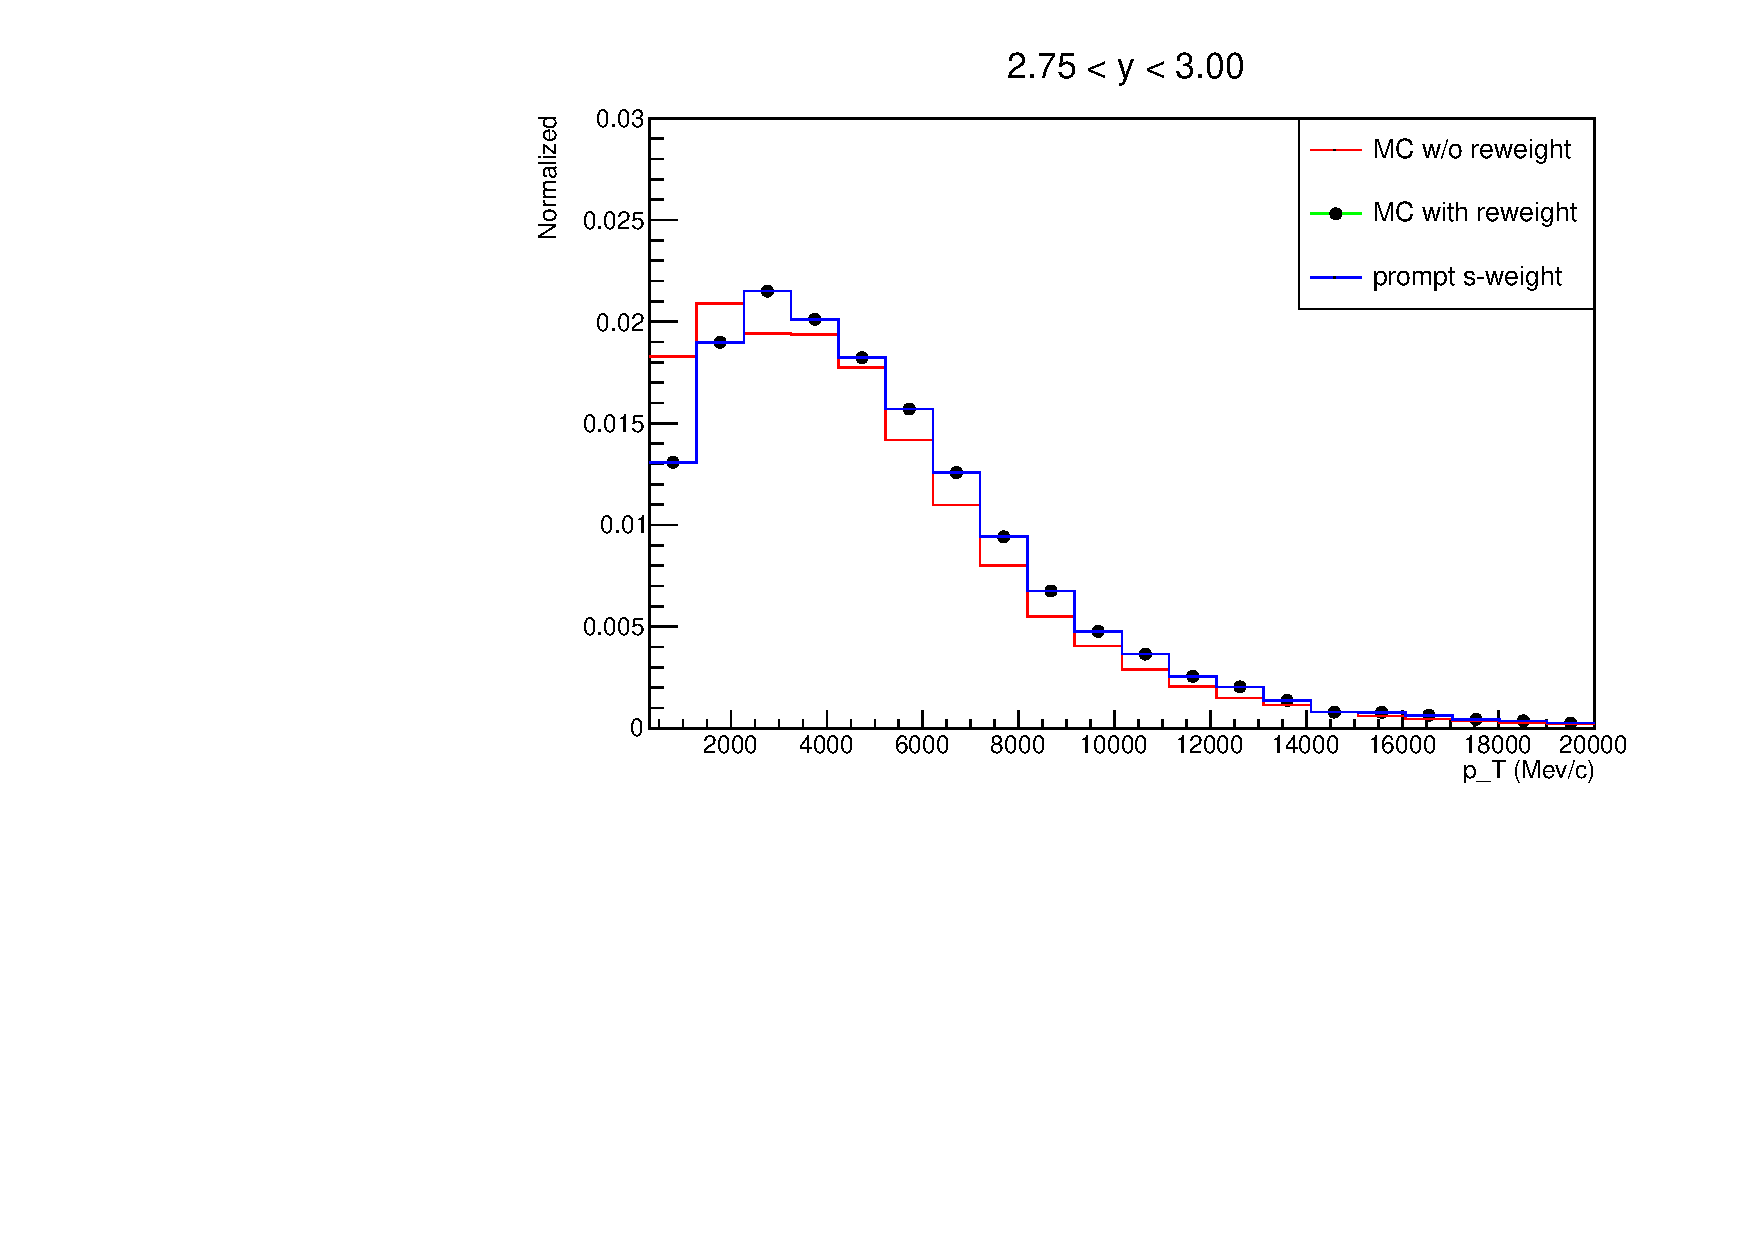
\includegraphics[width=0.19\linewidth]{pdf/Psi2S/reweight/Yb4.pdf}
      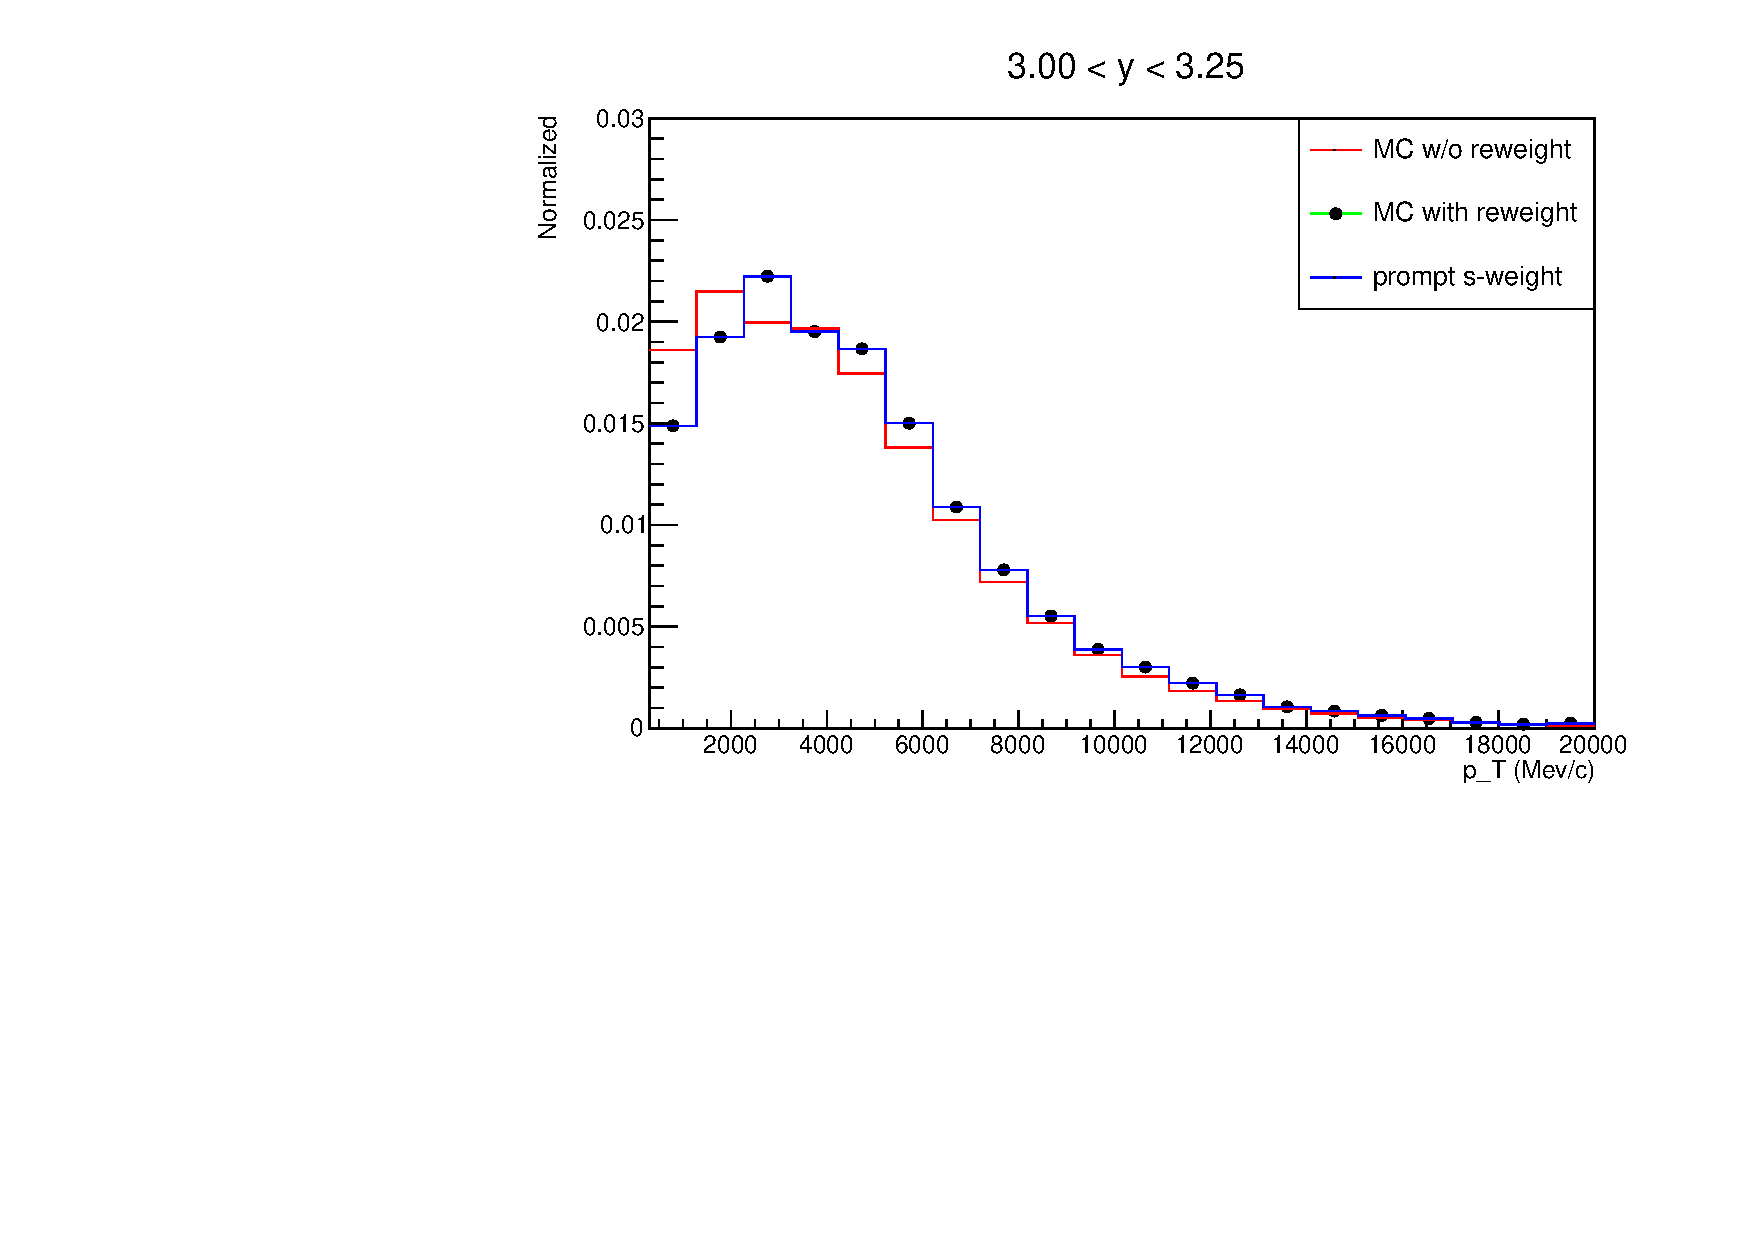
\includegraphics[width=0.19\linewidth]{pdf/Psi2S/reweight/Yb5.pdf}
      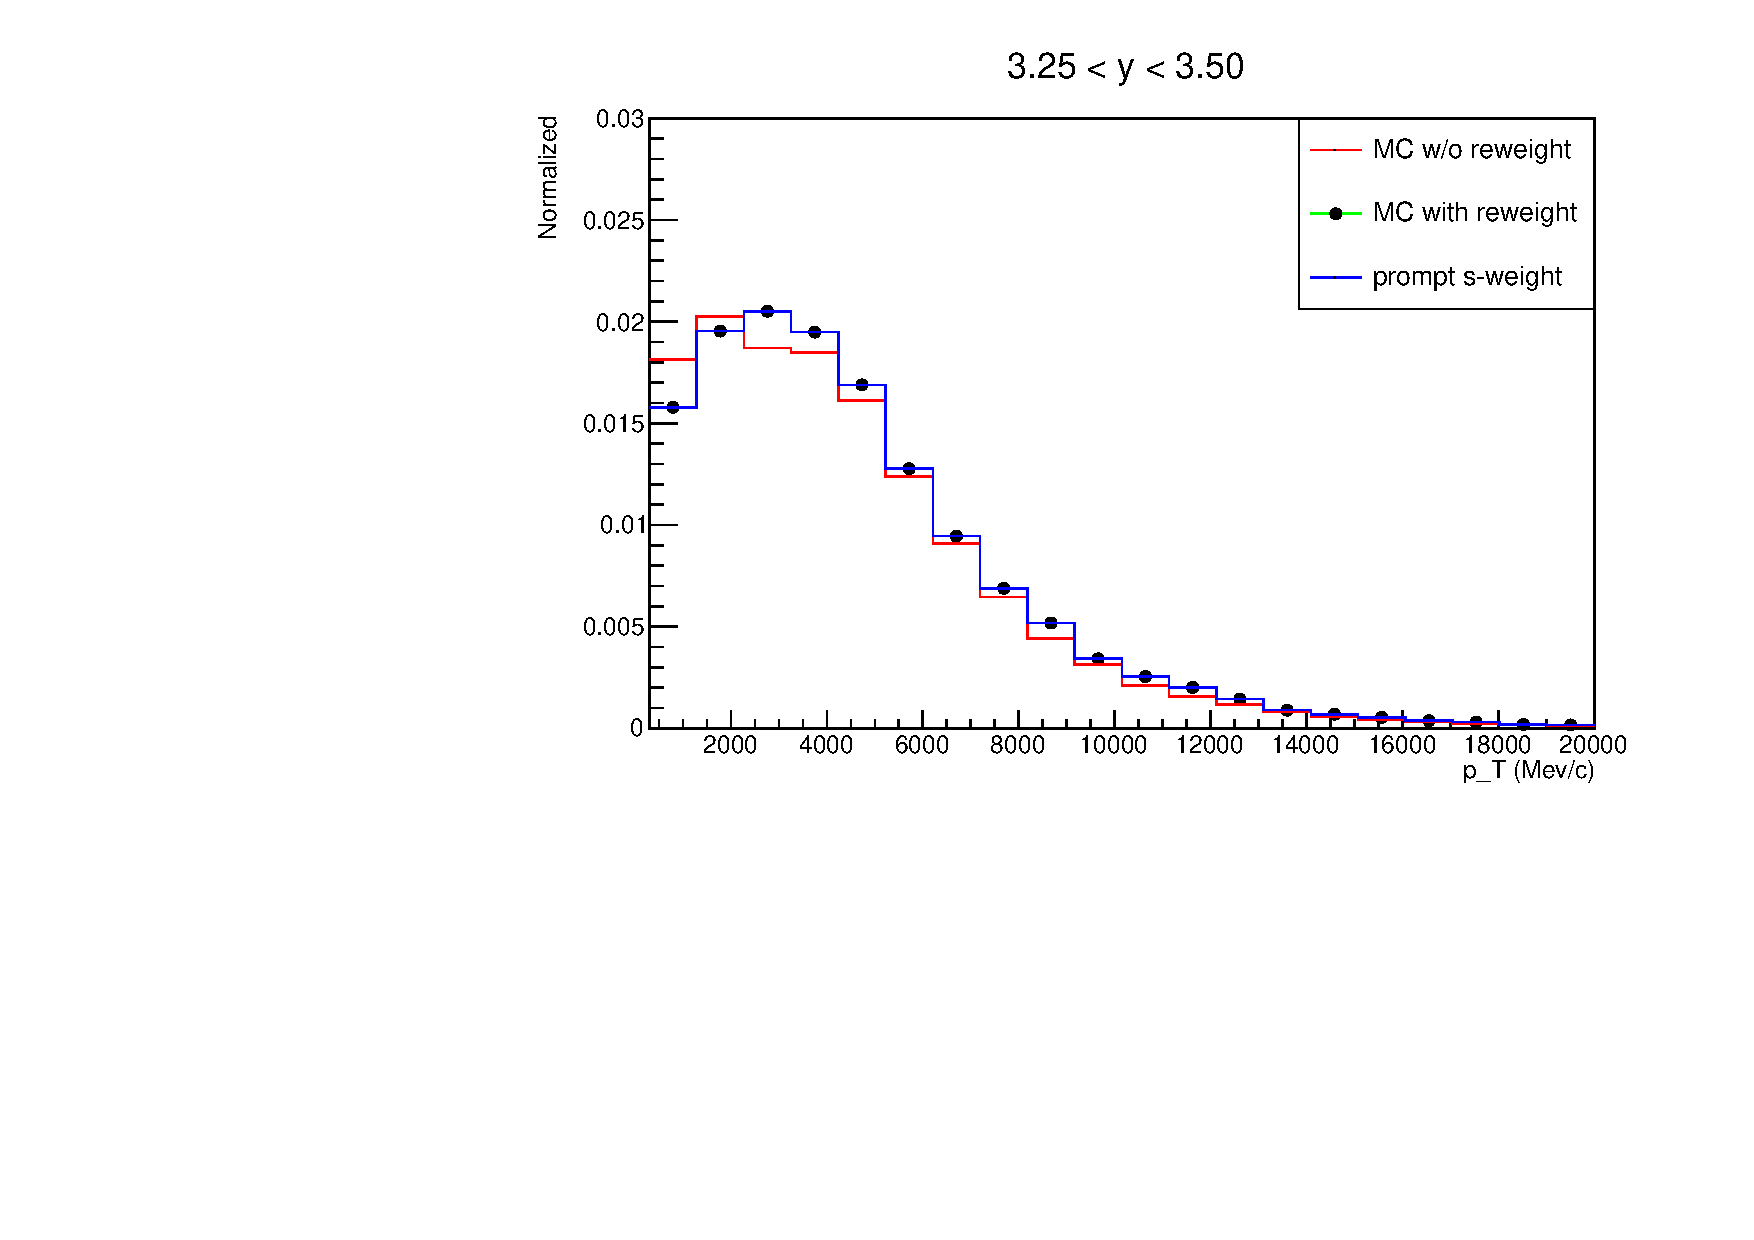
\includegraphics[width=0.19\linewidth]{pdf/Psi2S/reweight/Yb6.pdf}
      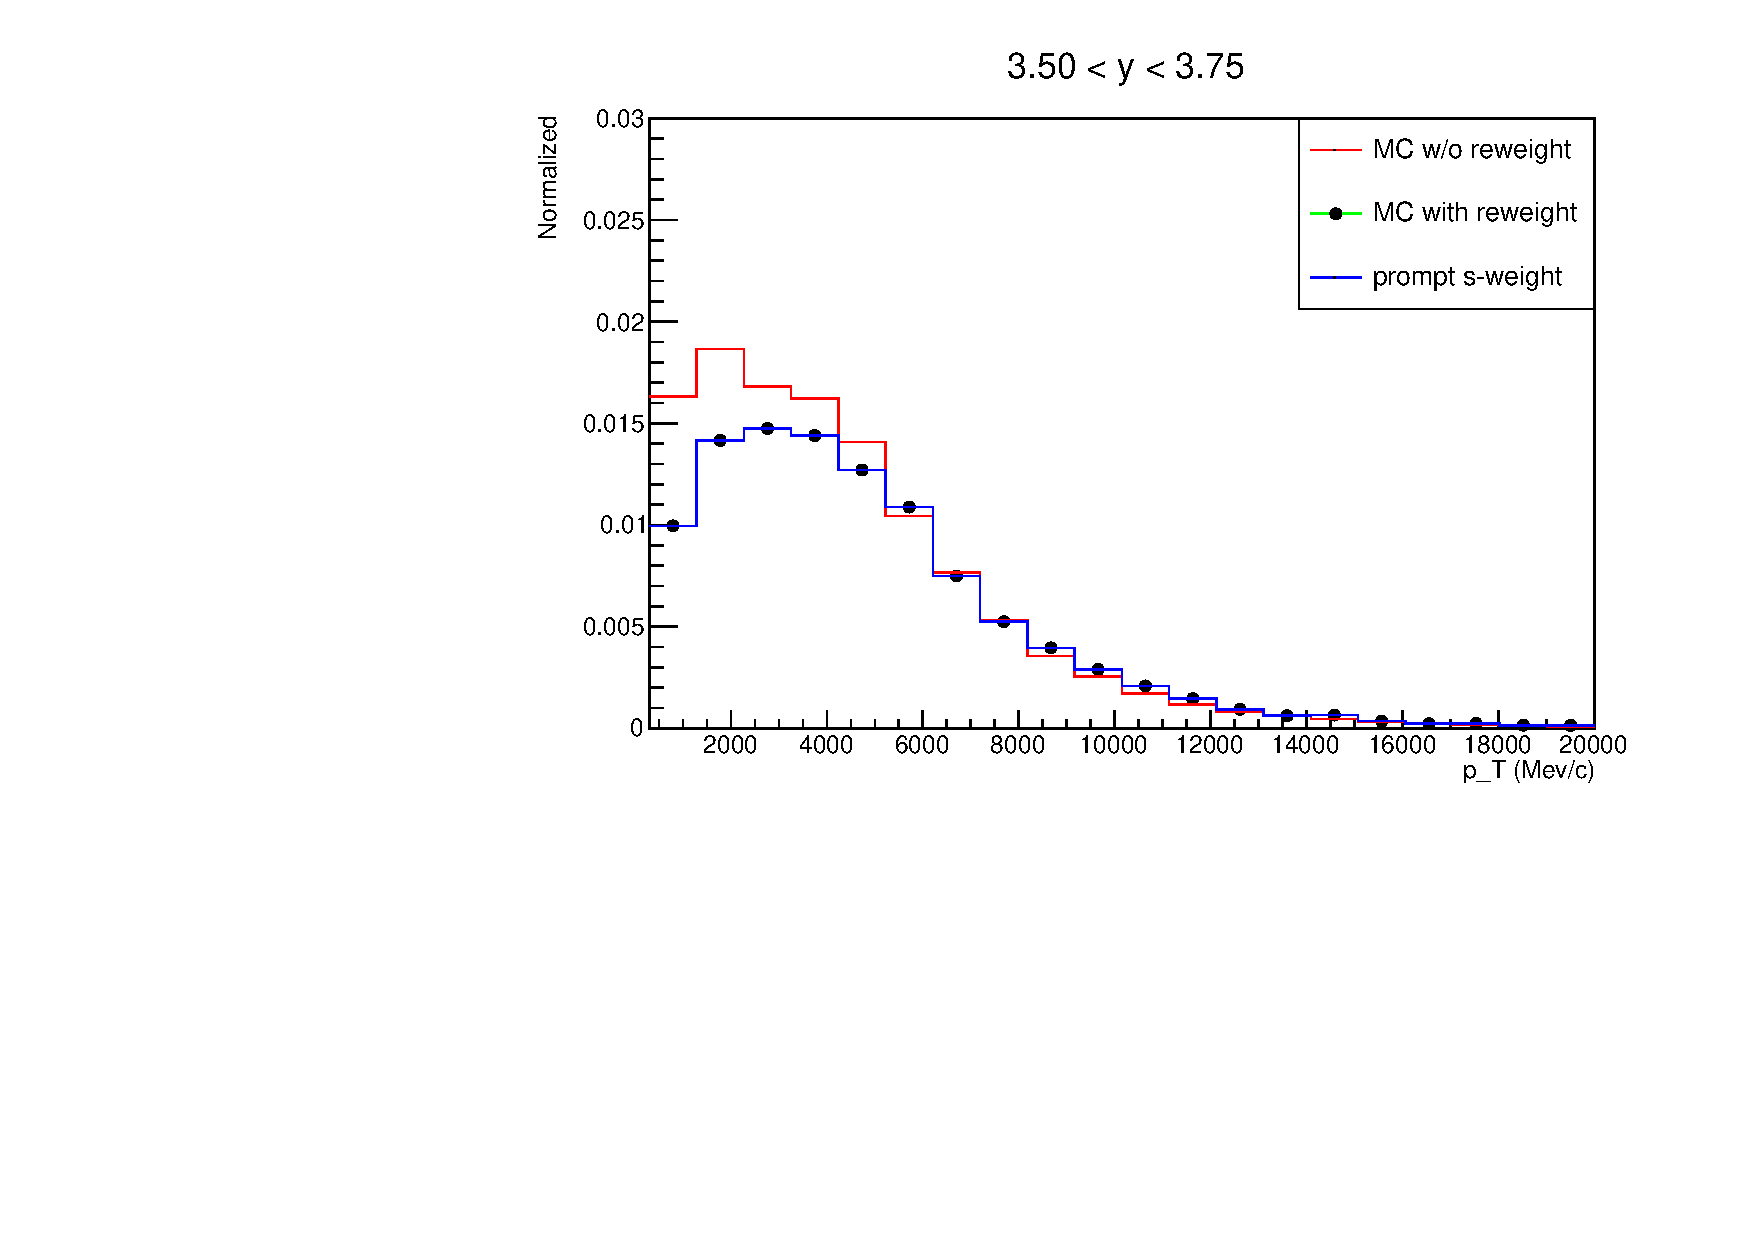
\includegraphics[width=0.19\linewidth]{pdf/Psi2S/reweight/Yb7.pdf}
      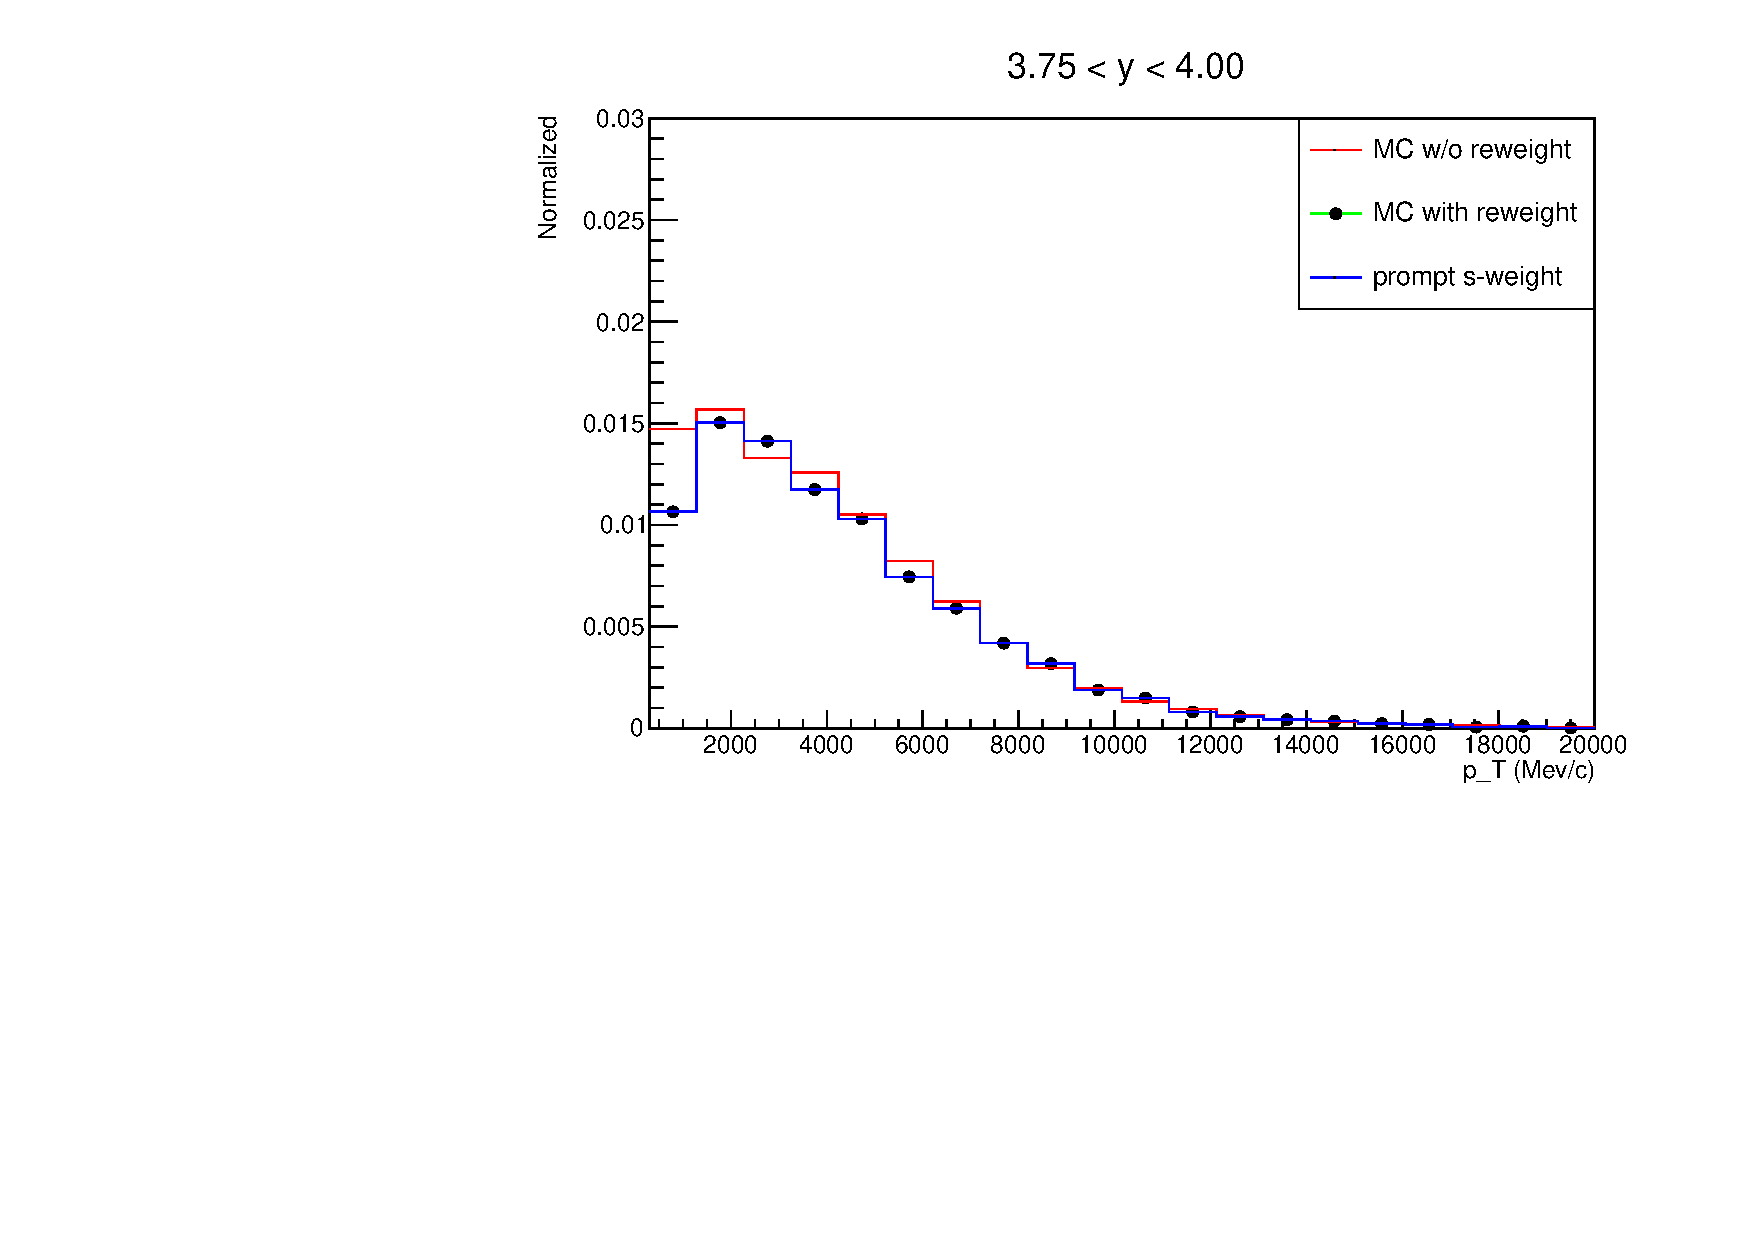
\includegraphics[width=0.19\linewidth]{pdf/Psi2S/reweight/Yb8.pdf}
      \includegraphics[width=0.19\linewidth]{pdf/Psi2S/reweight/Yb9.pdf}
      \includegraphics[width=0.19\linewidth]{pdf/Psi2S/reweight/Yb10.pdf}
    \end{center}
    \caption{
        Reweight the \pt-$y$ distribution to match MC to s-weight data. The first two rows are results of prompt \psitwos and the rest two rows are that of non-prompt \psitwos. } 
    \label{PreweightPTY}
\end{figure}
	
%==============================================================================================================================
\subsection{Geometrical acceptance}
The geometrical acceptance in each kinematic bin is defined as
\begin{equation}
\effAcc \equiv \frac{\mbox{N($\pt$,y) with both $\mu$ in \lhcb acceptance}}{\mbox{N($\pt$,y)}}. 
\end{equation}
The \lhcb acceptance means the polar angle $[10,400]\mrad$ defined with respect to the direction of 
\lhcb $z$-axis, before the effect of the magnetic field. The efficiency $\effAcc$ is determined using 
a simulated sample at the generator level. In Fig.~\ref{EffAcc}, the efficiency in each $\pt$ and 
$y$ bin of \jpsi and \psitwos mesons for $PVZ>-60mm$ and $nPVs=1$ are presented. The geometrical acceptances 
for prompt production and production from $b$-hadron decay are calculated separately for both \jpsi and 
\psitwos. And since the geometrical acceptance is only a function of kinematic variables, we assume that 
there is no difference between the geometrical acceptance between different multiplicity regions.

\begin{figure}[!tbp]
  \begin{center}
    \includegraphics[width=0.49\linewidth]{pdf/Jpsi/eff_acc/eff_prompt_point.pdf}
    \includegraphics[width=0.49\linewidth]{pdf/Psi2S/eff_acc/eff_prompt_point.pdf}
    \vspace*{-0.5cm}
    \includegraphics[width=0.49\linewidth]{pdf/Jpsi/eff_acc/eff_fromb_point.pdf}
    \includegraphics[width=0.49\linewidth]{pdf/Psi2S/eff_acc/eff_fromb_point.pdf}
  \end{center}
  \caption{
    Efficiency of geometrical acceptance for both \jpsi and \psitwos for PVNTRACKS in 4 to 20, where the 
    left is that of \jpsi and the right is of \psitwos. The first row is that of prompt signals and the 
    second row is that of non-prompt signals.}
  \label{EffAcc}
\end{figure}

%==============================================================================================================================
\subsection{Reconstruction-selection efficiency}
The reconstruction and selection efficiency in each kinematic bin is estimated as
\begin{equation}
\effReco  \equiv \frac{\mbox{N($\pt$,y) reconstructed and selected (w/o $\mu$ ID)}}{\mbox{N($\pt$,y) with both $\mu$ in LHCb acceptance}}.
\end{equation}
It includes the efficiency of reconstructing the two muon tracks and the selection of the signals, with the selection criteria listed in Table~\ref{Table32} (excluding muon identification and the trigger). 
Then the reconstruction efficiency is further corrected using the data-over-simulation single tracking efficiency ratio.
The ratio of tracking efficiencies for a single track in data and simulation determined with the Long Tag-Probe method~\cite{LHCb-DP-2013-002} is shown in Fig.~\ref{TrackEfficiencyCalib}, which was given by the tracking group.
\begin{figure}[H]
  \begin{center}
    \includegraphics[width=0.8\linewidth]{pdf/TrackCalib.pdf}
  \end{center}
  \caption{
    Tracking efficiency ratio between data and MC2016 simulation in bins of $p_{\mu}$ and $\eta_{\mu}$ 
    of the muon.}
  \label{TrackEfficiencyCalib}
\end{figure}
For a given event the correction factor is determined by multiplying the efficiency ratios for each of the tracks in the final state. The reweight for prompt and non-prompt signals are done separately with the sWeight extracted from two-dimensional fit. 
For each $\pt$ and $y$ bin, the efficiency of \effReco is shown in Fig.~\ref{EffRec} for PVNTRACKS between 4 to 20. Results in other multiplicity regions are shown in Sec~\ref{sec:EffTables}.
\begin{figure}[!tbp]
  \begin{center}
    \includegraphics[width=0.49\linewidth]{pdf/Jpsi/eff_rec_sel/n1_eff_rec_sel_prompt_point.pdf}
    \includegraphics[width=0.49\linewidth]{pdf/Psi2S/eff_rec_sel/n1_eff_rec_sel_prompt_point.pdf}
    \vspace*{-0.5cm}
    \includegraphics[width=0.49\linewidth]{pdf/Jpsi/eff_rec_sel/n1_eff_rec_sel_fromb_point.pdf}
    \includegraphics[width=0.49\linewidth]{pdf/Psi2S/eff_rec_sel/n1_eff_rec_sel_fromb_point.pdf}
  \end{center}
  \caption{
    Efficiency of reconstruction and selection (excluding muon identification and the trigger) for both \jpsi and \psitwos for PVNTRACKS in 4 to 20, where the 
    left is that of \jpsi and the right is of \psitwos. The first row is that of prompt signals and the 
    second row is that of non-prompt signals.}
  \label{EffRec}
\end{figure}
%==============================================================================================================================
\subsection{Muon identification efficiency}
The muon identification requirement used in this analysis is ${\rm IsMuon}==1\&\& {\rm DLLmu}>2 \&\& {\rm ProbNNmu}>0.8$. 
The efficiency is introduced by 
\begin{equation}
\effID    \equiv \frac{\mbox{N($\pt$,y) selected including $\mu$ID requirement}}{\mbox{N($\pt$,y) reconstructed and selected (w/o $\mu$ID)}}.
\end{equation}

The Muon ID efficiency is obtained using simulated samples and calibrated with the data using the PIDCalib package.
The full simulated samples used here are selected by all the selections except the muon ID and the trigger.
The selected samples are the same as the ones used in the reconstruction and selection.
As estimating the reconstruction and selection efficiency, we first reweight the multiplicity variable according to the variable we used to divide the multiplicity, and \pt-$y$ spectrum.
The muon ID efficiency in each (\pt,$y$) bin is then calculated by averaging the muon ID efficiency of each candidate in the bin, which is the product of the muon ID efficiencies of the two muons from the efficiency table, obtained from the PIDCalib package, according to their $(p,\eta,{\rm nSPDhits})$ values. 
The formula is
\begin{equation}
\overline{\epsilon}(\pt,y)=\frac{\sum \epsilon_\mup(p_\mup,\eta_\mup,\mathrm{nSPDhits})\epsilon_\mun(p_\mun,\eta_\mun,\mathrm{nSPDhits})}{N_\mathrm{res\&sel}}.
\label{eq:muonid}
\end{equation}
where $\epsilon_\mup(p_\mup,\eta_\mup,\mathrm{nSPDhits})$ and $\epsilon_\mun(p_\mun,\eta_\mun,\mathrm{nSPDhits})$ are the muon ID efficiencies obtained from the efficiency table.
The efficiency table we used here is from the calibration sample which contains \jpsi candidates taken in the same period and the average efficiency over the whole period is used.
One 3-Dimensional efficiency table dedicated to the muon ID selection is obtained from this calibration sample in bins of the muon $\mathrm{(p,\eta,\mathrm{nSPDhits})}$ using the tag-and-probe method.
The MagDown and MagUp efficiencies are calculated separately.
For the muon candidates whose $(p, \eta,\mathrm{nSPDhits})$ are out of the range of the calibration sample, we simply set the value to be one due to the fact that the production in those bins is significantly small.
For each $\pt$ and $y$ bin, the efficiency of \effID is shown in Fig.~\ref{EffID}. Results in other multiplicity regions are shown in Sec~\ref{sec:EffTables}.
\begin{figure}[!tbp]
  \begin{center}
    \includegraphics[width=0.49\linewidth]{pdf/Jpsi/eff_pid/n1_eff_pid_prompt_point.pdf}
    \includegraphics[width=0.49\linewidth]{pdf/Psi2S/eff_pid/n1_eff_pid_prompt_point.pdf}
    \vspace*{-0.5cm}
    \includegraphics[width=0.49\linewidth]{pdf/Jpsi/eff_pid/n1_eff_pid_fromb_point.pdf}
    \includegraphics[width=0.49\linewidth]{pdf/Psi2S/eff_pid/n1_eff_pid_fromb_point.pdf}
  \end{center}
  \caption{
    PID efficiencies for both \jpsi and \psitwos for PVNTRACKS in 4 to 20, where the 
    left is that of \jpsi and the right is of \psitwos. The first row is that of prompt signals and the 
    second row is that of non-prompt signals.}
  \label{EffID}
\end{figure}
%==============================================================================================================================
\subsection{Trigger efficiency}
The trigger efficiency in each kinematic bin is defined as 
\begin{equation}
\effTrigger \equiv \frac{\mbox{N($\pt$,y) triggered}}{\mbox{N($\pt$,y) selected including $\mu$ID requirement}} 
\end{equation}
Here the triggers include both TOS requirements of \texttt{L0DiMuon}, \texttt{Hlt1DiMuonHighMass} for both, and \texttt{Hlt2DiMuonJPsiTurbo} for \jpsi and \texttt{Hlt2DiMuonPsi2STurbo} for \psitwos, respectively. 
Only \texttt{L0DiMuon} and \texttt{Hlt1DiMuonHighMass} contribute actually to the efficiency because the \texttt{Hlt2DiMuonJPsiTurbo} and \texttt{Hlt2DiMuonPsi2STurbo} is almost fully efficient due to the facts that the offline selections are tighter.
For each $\pt$ and $y$ bin, the efficiencies of \effTrigger for both \jpsi and \psitwos from different sources for PVNTRACKS between 4 to 20 are shown in Fig.~\ref{EffTrigger}. Results in other multiplicity regions are shown in Sec~\ref{sec:EffTables}.
\begin{figure}[!tbp]
  \begin{center}
    \includegraphics[width=0.49\linewidth]{pdf/Jpsi/eff_trigger/n1_eff_trigger_prompt_point.pdf}
    \includegraphics[width=0.49\linewidth]{pdf/Psi2S/eff_trigger/n1_eff_trigger_prompt_point.pdf}
    \vspace*{-0.5cm}
    \includegraphics[width=0.49\linewidth]{pdf/Jpsi/eff_trigger/n1_eff_trigger_fromb_point.pdf}
    \includegraphics[width=0.49\linewidth]{pdf/Psi2S/eff_trigger/n1_eff_trigger_fromb_point.pdf}
  \end{center}
  \caption{
    Trigger efficiencies for both \jpsi and \psitwos for PVNTRACKS in 4 to 20, where the 
    left is that of \jpsi and the right is of \psitwos. The first row is that of prompt signals and the 
    second row is that of non-prompt signals.}
  \label{EffTrigger}
\end{figure}
%==============================================================================================================================
\subsection{Total efficiency}
The total efficiencies \effTot for \jpsi and \psitwos from different sources for PVNTRACKS between 4 to 20 are shown in Fig.~\ref{EffTot}. Results in other multiplicity regions are shown in Sec~\ref{sec:EffTables}.
The separate efficiencies for prompt and non-prompt signals are used to calculate the final cross-section.
\begin{figure}[!tbp]
  \begin{center}
    \includegraphics[width=0.49\linewidth]{pdf/Jpsi/eff_tot/n1_prompt_point.pdf}
    \includegraphics[width=0.49\linewidth]{pdf/Psi2S/eff_tot/n1_prompt_point.pdf}
    \vspace*{-0.5cm}
    \includegraphics[width=0.49\linewidth]{pdf/Jpsi/eff_tot/n1_fromb_point.pdf}
    \includegraphics[width=0.49\linewidth]{pdf/Psi2S/eff_tot/n1_fromb_point.pdf}
  \end{center}
  \caption{
    Total efficiencies for both \jpsi and \psitwos for PVNTRACKS in 4 to 20, where the 
    left is that of \jpsi and the right is of \psitwos. The first row is that of prompt signals and the 
    second row is that of non-prompt signals.}
  \label{EffTot}
\end{figure}

\subsection{Variation due to different reweight samples}
Since the multiplicity-dependent breakup effects may vary with (\pt, $y$), the two-dimensional (\pt, $y$) distribution may differ in different multiplicity region. To study this effect, the (\pt, $y$) spectra are prepared for three different multiplicity classes:
\begin{itemize}
	\item Data sample with all selections of PVNTRACKS.
	\item Data sample with PVNTRACKS$>=60$ as high-multiplicity sample, where 60 is the bin edge of the second to last bin of \pt binning scheme.
	\item Data sample with PVNTRACKS$<60$ as low-multiplicity sample.
\end{itemize}	
 The (\pt,$y$) distributions of high- and low-multiplicity samples are shown in Figs.~\ref{HighLowDist}. 
With this two samples for (\pt, $y$) reweight, we can calculate the ratio of total efficiencies for both prompt and non-prompt \jpsi and \psitwos in each multiplicity region. And after comparing the newly calculated ratio of total efficiencies with the original one, we record the variation in each (\pt, $y$, PVNTRACKS) bin in form of a certain time of statistical uncertainty in that bin. And the result is shown in Figs~\ref{HighLow}. It's clearly shown that all the variations are within uncertainties, where the center values and uncertainties for ratio of efficiencies are from the results reweighted by the full-multiplicity sample.
\begin{figure}[h]
  \begin{center}
    \includegraphics[width=0.49\linewidth]{pdf/Jpsi/reweight/promptHighLowPTY.pdf}
    \includegraphics[width=0.49\linewidth]{pdf/Psi2S/reweight/promptHighLowPTY.pdf}
    \vspace*{-0.5cm}
    \includegraphics[width=0.49\linewidth]{pdf/Jpsi/reweight/frombHighLowPTY.pdf}
    \includegraphics[width=0.49\linewidth]{pdf/Psi2S/reweight/frombHighLowPTY.pdf}
  \end{center}
  \caption{
    Two-dimensional (\pt, $y$) distribution for prompt and non-prompt \jpsi and \psitwos of different samples (high-multiplicity sample in red).}
  \label{HighLowDist}
\end{figure}

\begin{figure}[h]
  \begin{center}
	  \includegraphics[width=0.6\linewidth]{pdf/HighLow.pdf}
  \end{center}
\caption{
	Distribution of the variation due to different reweight samples recorded in times of the statistical uncertainty.}
\label{HighLow}
\end{figure}

